\documentclass[a4paper]{report}

% basics
\usepackage[utf8]{inputenc}
\usepackage[T1]{fontenc}
\usepackage{textcomp}
% \usepackage[dutch]{babel}
\usepackage{url}
\usepackage{hyperref}
\hypersetup{
    colorlinks,
    linkcolor={black},
    citecolor={black},
    urlcolor={blue!80!black},
    % backref=true, 
    % pagebackref=true
}
% Page Margins
\usepackage[
    margin=2.5cm, 
    % top=2.8cm, bottom=2.8cm,
    % left=1in, right=1in, 
    % headheight=14.5pt
    ]{geometry}

\usepackage{setspace}
\setstretch{1.15}

\usepackage{graphicx}
\usepackage{float}
\usepackage{booktabs}
\usepackage{pdfpages}
\usepackage[shortlabels]{enumitem}
% \usepackage{parskip}
\usepackage{emptypage}
\usepackage{subcaption}
\usepackage{multicol}
\usepackage[usenames,dvipsnames]{xcolor}

% \usepackage{cmbright}

\usepackage{amsmath, amsfonts, mathtools, amsthm, amssymb}
\usepackage{mathrsfs}
% \usepackage{dutchcal} % \mathcal: also small letters. \mathbcal = bold ones. % https://tex.stackexchange.com/a/641540/114006
\usepackage{braket} % https://tex.stackexchange.com/a/253232/114006
\usepackage{cancel}
\usepackage{bm}
\usepackage[ruled,vlined,linesnumbered]{algorithm2e} % SeniorMars template
% \usepackage{lipsum}
\usepackage{pgfplots}
\usepgfplotslibrary{fillbetween}

\newcommand\N{\ensuremath{\mathbb{N}}}
\newcommand\R{\ensuremath{\mathbb{R}}}
\newcommand\Z{\ensuremath{\mathbb{Z}}}
\renewcommand\O{\ensuremath{\emptyset}}
\newcommand\Q{\ensuremath{\mathbb{Q}}}
\newcommand\C{\ensuremath{\mathbb{C}}}
\DeclareMathOperator{\sgn}{sgn}
\usepackage{systeme}
\let\svlim\lim\def\lim{\svlim\limits}
\let\implies\Rightarrow
\let\impliedby\Leftarrow
\let\iff\Leftrightarrow
\let\epsilon\varepsilon
\usepackage{stmaryrd} % for \lightning
\newcommand\contra{\scalebox{1.1}{$\lightning$}}
% \let\phi\varphi





% correct
\definecolor{correct}{HTML}{009900}
\newcommand\correct[2]{\ensuremath{\:}{\color{red}{#1}}\ensuremath{\to }{\color{correct}{#2}}\ensuremath{\:}}
\newcommand\green[1]{{\color{correct}{#1}}}



% horizontal rule
\newcommand\hr{
    \noindent\rule[0.5ex]{\linewidth}{0.5pt}
}


% hide parts
\newcommand\hide[1]{}



% si unitx
\usepackage{siunitx}
\sisetup{locale = FR}
% \renewcommand\vec[1]{\mathbf{#1}}
\newcommand\mat[1]{\mathbf{#1}}


% tikz
\usepackage{tikz}
\usepackage{tikz-cd}
\usepackage{tikzsymbols} % for symbols such as smiley
\usetikzlibrary{intersections, angles, quotes, calc, positioning}
\usetikzlibrary{arrows.meta}
\usepackage{pgfplots}
\pgfplotsset{compat=1.13}


\tikzset{
    force/.style={thick, {Circle[length=2pt]}-stealth, shorten <=-1pt}
}


% theorems
\usepackage{thmtools}
\usepackage[framemethod=TikZ]{mdframed}
% \mdfsetup{skipabove=1em,skipbelow=0em, innertopmargin=5pt, innerbottommargin=6pt}


\theoremstyle{definition}

\makeatletter


\@ifclasswith{report}{nocolor}{
    \declaretheoremstyle[headfont=\bfseries\sffamily, bodyfont=\normalfont, mdframed={ nobreak } ]{thmgreenbox}
    \declaretheoremstyle[headfont=\bfseries\sffamily, bodyfont=\normalfont, mdframed={ nobreak } ]{thmredbox}
    \declaretheoremstyle[headfont=\bfseries\sffamily, bodyfont=\normalfont]{thmbluebox}
    \declaretheoremstyle[headfont=\bfseries\sffamily, bodyfont=\normalfont]{thmblueline}
    \declaretheoremstyle[headfont=\bfseries\sffamily, bodyfont=\normalfont, numbered=no, mdframed={ rightline=false, topline=false, bottomline=false, }, qed=\qedsymbol ]{thmproofbox}
    \declaretheoremstyle[headfont=\bfseries\sffamily, bodyfont=\normalfont, numbered=no, mdframed={ nobreak, rightline=false, topline=false, bottomline=false } ]{thmexplanationbox}
    \AtEndEnvironment{eg}{\null\hfill$\diamond$}%
}{
    \declaretheoremstyle[
      headfont=\bfseries\sffamily\color{ForestGreen!70!black}, bodyfont=\normalfont,
      mdframed={
          linewidth=2pt,
          rightline=false, topline=false, bottomline=false,
          linecolor=ForestGreen, backgroundcolor=ForestGreen!5,
          nobreak=false
        }
    ]{thmgreenbox}
    
    \declaretheoremstyle[
      headfont=\bfseries\sffamily\color{ForestGreen!70!black}, bodyfont=\normalfont,
      mdframed={
          linewidth=2pt,
          rightline=false, topline=false, bottomline=false,
          linecolor=ForestGreen, backgroundcolor=ForestGreen!8,
          nobreak=false
        }
    ]{thmgreen2box}
    
    \declaretheoremstyle[
      headfont=\bfseries\sffamily\color{NavyBlue!70!black}, bodyfont=\normalfont,
      mdframed={
          linewidth=2pt,
          rightline=false, topline=false, bottomline=false,
          linecolor=NavyBlue, backgroundcolor=NavyBlue!5,
          nobreak=false
        }
    ]{thmbluebox}
    
    \declaretheoremstyle[
      headfont=\bfseries\sffamily\color{TealBlue!70!black}, bodyfont=\normalfont,
      mdframed={
          linewidth=2pt,
          rightline=false, topline=false, bottomline=false,
          linecolor=TealBlue,
          nobreak=false
        }
    ]{thmblueline}
    
    \declaretheoremstyle[
      headfont=\bfseries\sffamily\color{RawSienna!70!black}, bodyfont=\normalfont,
      mdframed={
          linewidth=2pt,
          rightline=false, topline=false, bottomline=false,
          linecolor=RawSienna, backgroundcolor=RawSienna!5,
          nobreak=false
        }
    ]{thmredbox}
    
    \declaretheoremstyle[
      headfont=\bfseries\sffamily\color{RawSienna!70!black}, bodyfont=\normalfont,
      mdframed={
          linewidth=2pt,
          rightline=false, topline=false, bottomline=false,
          linecolor=RawSienna, backgroundcolor=RawSienna!8,
          nobreak=false
        }
    ]{thmred2box}
    
    \declaretheoremstyle[
      headfont=\bfseries\sffamily\color{SeaGreen!70!black}, bodyfont=\normalfont,
      mdframed={
          linewidth=2pt,
          rightline=false, topline=false, bottomline=false,
          linecolor=SeaGreen, backgroundcolor=SeaGreen!2,
          nobreak=false
        }
    ]{thmgreen3box}
    
    \declaretheoremstyle[
      headfont=\bfseries\sffamily\color{WildStrawberry!70!black}, bodyfont=\normalfont,
      mdframed={
          linewidth=2pt,
          rightline=false, topline=false, bottomline=false,
          linecolor=WildStrawberry, backgroundcolor=WildStrawberry!5,
          nobreak=false
        }
    ]{thmpinkbox}
    
    \declaretheoremstyle[
      headfont=\bfseries\sffamily\color{MidnightBlue!70!black}, bodyfont=\normalfont,
      mdframed={
          linewidth=2pt,
          rightline=false, topline=false, bottomline=false,
          linecolor=MidnightBlue, backgroundcolor=MidnightBlue!5,
          nobreak=false
        }
    ]{thmblue2box}
    
    \declaretheoremstyle[
      headfont=\bfseries\sffamily\color{Gray!70!black}, bodyfont=\normalfont,
      mdframed={
          linewidth=2pt,
          rightline=false, topline=false, bottomline=false,
          linecolor=Gray, backgroundcolor=Gray!5,
          nobreak=false
        }
    ]{notgraybox}
    
    \declaretheoremstyle[
      headfont=\bfseries\sffamily\color{Gray!70!black}, bodyfont=\normalfont,
      mdframed={
          linewidth=2pt,
          rightline=false, topline=false, bottomline=false,
          linecolor=Gray,
          nobreak=false
        }
    ]{notgrayline}
    
    \declaretheoremstyle[
      headfont=\bfseries\sffamily\color{RawSienna!70!black}, bodyfont=\normalfont,
      numbered=no,
      mdframed={
          linewidth=2pt,
          rightline=false, topline=false, bottomline=false,
          linecolor=RawSienna, backgroundcolor=RawSienna!1,
        },
      qed=\qedsymbol
    ]{thmproofbox}
    
    \declaretheoremstyle[
      headfont=\bfseries\sffamily\color{NavyBlue!70!black}, bodyfont=\normalfont,
      numbered=no,
      mdframed={
          linewidth=2pt,
          rightline=false, topline=false, bottomline=false,
          linecolor=NavyBlue, backgroundcolor=NavyBlue!1,
          nobreak=false
        }
    ]{thmexplanationbox}
    
    \declaretheoremstyle[
      headfont=\bfseries\sffamily\color{WildStrawberry!70!black}, bodyfont=\normalfont,
      numbered=no,
      mdframed={
          linewidth=2pt,
          rightline=false, topline=false, bottomline=false,
          linecolor=WildStrawberry, backgroundcolor=WildStrawberry!1,
          nobreak=false
        }
    ]{thmanswerbox}
    
    \declaretheoremstyle[
      headfont=\bfseries\sffamily\color{Violet!70!black}, bodyfont=\normalfont,
      mdframed={
          linewidth=2pt,
          rightline=false, topline=false, bottomline=false,
          linecolor=Violet, backgroundcolor=Violet!1,
          nobreak=false
        }
    ]{conjpurplebox}
}





\declaretheorem[style=thmbluebox, numbered=yes, name=Example]{eg}
\declaretheorem[style=thmbluebox, numbered=yes, name=Exercise]{ex}
\declaretheorem[style=thmgreenbox, name=Definition, numberwithin=section]{definition}
\declaretheorem[style=thmgreen2box, name=Definition, numbered=no]{definition*}
\declaretheorem[style=thmredbox, name=Theorem, numberwithin=section]{theorem}
\declaretheorem[style=thmred2box, name=Theorem, numbered=no]{theorem*}
\declaretheorem[style=thmredbox, name=Lemma, numberwithin=section]{lemma}
\declaretheorem[style=thmredbox, name=Assumption, numberwithin=section]{assumption}
\declaretheorem[style=thmredbox, name=Proposition, numberwithin=section]{proposition}
\declaretheorem[style=thmredbox, name=Corollary, numberwithin=section]{corollary}
\declaretheorem[style=thmpinkbox, name=Problem, numberwithin=section]{problem}
\declaretheorem[style=thmpinkbox, name=Problem, numbered=no]{problem*}
\declaretheorem[style=thmpinkbox, name=Question, numbered=no]{question}
\declaretheorem[style=thmblue2box, name=Claim, numbered=no]{claim}
\declaretheorem[style=conjpurplebox, name=Conjecture, numberwithin=section]{conjecture}

\@ifclasswith{report}{nocolor}{
    \declaretheorem[style=thmproofbox, name=Proof]{replacementproof}
    \declaretheorem[style=thmexplanationbox, name=Proof]{explanation}
    \renewenvironment{proof}[1][\proofname]{\begin{replacementproof}}{\end{replacementproof}}
}{
    \declaretheorem[style=thmproofbox, name=Proof]{replacementproof}
    \renewenvironment{proof}[1][\proofname]{\vspace{-10pt}\begin{replacementproof}}{\end{replacementproof}}

    \declaretheorem[style=thmexplanationbox, name=Proof]{tmpexplanation}
    \newenvironment{explanation}[1][]{\vspace{-10pt}\begin{tmpexplanation}}{\end{tmpexplanation}}
}

\makeatother

\declaretheorem[style=thmblueline, numbered=no, name=Remark]{remark}
\declaretheorem[style=thmblueline, numbered=no, name=Note]{note}
\declaretheorem[style=thmpinkbox, numbered=no, name=Exercise]{exercise}
\declaretheorem[style=notgrayline, numbered=no, name=As previously seen]{prev}
\declaretheorem[style=thmgreen3box, numbered=no, name=Intuition]{intuition}
\declaretheorem[style=notgraybox, numbered=no, name=Notation]{notation}
\declaretheorem[style=thmanswerbox, numbered=no, name=Answer]{tmpanswer}
\newenvironment{answer}[1][]{\vspace{-10pt}\pushQED{\(\circledast\)}\begin{tmpanswer}}{\null\hfill\popQED\end{tmpanswer}}

\newtheorem*{uovt}{UOVT}
\newtheorem*{previouslyseen}{As previously seen}
\newtheorem*{solution}{Solution}
% \newtheorem*{question}{Question}
\newtheorem*{observe}{Observe}
\newtheorem*{property}{Property}


\usepackage{etoolbox}
\AtEndEnvironment{vb}{\null\hfill$\diamond$}%
\AtEndEnvironment{intermezzo}{\null\hfill$\diamond$}%
% \AtEndEnvironment{opmerking}{\null\hfill$\diamond$}%

% http://tex.stackexchange.com/questions/22119/how-can-i-change-the-spacing-before-theorems-with-amsthm
% \def\thm@space@setup{%
%   \thm@preskip=\parskip \thm@postskip=0pt
% }

\newcommand{\oefening}[1]{%
    \def\@oefening{#1}%
    \subsection*{Oefening #1}
}

\newcommand{\suboefening}[1]{%
    \subsubsection*{Oefening \@oefening.#1}
}

% \newcommand{\exercise}[1]{%
%     \def\@exercise{#1}%
%     \subsection*{Exercise #1}
% }

% \newcommand{\subexercise}[1]{%
%     \subsubsection*{Exercise \@exercise.#1}
% }


\usepackage{xifthen}

% \def\testdateparts#1{\dateparts#1\relax}
% \def\dateparts#1 #2 #3 #4 #5\relax{
%     \marginpar{\small\textsf{\mbox{#1 #2 #3 #5}}}
% }

% \def\@lesson{}%
% \newcommand{\lesson}[3]{
%     \ifthenelse{\isempty{#3}}{%
%         \def\@lesson{Lecture #1}%
%     }{%
%         \def\@lesson{Lecture #1: #3}%
%     }%
%     \subsection*{\@lesson}
%     \testdateparts{#2}
% }


% Chapter title
\usepackage{titlesec}
\titleformat{\chapter}[frame]
  {\normalfont}
  {\filright
   \footnotesize
   \enspace Lecture \arabic{chapter}.\enspace}
  {8pt}
  {\Large\bfseries\filcenter}
\usepackage[dotinlabels]{titletoc}
\titlecontents{chapter}[1.5em]{}{\contentslabel{2.3em}}{\hspace*{-2.3em}}{\hfill\contentspage}
\titlespacing*{\chapter} {0pt}{0pt}{40pt}     % this alters "before" spacing (the second length argument) to 0

% \renewcommand\date[1]{\marginpar{#1}}


% % fancy headers
% \usepackage{fancyhdr}
% \pagestyle{fancy}

% % \fancypagestyle{header}{%
% % \fancyhead[LE,RO]{Mubtasim Fuad}
% \fancyhead[R]{Lecture \thechapter}
% \fancyhead[L]{}
% \fancyfoot[C]{\thepage}
% % \fancyfoot[C]{\leftmark}
% % }

% Style for page headers and footers
\usepackage{fancyhdr}
\fancypagestyle{head}{
  \fancyhf{}     % clear all header and footer fields
  \lhead{\courseloc}
  \rhead{Lecture \thechapter}
  \cfoot{\thepage}    % Use \pageref{LastPage} instead if you want to add the link
  \renewcommand{\headrulewidth}{0.5pt}
  \renewcommand{\footrulewidth}{0.5pt}
}

\fancypagestyle{plain}{
  \fancyhf{}     % clear all header and footer fields
  \rhead{\courseloc}
  \cfoot{\thepage}    % Use \pageref{LastPage} instead if you want to add the link
  \renewcommand{\headrulewidth}{0.5pt}
  \renewcommand{\footrulewidth}{0.5pt}   
}

\makeatother


% notes
% \usepackage{todonotes} % slowdown compilation speed
\usepackage{marginnote}
\let\marginpar\marginnote

% sidenotes with arrows in equations
\usepackage{witharrows}

% Some custom colorbox and sidenote environments
\usepackage{tcolorbox}

\tcbuselibrary{breakable}
\newenvironment{verbetering}{\begin{tcolorbox}[
    arc=0mm,
    colback=white,
    colframe=green!60!black,
    title=Opmerking,
    fonttitle=\sffamily,
    breakable
]}{\end{tcolorbox}}

% \newenvironment{noot}[1]{\begin{tcolorbox}[
%     arc=0mm,
%     colback=white,
%     colframe=white!60!black,
%     title=#1,
%     fonttitle=\sffamily,
%     breakable
% ]}{\end{tcolorbox}}

% Side note with custom color
\newtcolorbox{noot}[3][]
{
  arc=0mm,
  colback  = white,
  colframe = #2!50,
  coltitle = #2!20!black,   
  title    = {Side-note: #3},
  fonttitle=\sffamily,
  breakable,
  #1,
}

% https://tex.stackexchange.com/a/172480/114006
\newtcolorbox{mybox}[3][]
{
  colback  = #2!10,
  colframe = #2!25,
  coltitle = #2!20!black,  
  title    = {#3},
  #1,
}

% Side note environment with gray color and title
\newenvironment{sidenote}[1]{\begin{noot}{gray}{#1}}{\end{noot}}
% Side note environment with user-defined color and title
\newenvironment{sidenotex}[2]{\begin{noot}{#1}{#2}}{\end{noot}}

\newenvironment{myminipage}
    {
    \begin{center}
    \begin{minipage}{0.85\textwidth}
    %  \begin{mdframed}
    }
    { 
    %  \end{mdframed}
    \end{minipage}   
    \end{center}
    }


% figure support
\usepackage{import}
\usepackage{xifthen}
\pdfminorversion=7
\usepackage{pdfpages}
\usepackage{transparent}
\newcommand{\incfig}[2]{%
    \def\svgwidth{#1\columnwidth}
    \import{./figures/}{#2.pdf_tex}
}
\graphicspath{{./figures/}}
%% http://tex.stackexchange.com/questions/76273/multiple-pdfs-with-page-group-included-in-a-single-page-warning
\pdfsuppresswarningpagegroup=1

\newcommand{\nchapter}[2]{%
    \setcounter{chapter}{#1}%
    \addtocounter{chapter}{-1}%
    \chapter{#2}
}

\newcommand{\nsection}[3]{%
    \setcounter{chapter}{#1}%
    \setcounter{section}{#2}%
    \addtocounter{section}{-1}%
    \section{#3}
}%

\usepackage{listings}
\lstset
{
    language=[LaTeX]TeX,
    breaklines=true,
    basicstyle=\tt\scriptsize,
    keywordstyle=\color{blue},
    identifierstyle=\color{black},
}

% Change paragraph spacing
\setlength{\parskip}{4pt}
% Change paragraph indent
\setlength{\parindent}{0cm}

% for creating \NewDocumentCommand
% \usepackage{xparse}


%% for setting arrows beneath equations 

% new command notate - https://tex.stackexchange.com/a/263491/114006
\usepackage[usestackEOL]{stackengine}
\usepackage{scalerel}

% \parskip \baselineskip  % it's creating problem with my theorem environment box designs
\def\svmybf#1{\rotatebox{90}{\stretchto{\{}{#1}}}
\def\svnobf#1{}
\def\rlwd{.5pt}
\newcommand\notate[4][B]{%
  \if B#1\let\myupbracefill\svmybf\else\let\myupbracefill\svnobf\fi%
  \def\useanchorwidth{T}%
  \setbox0=\hbox{$\displaystyle#2$}%
  \def\stackalignment{c}\stackunder[-6pt]{%
    \def\stackalignment{c}\stackunder[-1.5pt]{%
      \stackunder[2pt]{\strut $\displaystyle#2$}{\myupbracefill{\wd0}}}{%
    \rule{\rlwd}{#3\baselineskip}}}{%
  \strut\kern9pt$\rightarrow$\smash{\rlap{$~\displaystyle#4$}}}%
}

% new command indicate - https://tex.stackexchange.com/a/15742/114006

% trees
\usepackage[linguistics]{forest}

% some packages from my other templates 
\usepackage{array} % for tables
\usepackage[export]{adjustbox}
% \usepackage{wrapfig} % not properly fitting here
\usepackage{multirow}
\usepackage{tabularx}
\usepackage{extarrows}  % https://tex.stackexchange.com/a/407628/114006

% bibliography
\usepackage[
    backend=biber, 
    backref=true, 
    style=numeric, 
    sortcites=true, 
    sorting=none, 
    defernumbers=true
]{biblatex}       % bibliography  % https://www.overleaf.com/learn/latex/bibliography_management_with_biblatex
\usepackage{xurl}                % handling the urls in bib file and it should be loaded after loading biblatex 

% Allow page breaks inside equation environments of amsmath package
\allowdisplaybreaks

% To cancel terms in equations with diagonal arrows
\usepackage{cancel} % https://tex.stackexchange.com/a/75530/114006
\usepackage{bookmark}
% To write tensors with mixed indices
\usepackage{tensor} % https://tex.stackexchange.com/a/25976/114006
\usepackage{derivative} % https://tex.stackexchange.com/a/14822/114006 % https://tex.stackexchange.com/a/501336/114006
\usepackage{annotate-equations} % https://github.com/st--/annotate-equations

% To create dashed box in equations - https://tex.stackexchange.com/a/285489/114006
\usepackage{dashbox}
\newcommand\dboxed[1]{\dbox{\ensuremath{#1}}}

% To add Left-aligned texts in equations (doesn't work in equation environment) - https://tex.stackexchange.com/a/60168/114006 
\makeatletter
\newif\if@gather@prefix 
\preto\place@tag@gather{% 
  \if@gather@prefix\iftagsleft@ 
    \kern-\gdisplaywidth@ 
    \rlap{\gather@prefix}% 
    \kern\gdisplaywidth@ 
  \fi\fi 
} 
\appto\place@tag@gather{% 
  \if@gather@prefix\iftagsleft@\else 
    \kern-\displaywidth 
    \rlap{\gather@prefix}% 
    \kern\displaywidth 
  \fi\fi 
  \global\@gather@prefixfalse 
} 
\preto\place@tag{% 
  \if@gather@prefix\iftagsleft@ 
    \kern-\gdisplaywidth@ 
    \rlap{\gather@prefix}% 
    \kern\displaywidth@ 
  \fi\fi 
} 
\appto\place@tag{% 
  \if@gather@prefix\iftagsleft@\else 
    \kern-\displaywidth 
    \rlap{\gather@prefix}% 
    \kern\displaywidth 
  \fi\fi 
  \global\@gather@prefixfalse 
} 
\def\math@cr@@@align{%
  \ifst@rred\nonumber\fi
  \if@eqnsw \global\tag@true \fi
  \global\advance\row@\@ne
  \add@amps\maxfields@
  \omit
  \kern-\alignsep@
  \if@gather@prefix\tag@true\fi
  \iftag@
    \setboxz@h{\@lign\strut@{\make@display@tag}}%
    \place@tag
  \fi
  \ifst@rred\else\global\@eqnswtrue\fi
  \global\lineht@\z@
  \cr
}
\newcommand*{\lefttext}[1]{% 
  \ifmeasuring@\else
  \gdef\gather@prefix{#1}% 
  \global\@gather@prefixtrue 
  \fi
} 
\makeatother

% \usepackage[none]{hyphenat}
\usepackage{nicematrix} 

% Command for circle around text [used chatgpt]
\newcommand{\mycir}[1]{%
    \mathchoice%
        {\mycirAux{\displaystyle}{#1}}%
        {\mycirAux{\textstyle}{#1}}%
        {\mycirAux{\scriptstyle}{#1}}%
        {\mycirAux{\scriptscriptstyle}{#1}}%
}
\newcommand{\mycirAux}[2]{%
        \tikz[baseline=(char.base)]{%
            \node[draw, circle, inner sep=1pt, font={\fontsize{8}{8}\selectfont}] (char) 
            {\ensuremath{#1{#2}}};
        }
}

% Custom enviroment for table-like matrix / cagedmatrix % https://tex.stackexchange.com/a/686197/114006

\ExplSyntaxOn
\NewDocumentEnvironment{cagedmatrix}{b}
 {
  % split the input at \\
  \seq_set_split:Nnn \l_tmpa_seq { \\ } { #1 }
  % check for a missing trailing \\
  \seq_pop_right:NN \l_tmpa_seq \l_tmpa_tl
  \tl_if_empty:NF \l_tmpa_tl { \seq_put_right:NV \l_tmpa_seq \l_tmpa_tl }
  % build the array, inserting \\ \hline between rows
  \array{|*{\value{MaxMatrixCols}}{c|}}\hline
  \seq_use:Nn \l_tmpa_seq { \\ \hline }
  % finish up
  \\ \hline
  \endarray
}{}
\ExplSyntaxOff

% Another method: using ytableau but it has issues in case of horizontal-aligning with other terms in equations.  
\usepackage{ytableau}

% Another custom commnad for tabularmatrix % https://tex.stackexchange.com/a/686232/114006
\usepackage{tabularray}
\NewDocumentEnvironment{tabularmatrix}{+b}{
    \begin{tblr}{
       hlines, vlines, columns={c},
       rowsep=0.1pt, colsep=5pt,
       }
    #1
    \end{tblr}
    }{}

% Define cagedbox command
\newcommand{\cagedbox}[1]{%
  \begin{tabularmatrix}%
    #1%
  \end{tabularmatrix}%
}

%% Change formatting of back references % https://tex.stackexchange.com/a/606518/114006
\DefineBibliographyStrings{english}{
   backrefpage={p.},
  % backrefpage={},
   backrefpages={pp.}
  % backrefpages={
}
\renewcommand*{\finentrypunct}{}
\usepackage{xpatch}

% \DeclareFieldFormat{backrefparens}{\mkbibparens{#1\addperiod}}
\DeclareFieldFormat{backrefparens}{\raisebox{-4pt}{\scriptsize{\mkbibparens{#1}}}}
\xpatchbibmacro{pageref}{parens}{backrefparens}{}{}
%% From SeniorMars lecture template

%From M275 "Topology" at SJSU
\newcommand{\id}{\mathrm{id}}
\newcommand{\taking}[1]{\xrightarrow{#1}}
\newcommand{\inv}{^{-1}}

%From M170 "Introduction to Graph Theory" at SJSU
\DeclareMathOperator{\diam}{diam}
\DeclareMathOperator{\ord}{ord}
\newcommand{\defeq}{\overset{\mathrm{def}}{=}}

%From the USAMO .tex files
\newcommand{\ts}{\textsuperscript}
\newcommand{\dg}{^\circ}
\newcommand{\ii}{\item}

% \newenvironment{subproof}[1][Proof]{%
% \begin{proof}[#1] \renewcommand{\qedsymbol}{$\blacksquare$}}%
% {\end{proof}}

\newcommand{\liff}{\leftrightarrow}
\newcommand{\lthen}{\rightarrow}
\newcommand{\opname}{\operatorname}
\newcommand{\surjto}{\twoheadrightarrow}
\newcommand{\injto}{\hookrightarrow}
% \newcommand{\On}{\mathrm{On}} % ordinals
% \DeclareMathOperator{\img}{im} % Image
% \DeclareMathOperator{\Img}{Im} % Image
% \DeclareMathOperator{\coker}{coker} % Cokernel
% \DeclareMathOperator{\Coker}{Coker} % Cokernel
% \DeclareMathOperator{\Ker}{Ker} % Kernel
\DeclareMathOperator{\rank}{rank}
\DeclareMathOperator{\Spec}{Spec} % spectrum
\DeclareMathOperator{\Tr}{Tr} % trace
\DeclareMathOperator{\pr}{pr} % projection
\DeclareMathOperator{\ext}{ext} % extension
\DeclareMathOperator{\pred}{pred} % predecessor
\DeclareMathOperator{\dom}{dom} % domain
\DeclareMathOperator{\ran}{ran} % range
% \DeclareMathOperator{\Hom}{Hom} % homomorphism
% \DeclareMathOperator{\Mor}{Mor} % morphisms
% \DeclareMathOperator{\End}{End} % endomorphism
\DeclareMathOperator*{\plim}{plim} % probability limit
\DeclareMathOperator{\Cov}{Cov} % covariance

\newcommand{\eps}{\epsilon}
\newcommand{\veps}{\varepsilon}
\newcommand{\ol}{\overline}
\newcommand{\ul}{\underline}
\newcommand{\wt}{\widetilde}
\newcommand{\wh}{\widehat}
\newcommand{\vocab}[1]{\textbf{\color{blue} #1}}
\providecommand{\half}{\frac{1}{2}}
\newcommand{\dang}{\measuredangle} %% Directed angle
\newcommand{\ray}[1]{\overrightarrow{#1}}
\newcommand{\seg}[1]{\overline{#1}}
\newcommand{\arc}[1]{\wideparen{#1}}
% \DeclareMathOperator{\cis}{cis}
% \DeclareMathOperator*{\lcm}{lcm}
\DeclareMathOperator*{\argmin}{arg min}
\DeclareMathOperator*{\argmax}{arg max}
\newcommand{\cycsum}{\sum_{\mathrm{cyc}}}
\newcommand{\symsum}{\sum_{\mathrm{sym}}}
\newcommand{\cycprod}{\prod_{\mathrm{cyc}}}
\newcommand{\symprod}{\prod_{\mathrm{sym}}}
\newcommand{\Qed}{\begin{flushright}\qed\end{flushright}}
\newcommand{\parinn}{\setlength{\parindent}{1cm}}
\newcommand{\parinf}{\setlength{\parindent}{0cm}}
% \newcommand{\norm}{\|\cdot\|}
\newcommand{\inorm}{\norm_{\infty}}
\newcommand{\opensets}{\{V_{\alpha}\}_{\alpha\in I}}
\newcommand{\oset}{V_{\alpha}}
\newcommand{\opset}[1]{V_{\alpha_{#1}}}
\newcommand{\lub}{\text{lub}}

% OD - Ordinary derivates
\newcommand{\od}[2]{\frac{\mathrm d #1}{\mathrm d #2}}
\newcommand{\oD}[3]{\frac{\mathrm d^{#1} #2}{\mathrm d {#3}^{#1}}}
% Ordinary derivates displaystyle with dfrac
\newcommand{\odd}[2]{\dfrac{\mathrm d #1}{\mathrm d #2}}
\newcommand{\oDd}[3]{\dfrac{\mathrm d^{#1} #2}{\mathrm d {#3}^{#1}}}

% PD - Partial derivates
\newcommand{\del}{\partial}
\newcommand{\pd}[2]{\frac{\partial #1}{\partial #2}}
\newcommand{\pD}[3]{\frac{\partial^{#1} #2}{\partial {#3}^{#1}}}
% Partial derivates displaystyle with dfrac
\newcommand{\pdd}[2]{\dfrac{\partial #1}{\partial #2}}
\newcommand{\pDd}[3]{\dfrac{\partial^{#1} #2}{\partial {#3}^{#1}}}

%%%
\newcommand{\lm}{\lambda}
\newcommand{\uin}{\mathbin{\rotatebox[origin=c]{90}{$\in$}}}
\newcommand{\usubset}{\mathbin{\rotatebox[origin=c]{90}{$\subset$}}}
\newcommand{\lt}{\left}
\newcommand{\rt}{\right}
\newcommand{\bs}[1]{\boldsymbol{#1}}
\newcommand{\exs}{\exists}
\newcommand{\st}{\strut}
\newcommand{\dps}[1]{\displaystyle{#1}}

\newcommand{\sol}{\setlength{\parindent}{0cm}\textbf{\textit{Solution:}}\setlength{\parindent}{1cm} }
\newcommand{\solve}[1]{\setlength{\parindent}{0cm}\textbf{\textit{Solution: }}\setlength{\parindent}{1cm}#1 \Qed}

%%%%%%%%%%%%%%%%%%%%%%%%%%%%%%

%%% Preliminary declarations:
%%%% These are some commands where we declare new commands for the notes

% We define the macro for the name of the professor
% \newcommand{\professor}[1]{ \newcommand{\professorloc}{#1} }
% We define the macro for the name of the course
\newcommand{\course}[1]{ \newcommand{\courseloc}{#1} }
% We define the macro for the name of the institution
\newcommand{\institute}[1]{ \newcommand{\instituteloc}{#1} }
% We define the macro for the name of the class roll
\newcommand{\roll}[1]{ \newcommand{\rollloc}{#1} }
% We define the macro for the name of the class
\newcommand{\class}[1]{ \newcommand{\classloc}{#1} }
% We define the macro for the name of the session
\newcommand{\session}[1]{ \newcommand{\sessionloc}{#1} }

% We define the macro for my (student/author) name and email
\newcommand*{\meloc}{}
\newcommand*{\mynameloc}{}
\newcommand*{\myemailloc}{}

\newcommand*{\me}[2][]{%
   \renewcommand*{\mynameloc}{#2}%
   \if\relax\detokenize{#1}\relax
      \renewcommand*{\meloc}{\textbf{#2}}%
      \renewcommand*{\myemailloc}{}%
   \else
      \renewcommand*{\meloc}{\textbf{\href{mailto:#1}{#2}}}%
      \renewcommand*{\myemailloc}{\texttt{\href{mailto:#1}{#1}}}%
   \fi
}

% We define the macro for the professor's name and email
\newcommand*{\profloc}{}
\newcommand*{\profnameloc}{}
\newcommand*{\profemailloc}{}

\newcommand*{\professor}[2][]{%
   \renewcommand*{\profnameloc}{#2}%
   \if\relax\detokenize{#1}\relax
      \renewcommand*{\profloc}{\textbf{#2}}%
      \renewcommand*{\profemailloc}{}%
   \else
      \renewcommand*{\profloc}{\textbf{\href{#1}{#2}}}%
      \renewcommand*
      {\profemailloc}{\texttt{\href{#1}{#1}}}%
   \fi
}

%these are auxiliary definitions used in the title section
\newcommand{\CourseLang}{Course}
\newcommand{\DateLang}{Submission date}
\newcommand{\StudentLang}{Name}
\newcommand{\ProfessorLang}{Professor}
\newcommand{\RollLang}{Roll}          
\newcommand{\ClassLang}{Class}                 
\newcommand{\SessionLang}{Session}     
\newcommand{\InstituteLang}{Institute}   
\newcommand{\EmailLang}{Email}   



% Customize author command
% \newcommand{\myname}[1]{\gdef\printmyname{#1}}
\author{\huge \mynameloc}

% Customize title command
\newcommand{\mytitle}[1]{\gdef\printmytitle{#1}}
\title{\Huge Lecture Notes: \\ \courseloc}

% Custom command for equation numbering inside list (itemize...)
\newcommand{\itemnumber}{\hfill\refstepcounter{equation}(\theequation)} 

% Custom commands to indicate the parts where correction, details, clarifications and diagrams are needed to add  
\newcommand{\eqdetails}{\textcolor{red}{[need details...] }}
\newcommand{\details}{\textcolor{red}{[need to add details here...] }}
\newcommand{\diagram}{\textcolor{red}{[need to add diagram \& details here...] }}
%% Gilles Castel Group Theory

% \DeclareMathOperator{\GL}{GL}
\DeclareMathOperator{\im}{Im}
% \DeclareMathOperator{\Ker}{Ker}
% \DeclareMathOperator{\Hom}{Hom}
% \DeclareMathOperator{\Tr}{Tr}
\DeclareMathOperator{\Hol}{Hol}
% \DeclareMathOperator{\Aut}{Aut}
\DeclareMathOperator{\Fit}{Fitt}
% \DeclareMathOperator{\coker}{coker}
% \DeclareMathOperator{\Ext}{Ext}
% \DeclareMathOperator{\Tor}{Tor}
\DeclareMathOperator{\Der}{Der}
\DeclareMathOperator{\PDer}{PDer}

%%%%%%%%%%%%%%%%%%%%%%%%%%%%%%%%%%%%%

%% From SeniorMars lecture template

% Things Lie
\newcommand{\kb}{\mathfrak b}
\newcommand{\kg}{\mathfrak g}
\newcommand{\kh}{\mathfrak h}
\newcommand{\kn}{\mathfrak n}
\newcommand{\ku}{\mathfrak u}
\newcommand{\kz}{\mathfrak z}
\DeclareMathOperator{\Ext}{Ext} % Ext functor
\DeclareMathOperator{\Tor}{Tor} % Tor functor
\newcommand{\gl}{\opname{\mathfrak{gl}}} % frak gl group
\renewcommand{\sl}{\opname{\mathfrak{sl}}} % frak sl group chktex 6
\newcommand\Lie{\pounds} % Lie Derivative % https://tex.stackexchange.com/a/102689/114006

% More script letters etc.
\newcommand{\SA}{\mathcal A}
\newcommand{\SB}{\mathcal B}
\newcommand{\SC}{\mathcal C}
\newcommand{\SF}{\mathcal F}
\newcommand{\SG}{\mathcal G}
\newcommand{\SH}{\mathcal H}
\newcommand{\OO}{\mathcal O}

\newcommand{\SCA}{\mathscr A}
\newcommand{\SCB}{\mathscr B}
\newcommand{\SCC}{\mathscr C}
\newcommand{\SCD}{\mathscr D}
\newcommand{\SCE}{\mathscr E}
\newcommand{\SCF}{\mathscr F}
\newcommand{\SCG}{\mathscr G}
\newcommand{\SCH}{\mathscr H}

% Mathfrak primes
\newcommand{\km}{\mathfrak m}
\newcommand{\kp}{\mathfrak p}
\newcommand{\kq}{\mathfrak q}

% number sets
\newcommand{\RR}[1][]{\ensuremath{\ifstrempty{#1}{\mathbb{R}}{\mathbb{R}^{#1}}}}
\newcommand{\NN}[1][]{\ensuremath{\ifstrempty{#1}{\mathbb{N}}{\mathbb{N}^{#1}}}}
\newcommand{\ZZ}[1][]{\ensuremath{\ifstrempty{#1}{\mathbb{Z}}{\mathbb{Z}^{#1}}}}
\newcommand{\QQ}[1][]{\ensuremath{\ifstrempty{#1}{\mathbb{Q}}{\mathbb{Q}^{#1}}}}
\newcommand{\CC}[1][]{\ensuremath{\ifstrempty{#1}{\mathbb{C}}{\mathbb{C}^{#1}}}}
\newcommand{\PP}[1][]{\ensuremath{\ifstrempty{#1}{\mathbb{P}}{\mathbb{P}^{#1}}}}
\newcommand{\HH}[1][]{\ensuremath{\ifstrempty{#1}{\mathbb{H}}{\mathbb{H}^{#1}}}}
\newcommand{\FF}[1][]{\ensuremath{\ifstrempty{#1}{\mathbb{F}}{\mathbb{F}^{#1}}}}
% expected value
\newcommand{\EE}{\ensuremath{\mathbb{E}}}
\newcommand{\charin}{\text{ char }}
\DeclareMathOperator{\sign}{sign}
\DeclareMathOperator{\Aut}{Aut}
\DeclareMathOperator{\Inn}{Inn}
\DeclareMathOperator{\Syl}{Syl}
\DeclareMathOperator{\Gal}{Gal}
\DeclareMathOperator{\GL}{GL} % General linear group
\DeclareMathOperator{\SL}{SL} % Special linear group

%---------------------------------------
% BlackBoard Math Fonts :-
%---------------------------------------

%Captital Letters
\newcommand{\bbA}{\mathbb{A}}	\newcommand{\bbB}{\mathbb{B}}
\newcommand{\bbC}{\mathbb{C}}	\newcommand{\bbD}{\mathbb{D}}
\newcommand{\bbE}{\mathbb{E}}	\newcommand{\bbF}{\mathbb{F}}
\newcommand{\bbG}{\mathbb{G}}	\newcommand{\bbH}{\mathbb{H}}
\newcommand{\bbI}{\mathbb{I}}	\newcommand{\bbJ}{\mathbb{J}}
\newcommand{\bbK}{\mathbb{K}}	\newcommand{\bbL}{\mathbb{L}}
\newcommand{\bbM}{\mathbb{M}}	\newcommand{\bbN}{\mathbb{N}}
\newcommand{\bbO}{\mathbb{O}}	\newcommand{\bbP}{\mathbb{P}}
\newcommand{\bbQ}{\mathbb{Q}}	\newcommand{\bbR}{\mathbb{R}}
\newcommand{\bbS}{\mathbb{S}}	\newcommand{\bbT}{\mathbb{T}}
\newcommand{\bbU}{\mathbb{U}}	\newcommand{\bbV}{\mathbb{V}}
\newcommand{\bbW}{\mathbb{W}}	\newcommand{\bbX}{\mathbb{X}}
\newcommand{\bbY}{\mathbb{Y}}	\newcommand{\bbZ}{\mathbb{Z}}

%---------------------------------------
% MathCal Fonts :-
%---------------------------------------

%Captital Letters
\newcommand{\mcA}{\mathcal{A}}	\newcommand{\mcB}{\mathcal{B}}
\newcommand{\mcC}{\mathcal{C}}	\newcommand{\mcD}{\mathcal{D}}
\newcommand{\mcE}{\mathcal{E}}	\newcommand{\mcF}{\mathcal{F}}
\newcommand{\mcG}{\mathcal{G}}	\newcommand{\mcH}{\mathcal{H}}
\newcommand{\mcI}{\mathcal{I}}	\newcommand{\mcJ}{\mathcal{J}}
\newcommand{\mcK}{\mathcal{K}}	\newcommand{\mcL}{\mathcal{L}}
\newcommand{\mcM}{\mathcal{M}}	\newcommand{\mcN}{\mathcal{N}}
\newcommand{\mcO}{\mathcal{O}}	\newcommand{\mcP}{\mathcal{P}}
\newcommand{\mcQ}{\mathcal{Q}}	\newcommand{\mcR}{\mathcal{R}}
\newcommand{\mcS}{\mathcal{S}}	\newcommand{\mcT}{\mathcal{T}}
\newcommand{\mcU}{\mathcal{U}}	\newcommand{\mcV}{\mathcal{V}}
\newcommand{\mcW}{\mathcal{W}}	\newcommand{\mcX}{\mathcal{X}}
\newcommand{\mcY}{\mathcal{Y}}	\newcommand{\mcZ}{\mathcal{Z}}
%Small Letters
\newcommand{\mca}{\mathcal{a}}	\newcommand{\mcb}{\mathcal{b}}
\newcommand{\mcc}{\mathcal{c}}	\newcommand{\mcd}{\mathcal{d}}
\newcommand{\mce}{\mathcal{e}}	\newcommand{\mcf}{\mathcal{f}}
\newcommand{\mcg}{\mathcal{g}}	\newcommand{\mch}{\mathcal{h}}
\newcommand{\mci}{\mathcal{i}}	\newcommand{\mcj}{\mathcal{j}}
\newcommand{\mck}{\mathcal{k}}	\newcommand{\mcl}{\mathcal{l}}
\newcommand{\mcm}{\mathcal{m}}	\newcommand{\mcn}{\mathcal{n}}
\newcommand{\mco}{\mathcal{o}}	\newcommand{\mcp}{\mathcal{p}}
\newcommand{\mcq}{\mathcal{q}}	\newcommand{\mcr}{\mathcal{r}}
\newcommand{\mcs}{\mathcal{s}}	\newcommand{\mct}{\mathcal{t}}
\newcommand{\mcu}{\mathcal{u}}	\newcommand{\mcv}{\mathcal{v}}
\newcommand{\mcw}{\mathcal{w}}	\newcommand{\mcx}{\mathcal{x}}
\newcommand{\mcy}{\mathcal{y}}	\newcommand{\mcz}{\mathcal{z}}

%---------------------------------------
% Bold Math Fonts :-
%---------------------------------------

%Captital Letters
\newcommand{\bmA}{\boldsymbol{A}}	\newcommand{\bmB}{\boldsymbol{B}}
\newcommand{\bmC}{\boldsymbol{C}}	\newcommand{\bmD}{\boldsymbol{D}}
\newcommand{\bmE}{\boldsymbol{E}}	\newcommand{\bmF}{\boldsymbol{F}}
\newcommand{\bmG}{\boldsymbol{G}}	\newcommand{\bmH}{\boldsymbol{H}}
\newcommand{\bmI}{\boldsymbol{I}}	\newcommand{\bmJ}{\boldsymbol{J}}
\newcommand{\bmK}{\boldsymbol{K}}	\newcommand{\bmL}{\boldsymbol{L}}
\newcommand{\bmM}{\boldsymbol{M}}	\newcommand{\bmN}{\boldsymbol{N}}
\newcommand{\bmO}{\boldsymbol{O}}	\newcommand{\bmP}{\boldsymbol{P}}
\newcommand{\bmQ}{\boldsymbol{Q}}	\newcommand{\bmR}{\boldsymbol{R}}
\newcommand{\bmS}{\boldsymbol{S}}	\newcommand{\bmT}{\boldsymbol{T}}
\newcommand{\bmU}{\boldsymbol{U}}	\newcommand{\bmV}{\boldsymbol{V}}
\newcommand{\bmW}{\boldsymbol{W}}	\newcommand{\bmX}{\boldsymbol{X}}
\newcommand{\bmY}{\boldsymbol{Y}}	\newcommand{\bmZ}{\boldsymbol{Z}}
%Small Letters
\newcommand{\bma}{\boldsymbol{a}}	\newcommand{\bmb}{\boldsymbol{b}}
\newcommand{\bmc}{\boldsymbol{c}}	\newcommand{\bmd}{\boldsymbol{d}}
\newcommand{\bme}{\boldsymbol{e}}	\newcommand{\bmf}{\boldsymbol{f}}
\newcommand{\bmg}{\boldsymbol{g}}	\newcommand{\bmh}{\boldsymbol{h}}
\newcommand{\bmi}{\boldsymbol{i}}	\newcommand{\bmj}{\boldsymbol{j}}
\newcommand{\bmk}{\boldsymbol{k}}	\newcommand{\bml}{\boldsymbol{l}}
\newcommand{\bmm}{\boldsymbol{m}}	\newcommand{\bmn}{\boldsymbol{n}}
\newcommand{\bmo}{\boldsymbol{o}}	\newcommand{\bmp}{\boldsymbol{p}}
\newcommand{\bmq}{\boldsymbol{q}}	\newcommand{\bmr}{\boldsymbol{r}}
\newcommand{\bms}{\boldsymbol{s}}	\newcommand{\bmt}{\boldsymbol{t}}
\newcommand{\bmu}{\boldsymbol{u}}	\newcommand{\bmv}{\boldsymbol{v}}
\newcommand{\bmw}{\boldsymbol{w}}	\newcommand{\bmx}{\boldsymbol{x}}
\newcommand{\bmy}{\boldsymbol{y}}	\newcommand{\bmz}{\boldsymbol{z}}

%---------------------------------------
% Scr Math Fonts :-
%---------------------------------------

\newcommand{\sA}{{\mathscr{A}}}   \newcommand{\sB}{{\mathscr{B}}}
\newcommand{\sC}{{\mathscr{C}}}   \newcommand{\sD}{{\mathscr{D}}}
\newcommand{\sE}{{\mathscr{E}}}   \newcommand{\sF}{{\mathscr{F}}}
\newcommand{\sG}{{\mathscr{G}}}   \newcommand{\sH}{{\mathscr{H}}}
\newcommand{\sI}{{\mathscr{I}}}   \newcommand{\sJ}{{\mathscr{J}}}
\newcommand{\sK}{{\mathscr{K}}}   \newcommand{\sL}{{\mathscr{L}}}
\newcommand{\sM}{{\mathscr{M}}}   \newcommand{\sN}{{\mathscr{N}}}
\newcommand{\sO}{{\mathscr{O}}}   \newcommand{\sP}{{\mathscr{P}}}
\newcommand{\sQ}{{\mathscr{Q}}}   \newcommand{\sR}{{\mathscr{R}}}
\newcommand{\sS}{{\mathscr{S}}}   \newcommand{\sT}{{\mathscr{T}}}
\newcommand{\sU}{{\mathscr{U}}}   \newcommand{\sV}{{\mathscr{V}}}
\newcommand{\sW}{{\mathscr{W}}}   \newcommand{\sX}{{\mathscr{X}}}
\newcommand{\sY}{{\mathscr{Y}}}   \newcommand{\sZ}{{\mathscr{Z}}}


%---------------------------------------
% Math Fraktur Font
%---------------------------------------

%Captital Letters
\newcommand{\mfA}{\mathfrak{A}}	\newcommand{\mfB}{\mathfrak{B}}
\newcommand{\mfC}{\mathfrak{C}}	\newcommand{\mfD}{\mathfrak{D}}
\newcommand{\mfE}{\mathfrak{E}}	\newcommand{\mfF}{\mathfrak{F}}
\newcommand{\mfG}{\mathfrak{G}}	\newcommand{\mfH}{\mathfrak{H}}
\newcommand{\mfI}{\mathfrak{I}}	\newcommand{\mfJ}{\mathfrak{J}}
\newcommand{\mfK}{\mathfrak{K}}	\newcommand{\mfL}{\mathfrak{L}}
\newcommand{\mfM}{\mathfrak{M}}	\newcommand{\mfN}{\mathfrak{N}}
\newcommand{\mfO}{\mathfrak{O}}	\newcommand{\mfP}{\mathfrak{P}}
\newcommand{\mfQ}{\mathfrak{Q}}	\newcommand{\mfR}{\mathfrak{R}}
\newcommand{\mfS}{\mathfrak{S}}	\newcommand{\mfT}{\mathfrak{T}}
\newcommand{\mfU}{\mathfrak{U}}	\newcommand{\mfV}{\mathfrak{V}}
\newcommand{\mfW}{\mathfrak{W}}	\newcommand{\mfX}{\mathfrak{X}}
\newcommand{\mfY}{\mathfrak{Y}}	\newcommand{\mfZ}{\mathfrak{Z}}
%Small Letters
\newcommand{\mfa}{\mathfrak{a}}	\newcommand{\mfb}{\mathfrak{b}}
\newcommand{\mfc}{\mathfrak{c}}	\newcommand{\mfd}{\mathfrak{d}}
\newcommand{\mfe}{\mathfrak{e}}	\newcommand{\mff}{\mathfrak{f}}
\newcommand{\mfg}{\mathfrak{g}}	\newcommand{\mfh}{\mathfrak{h}}
\newcommand{\mfi}{\mathfrak{i}}	\newcommand{\mfj}{\mathfrak{j}}
\newcommand{\mfk}{\mathfrak{k}}	\newcommand{\mfl}{\mathfrak{l}}
\newcommand{\mfm}{\mathfrak{m}}	\newcommand{\mfn}{\mathfrak{n}}
\newcommand{\mfo}{\mathfrak{o}}	\newcommand{\mfp}{\mathfrak{p}}
\newcommand{\mfq}{\mathfrak{q}}	\newcommand{\mfr}{\mathfrak{r}}
\newcommand{\mfs}{\mathfrak{s}}	\newcommand{\mft}{\mathfrak{t}}
\newcommand{\mfu}{\mathfrak{u}}	\newcommand{\mfv}{\mathfrak{v}}
\newcommand{\mfw}{\mathfrak{w}}	\newcommand{\mfx}{\mathfrak{x}}
\newcommand{\mfy}{\mathfrak{y}}	\newcommand{\mfz}{\mathfrak{z}}

% New command for raised \chi % https://tex.stackexchange.com/a/103898/114006 
\DeclareRobustCommand{\rchi}{{\mathpalette\irchi\relax}}
\newcommand{\irchi}[2]{\raisebox{\depth}{$#1\chi$}} % inner command, used by \rchi
\usepackage{placeins} % Package to handle floating elements

\addbibresource{gr.bib} 

\course{Topic in Econometrics}
\professor[https://markomlikota.github.io/]{Marko Mlikota}
\me[jingle.fu@graduateinstitute.ch]{}
\institute{Graduate Institute of International and Developoment Studies, Geneva}
\class{International Economics}
\session{Semester III, 2025}
\date{Based on lectures by \profloc{} in Spring semester, 2025
% \\ Notes created by Mubtasim Fuad 
\\~\\ Draft updated on \today}

\begin{document}

\renewcommand\thepage{Title}
\maketitle
\renewcommand\thepage{Preface} 
% \chapter*{Preface}  % to show preface on toc
\begin{myminipage} 
     This is the lecture note taken in the course \textit{\courseloc} taught by \profloc{} at \instituteloc{} as part of the \classloc{} program (\sessionloc).
     The content is partly based on the course notes provided by the professor and supplemented by many other references I read myself. The main reason is that the original notes are found a bit ambiguous
     and I want to further clarify.

     Currently, these are just drafts of the lecture notes. There can be typos and mistakes anywhere. So, if you find anything that needs to be corrected or improved, please inform at \myemailloc. \bigskip

     % I am deeply grateful to my late friend, Gilles Castel, who introduced me to \LaTeX{} for the first time.
\end{myminipage}

% \addcontentsline{toc}{chapter}{\protect\numberline{}Preface} % to show preface on toc
\pagenumbering{gobble}
% \pagenumbering{roman}   % to show preface on toc
\newpage
\pagestyle{plain}
\pagenumbering{roman}
\pdfbookmark{\contentsname}{toc}              
\setcounter{tocdepth}{3}
\tableofcontents
\newpage
\pagestyle{head}
\pagenumbering{arabic}

% start lectures
\chapter{Introduction to Bayesian Econometrics}
Real analysis originates from calculus. When we were studying calculus, we deal with two sides:
differentiation and integration, which are inverse operations.
Real analysis is the study of these two sides in a more rigorous way: starting from generalizing the 
Riemann integral, but why?

Recall that when we were studying Riemann integral, we define 
$f: [a, b] \to \mathbb{R}$ as a bounded function on a closed interval $[a, b]$.
\begin{gather}
\int_a^b f(x) \, dx \text{ exists?}
\end{gather}
The Riemann integral is then defined as the limit of Riemann sums as the partition of the interval becomes finer.
We take the partition of the interval $[a, b]$ into $n$ subintervals,
$P = \{ a < x_0 < x_1 < \cdots < x_n = b \}$,
take $t_k \in [x_{k-1}, x_k]$ as a sample point in each subinterval,
and then we form the Riemann sum:
\begin{gather}
R(f, P) = \sum_{k=1}^n f(t_k) \Delta x_k
\end{gather}
where $\Delta x_k = x_k - x_{k-1}$ is the width of the $k$-th subinterval.
The Riemann integral is then defined as:
\begin{gather}
\int_a^b f(x) \, dx = \lim_{n \to \infty} R(f, P)
\end{gather}
if the limit exists.

In Darboux integral, we define the upper and lower sums:
\begin{gather}
L(f, P) = \sum_{k=1}^n m_k \Delta x_k, \quad U(f, P) = \sum_{k=1}^n M_k \Delta x_k
\end{gather}
where $m_k = \inf\limits_{x \in [x_{k-1}, x_k]} f(x)$ and $M_k = \sup\limits_{x \in [x_{k-1}, x_k]} f(x)$.
The Darboux integral is then defined as:
\begin{gather}
\int_a^b f(x) \, dx = \lim_{n \to \infty} L(f, P) = \lim_{n \to \infty} U(f, P)
\end{gather}
if the limit exists.
The Riemann integral and the Darboux integral are equivalent, but the Darboux integral is more general.

\begin{eg}
    \label{eg1}
    \begin{gather*}
        f(x) = \begin{cases}
            1 & \text{if } x \in \mathbb{Q} \\
            0 & \text{otherwise}
        \end{cases}
    \end{gather*}
    for $x \in [0,1].$
    The Riemann integral does not exist, but the Darboux integral exists and is equal to 0.
    \begin{gather*}
        L(f, P) = 0, \quad U(f, P) = 1
    \end{gather*}
\end{eg}

Lebesgue extends the idea of Riemann integral to more general functions.
\begin{theorem}[Lebesgue's Criterion for Integrability]
    \

    Set $\mathcal{D} = \{ x \in [a,b] | f \text{ is not continuous at } x\}.$
    Let $f: [a, b] \to \mathbb{R}$ be a bounded function. Then $f$ is Lebesgue is integrable if and only if $\mathcal{D}$ is of measure zero.
\end{theorem}

We first show the difference of Riemann integral and Darboux integral in the graph(left).
Then let's look back at example \ref{eg1} (right), we can see that the function is not continuous at any point in $[0,1]$.
By the definition of Riemann integral, we can see that the Riemann integral does not exist.

\tikzset{every picture/.style={line width=0.75pt}} %set default line width to 0.75pt        
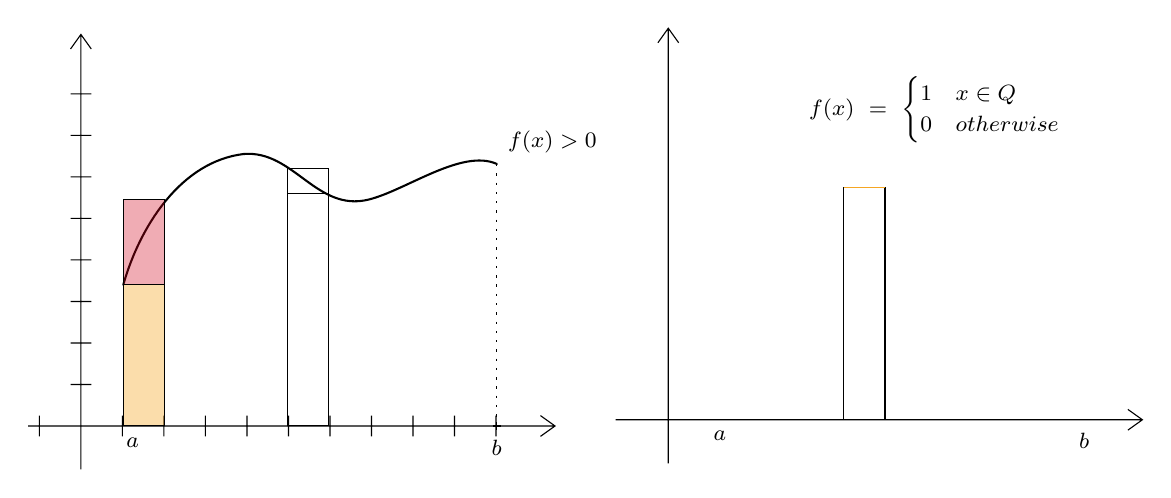
\begin{tikzpicture}[x=0.75pt,y=0.75pt,yscale=-1,xscale=1]
%uncomment if require: \path (0,300); %set diagram left start at 0, and has height of 300
\centering
%Shape: Axis 2D [id:dp5480263477292685] 
\draw  (50,241.64) -- (303.8,241.64)(75.38,53) -- (75.38,262.6) (296.8,236.64) -- (303.8,241.64) -- (296.8,246.64) (70.38,60) -- (75.38,53) -- (80.38,60) (95.38,236.64) -- (95.38,246.64)(115.38,236.64) -- (115.38,246.64)(135.38,236.64) -- (135.38,246.64)(155.38,236.64) -- (155.38,246.64)(175.38,236.64) -- (175.38,246.64)(195.38,236.64) -- (195.38,246.64)(215.38,236.64) -- (215.38,246.64)(235.38,236.64) -- (235.38,246.64)(255.38,236.64) -- (255.38,246.64)(275.38,236.64) -- (275.38,246.64)(55.38,236.64) -- (55.38,246.64)(70.38,221.64) -- (80.38,221.64)(70.38,201.64) -- (80.38,201.64)(70.38,181.64) -- (80.38,181.64)(70.38,161.64) -- (80.38,161.64)(70.38,141.64) -- (80.38,141.64)(70.38,121.64) -- (80.38,121.64)(70.38,101.64) -- (80.38,101.64)(70.38,81.64) -- (80.38,81.64) ;
\draw   ;
%Curve Lines [id:da5750477268932044] 
\draw [line width=0.75] [line join = round][line cap = round]   (95.8,173.6) .. controls (103.93,144.95) and (123.8,114.2) .. (153.8,110.6) .. controls (177.8,108.6) and (188.85,138.59) .. (213.8,132.6) .. controls (231.8,128.28) and (258.92,107.8) .. (275.8,115.4) ;
%Straight Lines [id:da7177706943638141] 
\draw  [dash pattern={on 0.84pt off 2.51pt}]  (275.8,115.4) -- (275.8,242.6) ;
%Shape: Rectangle [id:dp5408053767416018] 
\draw  [fill={rgb, 255:red, 245; green, 166; blue, 35 }  ,fill opacity=0.38 ] (95.8,241.6) -- (115.8,241.6) -- (115.8,173.6) -- (95.8,173.6) -- cycle ;
%Shape: Rectangle [id:dp3923239636084771] 
\draw  [fill={rgb, 255:red, 208; green, 2; blue, 27 }  ,fill opacity=0.33 ] (95.8,132.6) -- (115.8,132.6) -- (115.8,173.6) -- (95.8,173.6) -- cycle ;
%Shape: Rectangle [id:dp24584912849228258] 
\draw   (174.8,129.6) -- (194.8,129.6) -- (194.8,241.6) -- (174.8,241.6) -- cycle ;
%Shape: Rectangle [id:dp34691668964713374] 
\draw   (174.8,117.6) -- (194.8,117.6) -- (194.8,129.6) -- (174.8,129.6) -- cycle ;
%Shape: Axis 2D [id:dp40737828571320833] 
\draw  (333,238.64) -- (586.8,238.64)(358.38,50) -- (358.38,259.6) (579.8,233.64) -- (586.8,238.64) -- (579.8,243.64) (353.38,57) -- (358.38,50) -- (363.38,57)  ;
%Shape: Rectangle [id:dp28240967807166417] 
\draw   (442.8,126.6) -- (462.8,126.6) -- (462.8,238.6) -- (442.8,238.6) -- cycle ;
%Straight Lines [id:da2779504540997346] 
\draw [color={rgb, 255:red, 245; green, 166; blue, 35 }  ,draw opacity=1 ]   (442.8,126.6) -- (462.8,126.6) ;

% Text Node
\draw (280,98) node [anchor=north west][inner sep=0.75pt]  [font=\footnotesize] [align=left] {$\displaystyle f( x)  >0$};
% Text Node
\draw (272,247) node [anchor=north west][inner sep=0.75pt]  [font=\footnotesize] [align=left] {$\displaystyle b$};
% Text Node
\draw (96,246) node [anchor=north west][inner sep=0.75pt]  [font=\footnotesize] [align=left] {$\displaystyle a$};
% Text Node
\draw (425,72) node [anchor=north west][inner sep=0.75pt]  [font=\footnotesize] [align=left] {$\displaystyle f( x) \ =\ \begin{cases}
1 & x\in Q\\
0 & otherwise
\end{cases}$};
% Text Node
\draw (555,244) node [anchor=north west][inner sep=0.75pt]  [font=\footnotesize] [align=left] {$\displaystyle b$};
% Text Node
\draw (379,243) node [anchor=north west][inner sep=0.75pt]  [font=\footnotesize] [align=left] {$\displaystyle a$};

\draw   (273.8,241.64) -- (277.8,241.64)(275.8,239.64) -- (275.8,243.64) ;
\end{tikzpicture}

What do we really want by taking integrals?
Basically speaking, we want to find the area under the curve.
In the case of Riemann and Darboux integrals,
we partitioned the $x$-axis into subintervals,
but we encountered problems.

It's quite common that we start to try partitioning the $y$-axis instead.
We define the Lebesgue measure as
$E_{\lambda} = \left\{ x \in [a,b] | f(x) > \lambda \right\}.$

\tikzset{every picture/.style={line width=0.75pt}} %set default line width to 0.75pt        

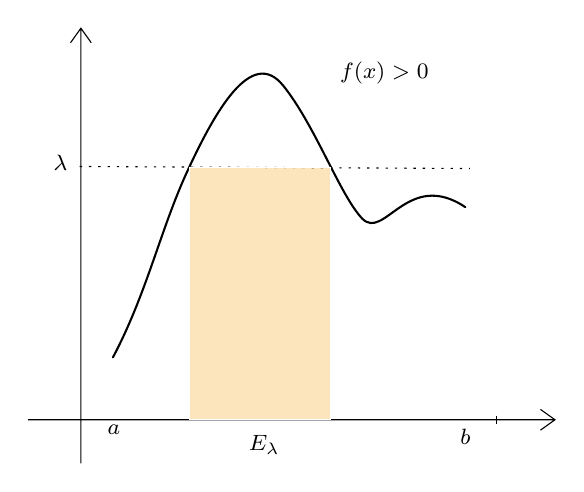
\begin{tikzpicture}[x=0.75pt,y=0.75pt,yscale=-1,xscale=1]
%uncomment if require: \path (0,300); %set diagram left start at 0, and has height of 300

%Shape: Axis 2D [id:dp7368713459977554] 
\draw  (50,241.64) -- (303.8,241.64)(75.38,53) -- (75.38,262.6) (296.8,236.64) -- (303.8,241.64) -- (296.8,246.64) (70.38,60) -- (75.38,53) -- (80.38,60)  ;
%Curve Lines [id:da47596783152208033] 
\draw [line width=0.75] [line join = round][line cap = round]   (90.8,211.6) .. controls (107.26,180.5) and (113.8,149.6) .. (126.8,121.6) .. controls (139.8,93.6) and (157.48,61.62) .. (172.8,80.6) .. controls (188.12,99.58) and (200.18,133.32) .. (210.8,144.6) .. controls (221.42,155.88) and (232.8,120.6) .. (260.6,139.2) ;
%Straight Lines [id:da5789424259496938] 
\draw  [dash pattern={on 0.84pt off 2.51pt}]  (74.8,119.6) -- (262.8,120.6) ;
%Straight Lines [id:da9105862457970941] 
\draw  [dash pattern={on 0.84pt off 2.51pt}]  (127.8,119.6) -- (127.8,241.6) ;
%Straight Lines [id:da6325422272939283] 
\draw  [dash pattern={on 0.84pt off 2.51pt}]  (195.8,119.6) -- (195.8,241.6) ;
%Shape: Rectangle [id:dp20836883762828573] 
\draw  [color={rgb, 255:red, 255; green, 255; blue, 255 }  ,draw opacity=1 ][fill={rgb, 255:red, 245; green, 166; blue, 35 }  ,fill opacity=0.3 ] (127.8,120.1) -- (195.8,120.1) -- (195.8,241.6) -- (127.8,241.6) -- cycle ;

% Text Node
\draw (257,245) node [anchor=north west][inner sep=0.75pt]  [font=\footnotesize] [align=left] {$\displaystyle b$};
% Text Node
\draw (87,243) node [anchor=north west][inner sep=0.75pt]  [font=\footnotesize] [align=left] {$\displaystyle a$};
% Text Node
\draw (61,113) node [anchor=north west][inner sep=0.75pt]  [font=\footnotesize] [align=left] {$\displaystyle \lambda $};
% Text Node
\draw (155,248) node [anchor=north west][inner sep=0.75pt]  [font=\footnotesize] [align=left] {$\displaystyle E_{\lambda }$};
% Text Node
\draw (199,68) node [anchor=north west][inner sep=0.75pt]  [font=\footnotesize] [align=left] {$\displaystyle f( x)  >0$};

\draw   (273.8,241.64) -- (277.8,241.64)(275.8,239.64) -- (275.8,243.64) ;
\end{tikzpicture}

Assuming that $E_{\lambda}$ is measurable, we know that the shaded area is $\lambda \vert E_{\lambda} \vert.$


% For our general regression model $y_i = x_i^{\prime} \beta + u_i$, we have $\mathbb{E}[x_i u_i] \neq 0$,
thus $\hat{\beta}_{OLS} \overset{\rho}{\rightarrow} \beta$ doesn't hold.

To consistently estimate $\beta$, we require additional assumptions.
One type of information which is commonly used in economics is the \textbf{instruments}.

\begin{definition}[Instrumental Variable]\label{def:IV}
    \

    We take $z_i \in \mathbb{R}^r$ as an instrumental variable if:
    \begin{align*}
        \mathbb{E}[z_i u_i] &= 0 \\
        \mathbb{E}[z_i x_i] &\neq 0 \\
        \mathbb{E}[z_i z_i^{\prime}] &> 0 \\
        \rank \Bigl(\mathbb{E}[z_i x_i^{\prime}] \Bigr) &= k \leq r \footnote{We say that the model is just-identified if $k = r$ and over-identified if $k < r$.}
    \end{align*}
\end{definition}

\subsection{Instrumental Variables and 2SLS}

Then, we have the 2SLS method:
\begin{definition}[2SLS Method]
    \ 
    \begin{enumerate}
        \item Estimate: $x_i = z_i^{\prime} \gamma + e_i \Rightarrow \hat{\gamma} = (Z^{\prime} Z)^{-1}Z^{\prime} X \Rightarrow \hat{X} = Z^{\prime} \hat{\gamma} = P_Z X$;
        \item Estimate: $y_i = \hat{x}_i^{\prime} \beta + u_i^*$.
        \begin{align*}
            \hat{\beta}_{2SLS} &= (\hat{X}^{\prime} \hat{X})^{-1}\hat{X}^{\prime} Y \\ 
            &= \left((P_Z X)^{\prime} P_Z X\right)^{-1} (P_Z X)^{\prime} Y \\ 
            &= (X^{\prime} P_Z X)^{-1} X^{\prime} P_Z Y \\
            &= \left(X^{\prime} Z (Z^{\prime} Z)^{-1} Z^{\prime} X\right)^{-1} X^{\prime} Z (Z^{\prime} Z)^{-1} Z^{\prime} Y \\ 
            &= \beta + \left(X^{\prime} Z (Z^{\prime} Z)^{-1} Z^{\prime} X\right)^{-1} X^{\prime} Z (Z^{\prime} Z)^{-1} Z^{\prime} u \\ 
            &= \beta + \left(Z^{\prime} X\right)^{-1} \left(Z^{\prime} Z\right) \left(X^{\prime} Z\right)^{-1} X^{\prime} Z \left(Z^{\prime} Z\right)^{-1}  Z^{\prime} u \footnote{To compute $\hat{\beta}_{2SLS}$, we need $Z^{\prime} Z$ to be full rank, which requires us to have more observations than IVs.} \\
            &= \beta + \left(Z^{\prime} X\right)^{-1} Z^{\prime} u \\
            % &\overset{p}{\rightarrow} \beta + Q_{xz}^{-1} \mathbb{E}[x_i z_i^{\prime}] \mathbb{E}[z_i z_i^{\prime}] \mathbb{E}[z_i u_i]\\ 
            &\overset{p}{\rightarrow} \beta.
        \end{align*}
    \end{enumerate}
\end{definition}
Ideally, $z_i$ should be as highly correlated with $x_i$ as possible, but uncorrelated with $u_i$.
To see this, we find hte variance of $\hat{\beta}_{2SLS}$
\begin{align*}
    \mathbb{V}[\hat{\beta}_{2SLS} | X, Z] &= \mathbb{V}\left[\left(X^{\prime} P_Z X \right)^{-1} X^{\prime} P_Z U | X, Z \right] \\
    &= \left(X^{\prime} P_Z X \right)^{-1} \mathbb{V}\left[X^{\prime} P_Z U | X, Z \right] \left(X^{\prime} P_Z X \right)^{-1} \\
    &= \left(X^{\prime} P_Z X \right)^{-1} X^{\prime} P_Z \mathbb{E}[U U^{\prime} | X, Z] P_Z X \left(X^{\prime} P_Z X \right)^{-1}\\
    &= \left(X^{\prime} P_Z X\right)^{-1} \sigma^2
\end{align*}
which holds under homoskedasticity.
As we know $\mathbb{V}[\hat{\beta}_{OLS}] = (X^{\prime} X)^{-1} \sigma^2$, 
\begin{align*}
    \mathbb{V}\left[\hat{\beta}_{OLS}\right]^{-1} - \mathbb{V}\left[\hat{\beta}_{2SLS} \right]^{-1} &= (\sigma^2)^{-1} X^{\prime} X - (\sigma^2)^{-1} X^{\prime} P_Z X \\
    &= (\sigma^2)^{-1} X^{\prime} (I - P_Z) X \\
    &= (\sigma^{-2}) X^{\prime} M_Z X \\
    &= \sigma^{-2} (\underset{\hat{E}}{\underbrace{M_Z X}})' M_Z X \\
    &= \sigma^{-2} SSR_{1SLS} > 0.
\end{align*}
This means that the variance of 2SLS estimator is larger than that of the OLS.

By the usual arguments, the asymptotic analysis reveals that:
\begin{gather*}
    \sqrt{n} (\hat{\beta}_{2SLS} - \beta) \overset{p}{\rightarrow} \mathcal{N} (0, V_{2SLS})
\end{gather*}
where
\begin{gather*}
    V_{2SLS}  = Q_{XZ}^{-1} X^{\prime} Z \left(Z^{\prime} Z\right)^{-1} Z^{\prime} U U^{\prime} Z \left(Z^{\prime} Z \right)^{-1} \left(X^{\prime} Z\right)^{\prime} Q_{XZ}^{-1}
\end{gather*}
where $Q_{XZ} = \left(Z^{\prime} X\right) \left(Z^{\prime} Z\right)^{-1}  \left(X^{\prime} Z\right)$

As usual, we can estimate it by replacing $u_i$ with $\hat{u}_i$ and expectation operators with population means.
Thereby, it's important to note that $u_i \neq u_i^*$, and to obtain $\hat{u}_i$, we don't use $\hat{x}_i$,but $x_i$:
\begin{gather*}
     \hat{u}_i = y_i - x_i^{\prime} \hat{\beta}_{2SLS}
\end{gather*}
Under homoskedasticity, $V_{2SLS} = \sigma^2 Q_{XZ}^{-1} $, which we estimate using $\hat{\sigma}^2 = \frac{1}{n} \sum_i u_i^2$.


\subsection{Weak Identification in IV Models}

If the the correlation between $x_i$ and $z_i$ is weak, then we say it's a \textbf{weak instrument}.
Under weak IVs, the finite sample distribution of $\hat{\beta}_{2SLS}$ may not assemble the asymptotic property.

In absence of an asymptotic distribution, we can conduct inference using its numerical approximation via bootstrapping.
Or alternatively, we can construct a confidence set for $\beta$ using the Following the procedure of Anderson and Rubin (1949).

The method is based on the idea that, for $\beta = \beta_0$, the auxiliary regression $y_i - x_i^{\prime} \beta = \delta z_i + v_i$ should yield $\delta =0$,
because $y_i - x_i^{\prime} \beta_0 = u_i$ and $u_i$ is uncorrelated with $z_i$.

\begin{theorem}[Anderson-Rubin Method]\label{thm:IV-AR}
    \
    
    For a given $\beta_0$, we get:
    \begin{gather*}
        \sqrt{n} \hat{\delta}(\beta_0) = \sqrt{n} \left(Z^{\prime} Z \right)^{-1} Z^{\prime} (Y - X \beta_0) = \left(Z^{\prime} Z\right)^{-1} \sqrt{n} Z^{\prime} U \overset{d}{\rightarrow} \mathcal{N} \left(0, \frac{\sigma_u^2}{\mathbb{E}(z_i^2)} \right)
    \end{gather*}
    which allows us to test $\mathcal{H}_0: \delta =0.$
    For many $\beta$s, test: $\mathcal{H}_0: \delta(\beta) = 0$, e.g. using t-test.
    \[T_t = \frac{\hat{\delta}(\beta_0)}{se(\hat{\delta}(\beta_0))} = \frac{\hat{\delta}_0}{\sqrt{\hat{\sigma}_u^2 / Z^{\prime} Z} } \overset{d}{\rightarrow} \mathcal{N}(0,1)\]
    The 90\% CI for $\beta$ is the set of $\beta$s at which $\delta(\beta) = 0$ cannot be rejected at 90\% confidence level.
    A confidence set for $\beta$ is given by taking all $\beta_0$ such that $\mathcal{H}_0: \delta =0$ cannot be rejected.
\end{theorem}

\begin{remark}[About Anderson-Rubin (AR) Test]\footnote{Retrieved from MIT14.384 Time Series Analysis, Fall 2007
    Professor Anna Mikusheva, Lecture 7-8, \url{https://ocw.mit.edu/courses/14-384-time-series-analysis-fall-2013/365cba34145fa204731e9df202d4771e_MIT14_384F13_lec7and8.pdf}}
    \
    
    Consider our model
    \begin{align*}
        y&=X\beta+u,\\
        X&=Z\Pi+v,
    \end{align*}
    where $X$ is one-dimensional and test for hypothesis $H_0:\beta=\beta_0.$ Under the null, vector $y-X\beta$ is equal to
    the error $u_t$ and is uncorrelated with $Z$ (due to exogeneity of instruments). 
    The suggested statistics is:
    \begin{gather*}
        AR(\beta_0)=\frac{(y-X\beta)'P_Z(y-X\beta)}{(y-X\beta)'M_Z(y-X\beta)/(T-k)}.
    \end{gather*}
    here $P_Z=Z(Z^{\prime}Z)^{-1}Z^{\prime}, M_Z=I-P_z.$
    
    The distribution of AR does not depend on $\mu$ asymptotically $AR\to\chi_k^2/k.$ The formula may remind you of the J-test for over-identifying restrictions. It would be a J-test if one were to plugs in $\hat{\beta}_{TSLS}.$
    In a more general situation of more than one endogenous variable and/or included exogenous regressors AR statistic is F-statistic testing 
    that all coeffcients on $Z$ are zero in the regression of $y-\beta_0X$ on $Z$ and $W$.
    
    Note, that one tests all coefficients $\beta$ simultaneously (as a set) in a case of more than one endogenous regressor.
    AR confidence set One can construct a confidence set robust towards weak instruments based on the AR test by inverting it. 
    That is, by finding all $\beta$ which are not rejected by the data. In this case, it is the set :
    \begin{gather*}
        CI =\{ \beta_0:AR(\beta_0)<\chi_{k,1-\alpha}^2 \}.
    \end{gather*}
    The nice thing about this procedure is that solving for the confidence set is equivalent to solving a quadratic inequality. 
    This confidence set can be empty with positive probability (caution!).
\end{remark}
% \chapter{Causal Inference}
% Rubin (1975\cite{rubin1975bayesian}) and Holland (1986\cite{holland1986statistics}) made up the aphorism\cite{ding2023causalinference}:
\begin{quote}
  \textit{``No causation without manipulation''}
\end{quote}
Not everybody agrees with this point of view.

In our lectuere, we'll define causal effects using the potential outcomes framework
(Neyman, 1923\cite{neyman1923experiment}; Rubin, 1974\cite{rubin1974estimating}).


\section{Potential Outcomes Framework}

In this framework, an experiment, or at least a thought experiment, 
has a treatment, and we are interested in its effect on an outcome 
or multiple outcomes. Sometimes, the treatment is also called an
intervention or a manipulation.

Firstly, we consider an experiment with $n$ units indexed by $i=1, 2, \cdots, n$.
We focus on a treatment with two levels:
\begin{gather*}
  d_i = \left\{\begin{matrix}
    0 & \text{control}\\
    1 & \text{treatment}
  \end{matrix} \right.
\end{gather*}

We seek to identify the causal effect of treatment $d_i$ on some outcome $y_i$.
For each $i$, the outcome od interest $y_i$ has two versions:
\begin{gather*}
  y_i = \left\{\begin{matrix}
    y_{0i} & d_i=0\\
    y_{1i} & d_i=1
  \end{matrix} \right.
\end{gather*}
This notation emphasizes that $y_{di}$ is the realization of the outcome $y_i$ that would materialize if unit $i$
received treatment $d_i = d$.

Neyman (1923\cite{neyman1923experiment}) first used this notation. It seems intuitive but has some hidden
assumptions. Rubin (1980\cite{rubin1980comment}) made the following clarifications on the hidden assumptions.
\begin{assumption}[No interference]\label{assumption:no_interference}
  \

  Unit $i$'s potential outcomes do not depend on other units' treatments. 
  This is sometimes called the no-interference assumption.
\end{assumption}
\begin{assumption}[Consistency]\label{assumption:consistency}
  \

  There are no other versions of the treatment. 
  Equivalently, we require that the treatment levels be well-defined, 
  or have no ambiguity at least for the outcome of interest. 
  This is sometimes called the consistency assumption.
\end{assumption}

The causal effect of the treatment on the $i$-th unit is then defined as:
\begin{gather*}
  \Delta_i = y_{1i} - y_{0i} 
\end{gather*}
These potential outcomes are constants at the level of unit $i$.

\begin{remark}[Problem of causal inference]
  \

  The fundamental problem in causal inference is that only one treatment can be assigned to a given individual, 
  and so only one of $y_{0i}$ and $y_{1i}$ can be observed. Thus $\Delta_i$ can never be observed.
\end{remark}

\begin{definition}[Stable Unit Treatment Value Assumption (SUTVA)]
\label{def:sutva}
  \

  Rubin (1980\cite{rubin1980comment}) called the Assumptions \ref{assumption:no_interference} and \ref{assumption:consistency} above together 
  the \textit{Stable Unit Treatment Value Assumption (SUTVA).}
\end{definition}
In principle, by virtue of being (discrete) RVs, both $d_i$ and $y_i$ each have a distribution function,
which, together with their possible realizations, defines various moments.
However, their unconditional probabilities and moments at the level of unit $i$ is not of interest.
Only the conditional probabilities of $y_i$ given $d_i$ is of interest.

\begin{remark}[Rubin (2005\cite{rubin2005causal})]
  \

  Under SUTVA, Rubin (2005) called the $n \times 2$ matrix of potential outcomes the Science Table:
  $$\begin{array}{ccc}
  \hline
  i & y_{1i}  & y_{0i}  \\
  \hline
  1 & y_{11}  & y_{01}  \\
  2 & y_{12}  & y_{02}  \\
  \vdots & \vdots & \vdots \\
  n & y_{1n}  & y_{0n} \\
  \hline
  \end{array}$$
  Due to the fundamental contributions of Neyman and Rubin to statistical causal inference, the potential outcomes framework is sometimes referred to as the Neyman Model, 
  the Neyman-Rubin Model, or the Rubin Causal Model.
  Causal effects are functions of the Science Table. Inferring individual causal effects
  $$\tau_i = y_{1i}  - y_{0i} , \quad (i=1,\ldots,n)$$
  is fundamentally challenging because we can only observe either $y_{1i} $ or $y_{0i}$,
  for each unit $i$, that is, we can observe only half of the Science Table.
\end{remark}

SUTVA(\ref{def:sutva}) ensures that the individual treatment effect is well defined.

For a population, we know that $\mathbb{E}[d_i], \mathbb{E}[y_i], \mathbb{E}[y_{0i}], \mathbb{E}[y_{1i}]$ exist,
we can define the treatment conditional expectations:
\[\mathbb{E}[y_i | d_i=1], \mathbb{E}[y_{0i} | d_i=1 ], \mathbb{E}[y_{1i} | d_i=1 ] = \mathbb{E}[y_i | d_i=1]\]
that denote the averages of the outcome $y_i$.

Analogously, we can define the control conditional expectations:
\[\mathbb{E}[y_i | d_i=0], \mathbb{E}[y_{0i} | d_i=0 ] = \mathbb{E}[y_i | d_i=0], \mathbb{E}[y_{1i} | d_i=0 ]\]
for the non-treated subpopulation.

Then, we candefine the Average Treatment Effect (ATE), the Average Treatment Effect for the Treatment-Group (ATT) and the Average
Treatment Effect for the Control-Group (ATC) as distinct objects:
\begin{align*}
  \text{ATE} &= \mathbb{E}[y_{1i}- y_{0i}]\\
  \text{ATT} &= \mathbb{E}[y_{1i}- y_{0i} | d_i=1]\\
  \text{ATC} &= \mathbb{E}[y_{1i}- y_{0i} | d_i=0]
\end{align*}
\[\mathbb{E}[z] = \mathbb{E}[z|d=1] \mathbb{P}[d=1] + \mathbb{E}[z|d=0] \mathbb{P}[d=0] = \mathbb{E}[\mathbb{E}[z|d]].\]

For sample, $\{d_i, y_i\}_{i=1}^n = \{d_i, y_{d_{i}, i}\}_{i=1}^n$, because
$y_i = y_{1i} d_i + y_{0i} (1 - d_i)$.

$N = \{i=1,2,\cdots, n\}$, $N_1 = \{i \in N: d_i = 1\} \leftarrow n_1 = \vert N_1 \vert $, $N_0 = \{i: d_i = 0\} \leftarrow n_0 = \vert N_0 \vert $.
\begin{align*}
  \frac{1}{n_1} \sum_{i \in N_1} y_i &= \frac{1}{n_1} \sum_{i \in N_1} y_{1i} \overset{p}{\rightarrow} \mathbb{E}[y_{1i} | d_i=1] = \mathbb{E}[y_i | d_i=1]\\
  \frac{1}{n_0} \sum_{i \in N_0} y_i &= \frac{1}{n_0} \sum_{i \in N_0} y_{0i} \overset{p}{\rightarrow} \mathbb{E}[y_{0i} | d_i=0] = \mathbb{E}[y_i | d_i=0]
\end{align*}
\[\frac{1}{n_1} \sum_{i \in N_1} y_i - \frac{1}{n_0} \sum_{i \in N_0} y_i \overset{p}{\rightarrow} \mathbb{E}[y_{1i} | d_i = 1] - \mathbb{E}[y_{0i} | d_i = 0] = \text{ATE} = \text{ATT} = \text{ATC}.\]

We define teh difference of treated and non-treated as: \textit{Naive Difference}.
\begin{align*}
  \text{ND} &= \mathbb{E}[y_{1i} | d_i = 1] - \mathbb{E}[y_{0i} | d_i = 0]\\
  &= \mathbb{E}[y_{1i} | d_i = 1] - \mathbb{E}[y_{0i} | d_i = 1] + \mathbb{E}[y_{0i} | d_i =1] - \mathbb{E}[y_{0i} | d_i = 0] \\
  &= ATT + \mathbb{E}[y_{0i} | d_i = 1] - \mathbb{E}[y_{0i} | d_i = 0]
\end{align*}

For LRM, $y_i = \beta_0 + \beta_1 d_i + u_i$,
\begin{align*}
  \text{ND} &= \mathbb{E}[y_i | d_i = 1] - \mathbb{E}[y_i | d_i = 0]\\
  &= \mathbb{E}[\beta_0 + \beta_1 + u_i | d_i = 1] - \mathbb{E}[\beta_0 + u_i | d_i = 0]\\
  &= \beta_1 + \mathbb{E}[u_i | d_i = 1] - \mathbb{E}[u_i | d_i = 0]  
\end{align*}



\[
\{Y_d\} \perp\!\!\!\perp D \mid X \implies \{Y_d\} \perp\!\!\!\perp D \mid \pi(X), \quad D \perp\!\!\!\perp X \mid \pi(X)
\]
% \chapter{Panel Data Analysis}
% Economists traditionally use the term \textbf{panel data} to refer to data structures consisting of observa-
tions on individuals for multiple time periods. 
There are several distinct advantages of panel data relative to cross-section data:
\begin{enumerate}
  \item Possibility of controlling for unobserved time-invariant endogeneity without the use of instrumental variables
  \item Possibility of allowing for broader forms of heterogeneity
  \item Modeling dynamic relationships and effects
\end{enumerate} 

It's typical to index observations by both the individual $i$ and the time period, $t$,
thus $y_{it} $ denotes a variable for indivual $i$ in time $t$, where $n=1, \cdots, N$, $t=1, \cdots, T.$

\begin{definition}[Balanced and Unbalanced Panel Data\cite{hansen2022econometrics}]
  \

  When observations are available on all individuals for the same time periods we say that the panel is \textbf{balanced}. 
  In this case there are an equal number $T$ of observations for each individual and the total number of observations is $n = NT$.

  When different time periods are available for the individuals in the sample we say that the panel is \textbf{unbalanced}. 
  This is the most common type of panel data set. 
  It does not pose a problem for applications but does make the notation cumbersome and also complicates computer programming.
\end{definition}

\section{Incidental Parameters Problem}

\subsection{Pooled OLS Estimation}\label{sec:POLS}

Suppose we are estimating the following panel data regression:
\begin{align*}
  y_{it} &= \alpha +x_{it}^{\prime} \beta +u_{it}, \quad \mathbb{E}[u_{it} x_{it}] = 0, \quad \mathbb{V}[u_{it} | x_{it}] = \sigma^2
\end{align*}

Omitting the distinction between intercept and slope, we can write the model as:
\begin{gather*}
  y_{it} = \tilde{x}_{it}^{\prime} \tilde{\beta} + u_{it} \\
  \tilde{x}_{it} = \begin{bmatrix}
    1 \\
    x_{it}
  \end{bmatrix}, \quad
  \tilde{\beta} = \begin{bmatrix}
    \alpha \\
    \beta
  \end{bmatrix}
\end{gather*}
where $i=1:n$, $T=1:t$.

Or, we can write the model as: 
\[ 
\underset{T\times 1}{y_i} = \underset{T \times K}{\tilde{X}_i} \underset{K \times 1}{\tilde{\beta}} + \underset{T \times 1}{u_i}
\]
Using OLS method to estimate $\tilde{\beta}$, we have:
\[
\underset{\tilde{\beta}}{\min} \sum_i \sum_t u_{it}^2 = \underset{\tilde{\beta}}{\min} \sum_i u_i^{\prime} u_i = \underset{\tilde{\beta}}{\min} (y_i - \tilde{X}_i \tilde{\beta})^{\prime} (y_i - \tilde{X}_i \tilde{\beta})
\]
The FOC of this equation is:
\begin{align*}
  \sum_i -\tilde{X}_i^{\prime} (y_i - \tilde{X}_i \tilde{\beta}) &= 0 \\
  \left(\sum_i \tilde{X}_i^{\prime} \tilde{X}_i \right) \tilde{\beta} &= \sum_i \tilde{X}_i^{\prime} y_i \\
  \hat{\tilde{\beta}}_{POLS} &= \left(\sum_i \tilde{X}_i^{\prime} \tilde{X}_i \right)^{-1} \sum_i \tilde{X}_i^{\prime} y_i \\
  &= \left(\sum_i \sum_t \tilde{x}_{it} \tilde{x}_{it}^{\prime} \right)^{-1} \left( \sum_i \sum_t \tilde{x}_{it} y_{it} \right) \\
  &= \tilde{\beta} + \left(\frac{1}{n} \sum_i \sum_t \tilde{x}_{it} \tilde{x}_{it}^{\prime} \right)^{-1} \left( \sum_i \sum_t \tilde{x}_{it} u_{it} \right) \\
  & \overset{p}{\rightarrow} \tilde{\beta} + \mathbb{E}\left[\sum_t \tilde{x}_{it} \tilde{x}_{it}^{\prime} \right] \mathbb{E}\left[\sum_t \tilde{x}_{it} u_{it} \right] \\
  &= \tilde{\beta}
\end{align*}
Hence $\hat{\beta}_{OLS}$ is consistent provided that $x_{it}$ and $u_{it}$ are contemperaneously uncorrelated,
as $\mathbb{E}[x_{it} u_{it}] = 0, \forall t.$
The regressors are allowed to be correlated with the past, and future $u_{it}$.
This occurs when there's feedback loop by which $y_{i,t-1}$ affects $x_{it}$.

In this proof, we show that either $N \to \infty $ or $T \to  \infty $ is sufficient for consistency of $\hat{\beta}_{POLS}$.
However, most panel data applications have a large $n$ and small $T$ dimension, so standrad panel data
features $T$ fixed and $n \to \infty $.

\subsection{Asymptotic Normality}

From the analysis of consistency, we know that:
\[ 
\hat{\tilde{\beta}}_{POLS}  = \left(\sum_i \tilde{X}_i^{\prime} \tilde{X}_i \right)^{-1} \sum_i \tilde{X}_i^{\prime} y_i
\]
Hence:
\begin{align*}
    \sqrt{n} (\hat{\tilde{\beta}}_{POLS}  - \tilde{\beta}) &= \left(\frac{1}{n} \sum_i \tilde{X}_i^{\prime} \tilde{X}_i \right)^{-1} \left(\frac{1}{\sqrt{n} } \sum_i \tilde{X}_i^{\prime} u_i \right) \\
    & \overset{p}{\rightarrow}\mathbb{E}[\tilde{X}_i^{\prime} \tilde{X}_i]^{-1} \overset{d}{\rightarrow} \mathcal{N}\left(0, \mathbb{E}\left[\left(\tilde{X}_i^{\prime} u_i\right) \left(\tilde{X}_i^{\prime} u_i\right)^{\prime} \right] \right)\\
    & \overset{d}{\rightarrow} \mathcal{N} \left(0, \mathbb{E}\left[\tilde{X}_i^{\prime} \tilde{X}_i \right]^{-1} \mathbb{E}\left[\tilde{X}_i^{\prime} u_i u_i^{\prime} \tilde{X}_i \right] \mathbb{E}\left[\tilde{X}_i^{\prime} \tilde{X}_i \right] \right)
\end{align*}


The above model is homogeneous, which is unattractive, as the data generating process would 
differ across $i$, with some units having a higher level of the outcome variable $y_{it} $
than others, regardless of covariates $x_{it}$(with a higher intercept $\alpha$) or a stronger effect
of some covariates $x_{it, k} $ on $y_{it}$ than others.

At the other extreme, we assume the fully heterogenous estimation:
\[y_{it} = \alpha_i + x_{it}^{\prime} \beta + u_{it}, \quad \mathbb{E}[u_{it} x_{it}] = 0, \quad \mathbb{V}[u_{it} | x_{it}] = \sigma_i^2. \]

Under $T=1$, we run $y_i = \beta_0 + x_i^{\prime} \beta + v_i$, 
where $v_i = u_i + \underset{\tilde{\alpha}_i}{\underbrace{\alpha_i - \beta_0}}$
and $\mathbb{E}[v_i] = 0$.

Under $T>1$, we run:
\begin{align*}
    y_i &= x_i^{\prime} \beta  + \sum_{j=1}^{n} \alpha_j \mathbf{1}\{i=j\} + u_{it} \\
    &= \tilde{x}_{it}^{\prime} \tilde{\beta} + u_{it} \\
    \tilde{x}_{it} &= \begin{bmatrix}
      x_{it} \\
      \mathbf{1}\{i=1\} \\
      \mathbf{1}\{i=2\} \\
      \vdots \\
      \mathbf{1}\{i=n\}
    \end{bmatrix}, \quad
    \tilde{\beta} = \begin{bmatrix}
      \beta \\
      \alpha_1 \\
      \alpha_2 \\
      \vdots \\
      \alpha_n
    \end{bmatrix}
\end{align*}

In a similar way, we can write the regression as
\[y_{i}  = \tilde{X}_i \tilde{\beta}_i + u_i \]
with $\tilde{\beta}_i$ is specific for each $i$.
We have $n$ separate time series regressions, one for each unit $i$. 

Following the same analyzing process, we can get:
\[
\hat{\tilde{\beta}}_{i,OLS} = \Bigl( \sum_i \tilde{X}_i^{\prime} \tilde{X}_i \Bigr) \sum_i \tilde{X}_i^{\prime} y_i = \Bigl( \sum_t \tilde{x}_{it} \tilde{x}_{it}^{\prime} \Bigr)^{-1} \Bigl( \sum_t \tilde{x}_{it} y_{it} \Bigr),
\]
which obviously shows that $\hat{\tilde{\beta}}$ is consistent $\operatorname{\iff}$ $T \rightarrow\infty $.

\subsection{One-way error component model}\label{sec:one-way error component model}
With the fully homogeneous specification unattractive and the fully heterogeneous specifi-
cation infeasible, researchers usually go for a compromise and let intercepts (and error term
variances) be unit-specific.

\begin{definition}[One-way error component model]
  \begin{equation}
    y_{it}  = \alpha_i + x_{it}^{\prime} + u_{it}, \quad \mathbb{E}[u_{it} x_{it}] = 0, \quad \mathbb{V}[u_{it} | x_{it}] = \sigma^2, \label{eq: basic model}
  \end{equation}
where $\alpha_i$ is an individual-specific effect, and $u_{it}$ are idiosyncratic(i.i.d.) errors.
\end{definition}

In any case, the equation above makes clear that $\alpha_i $ contains all factors that affect $y_{it}$, that are
not included in $x_{it}$ and that are fixed over time (the time-varying factors are in $u_{it}$).

Suppose hte model is correctly specified, and we have a cross-sectional detaset available, i.e. $T=1$.
Then, we would estimate:
\[y_{it} = \beta_0 + x_{it}^{\prime} + v_i, \text{ for} t=1,\]
where $v_i = \alpha_i + u_{it} -\beta_0.$

If the unobserved heterogeneity $\alpha_i$ is correlated with the covariate $x_{it} $,
our standard OLS estimator is biased and inconsistent.

If we have a panel dataset, i.e. $T>1$, we can write the above model into a regression of $k+n$ regressors:
\[
y_{it} = x_{it}^{\prime} \beta + \sum_{j=1}^{n}\mathbf{1}\{i=j\} \alpha_j + u_{it} = x_{it}^{*^{\prime}} \beta^* + u_{it},
\]
where $x_{it}^* = \Bigl( x_{it}^{\prime}, \mathbf{1}\{i=1\}, \cdots, \mathbf{1}\{i=n\} \Bigr)^{\prime} $,
and $\beta^* = \Bigl( \beta^{\prime}, \alpha_1, \cdots, \alpha_n \Bigr)^{\prime}.$

This leads to the pooled OLS estimator for $\beta^*$:
\[
\hat{\beta}^* = \Bigl( \sum_i \sum_t x_{it}^* x_{it}^{*^{\prime}} \Bigr) \sum_i \sum_t x_{it}^* y_{it}. 
\]

However, the estimator suffers from the so-called \textbf{IPP problem}, 
as the number of parameters increase with $n \rightarrow\infty $, 
the limit of $\frac{1}{n} \sum_i x_{it}^* x_{it}^{*^{\prime}}$ is not well-defined
and as a result, we can't establish consistency of $\hat{\beta}_{OLS}.$
% \section{Random Effects}

As with pooled OLS, a random effects analysis puts $\alpha_i$ into the error term.
In fact, random effects analysis imposes more assumptions than those needed for pooled OLS:
\textbf{strict exogeneity} in addition to orthogonality between $\alpha_i$ and $x_{it}$. 

\subsection{Basic Assumptions and POLS}

Stating the assumption in terms of conditional means, we have:
\begin{assumption}[Random Effect]\label{assumption:RE}
    \

    \begin{enumerate}
        \item[(a)] $\mathbb{E}[u_{it} | X_i, \alpha_i] = 0, \forall t.$
        \item[(b)] $\mathbb{E}[\alpha_i | X_i] = \mathbb{E}[\alpha_i] = 0.$
    \end{enumerate}
    where $X_i = (x_{i1}, \cdots, x_{iT})$.
\end{assumption}
Assumption \ref{assumption:RE}(a) is the strict exogeneity condition and Assumption \ref{assumption:RE}(b) is is how we will state the orthogonality.

\begin{remark}[Why Strict Ecogeneity?\cite{wooldridge2010econometric}]
    \

    Why do we maintain Assumption \ref{assumption:RE}(a) when it is more restrictive than needed for
    a pooled OLS analysis? Because the random e¤ects approach exploits the serial correlation in
    the composite error, $v_{it} = \alpha_i + u_{it}$, in a generalized least squares (GLS) framework. In
    order to ensure that feasible GLS is consistent, we need some form of strict exoge-
    neity between the explanatory variables and the composite error.

    Under this assumption, we can write:
    \begin{align*}
        & y_{it} = x_{it}^{\prime} \beta + v_{it} \\
        & \mathbb{E}[v_{it} | X_i] = 0, t=1, \cdots, T
    \end{align*}
    The conditions shows that our model satisfies the GLS assumption, which confirms that
    we can apply GLS methods that account for the particular error structure $v_{it} = \alpha_i + u_{it}.$
\end{remark}


By defining $v_{it} = u_{it} + \alpha_i - \beta_0$, we can transform the random effect model to the following:
\begin{align*}
    y_{it} &= \alpha_i + x_{it}^{\prime} \beta + u_{it} \\
    &= \underset{\tilde{x}_{it}^{\prime}}{\underbrace{\beta_0 + x_{it}^{\prime}\beta}} + \underset{\equiv v_{it}}{\underbrace{u_{it} + \alpha_i - \beta_0}}
\end{align*}
Defining again $\tilde{x}_{it} = (1, x_{it}^{\prime})^{\prime}$, $\tilde{\beta} = (\beta_0, \beta^{\prime})^{\prime}$, we can rewrite the model as:
\begin{align*}
    y_{it} &= \tilde{x}_{it}^{\prime} \beta + v_{it} \Leftrightarrow y_i = \tilde{X}_i^{\prime} \tilde{\beta} + v_i \\
    \rightarrow \hat{\tilde{\beta}} &= \left(\sum_i \tilde{X}_i^{\prime} \tilde{X}_i \right)^{-1} \sum_i \tilde{X}_i^{\prime} y_i
\end{align*}

With this intercept $beta_0$, $\mathbb{E}[v_i] = 0$ is guaranteed to hold.
Define $\tilde{\alpha}_i = \alpha_i - \beta_0$ as the mean-zero unit-specific heterogenety so that $v_i = u_i + \tilde{\alpha}_i.$


\begin{note}[POLS]
    \

    Homogenous spec: $y_{it} = \alpha  + x_{it}^{\prime} \beta + u_{it} = \tilde{x}_{it}^{\prime} \tilde{\beta} + v_{it}.$
    $\hat{\tilde{\beta}}$ is consistent if $\mathbb{E}[v_{it} x_{it}]=0, \forall t.$
\end{note}
Using pooled OLS to estimate $\hat{\tilde{\beta}}$,
\begin{align*}
    \hat{\tilde{\beta}}_{RE-OLS/POLS} &= \left(\frac{1}{n} \sum_i \tilde{X}_i^{\prime} \tilde{X}_i \right)^{-1} \frac{1}{n} \sum_i \tilde{X}_i^{\prime} y_i \\
    &= \tilde{\beta} + \left(\frac{1}{n} \sum_i \tilde{X}_i^{\prime} \tilde{X}_i \right)^{-1} \frac{1}{n} \sum_i \tilde{X}_i^{\prime} v_i \\
    &\overset{p}{\rightarrow} \tilde{\beta} + \mathbb{E}[\tilde{X}_i^{\prime} \tilde{X}_i]^{-1} \mathbb{E}[\tilde{X}_i^{\prime} v_i] \\
    \text{where} \quad \mathbb{E}[\tilde{X}_i^{\prime} v_i] &= \mathbb{E}\left[\sum_t \tilde{x}_{it}^{\prime} v_{it} \right] \\
    &= \sum_t \mathbb{E}\left[\tilde{x}_{it}^{\prime} v_{it}  \right] \\
    &= \sum_t \mathbb{E}\left[\tilde{x}_{it}(u_{it} + \alpha_i - \beta_0)\right]
\end{align*}
Here, the error term $v_i$ is not equal to the original error term $u_{it}$.
\begin{note}
    \

    Under the random effect, you have to use the heteroskedasticity-robust methods.
    Because even if we assume $u_{it}$ to be homoskedastic, $v_{it}$ is not,
    as it includes also the unit-specific heterogeneity $\alpha_i$.
\end{note}

\subsection{From POLS to GLS}

So, to obtain consistency, we need to assume that:
\begin{itemize}
    \item $\mathbb{E}[u_{it} | \tilde{x}_{it}, \tilde{\alpha}_i] = 0, \forall t$.
    \item $\mathbb{E}[\tilde{\alpha_i} | \tilde{x}_{it}] = 0, \forall t$.
\end{itemize}
And, we are also obliged to use HAC-robust standard error because:
\[\Omega \equiv \mathbb{E}[v_i v_i^{\prime} | \tilde{X}_i] = \mathbb{E}[(\alpha_i \mathbf{1}_i + u_i)(\tilde{\alpha}_i \mathbf{1}_i + u_i)^{\prime} | \tilde{X}_i] = \mathbb{E}[\tilde{\alpha}_i^2 \mathbf{1}_i \mathbf{1}_i^{\prime} | \tilde{X}_i] + \mathbb{E}[u_i u_i'| \tilde{X}_i] \]
is not diagonal.

\begin{assumption}[Random Effect]\label{assumption:RE2}
    \

    $\rank \mathbb{E}\left[X_i^{\prime} \Omega^{-1} X_i \right] = K$
\end{assumption}
We know that both GLS and feasible GLS estimator would be consistent under Asusmption \ref{assumption:RE} and \ref{assumption:RE2}.
A general FGLS analysis, using an unrestricted variance estimator $\Omega$,
is consistent and asymptotically normal as $N \to \infty.$

But, we won't exploit the unobserved effects structure $v_{it}.$
A standard random e¤ects analysis adds assumptions on the idiosyncratic errors that
give $\Omega$ a special form. The first assumption is that the idiosyncratic errors
$u_{it}$ have a constant unconditional variance across $t$:
\begin{assumption}[RE-Homoskedasticity]\label{assumption:RE-homoskedasticity}
    \

    $\mathbb{E}[u_{it}^2] = \sigma_u^2, \forall t$
\end{assumption}
The second assumption is that the idiosyncratic errors are serially uncorrelated:
\begin{assumption}[RE-Serial Uncorrelated]\label{assumption:RE-serial_uncorrelated}
    \

    $\mathbb{E}[u_{it} u_{is}] = 0, \forall t \neq s$
\end{assumption}
Under these two assumptions, we can derive the variances and covariances of the
elements of $v_i$.
Given the error structure the natural estimator for $\beta$ is GLS. The GLS eimator for $\beta$ is:
\begin{gather*}
    \hat{\tilde{\beta}}_{RE-GLS} = \left( \sum_i \tilde{X}_i^{\prime} \Omega^{-1} \tilde{X}_i \right)^{-1} \sum_i \tilde{X}_i^{\prime} \Omega^{-1} y_i
\end{gather*}
where $\Omega ^{-\frac{1}{2}} y_i = \Omega ^{-\frac{1}{2}} \tilde{X}_i^{\prime} \tilde{\beta} + \Omega^{-\frac{1}{2}}v_i.$
\begin{align*}
    \Omega &= \mathbb{E}[v_i v_i^{\prime} | \tilde{X}_i] = \mathbb{E}\left[ \begin{bmatrix}
        v_{i1} \\
        v_{i2} \\
        \vdots \\
        v_{iT}
    \end{bmatrix} \begin{bmatrix}
        v_{i1} & v_{i2} & \cdots & v_{iT}
    \end{bmatrix} | \tilde{X}_i \right]\\
    &= \mathbb{E}\begin{bmatrix}
        \mathbb{E}[v_{i1}^2 | \tilde{X}_i] & \mathbb{E}[v_{i1}v_{i2} | \tilde{X}_i] & \cdots & \mathbb{E}[v_{i1}v_{iT} | \tilde{X}_i] \\
        \mathbb{E}[v_{i2}v_{i1} | \tilde{X}_i] & \mathbb{E}[v_{i2}^2 | \tilde{X}_i] & \cdots & \mathbb{E}[v_{i2}v_{iT} | \tilde{X}_i] \\
        \vdots & \vdots & \ddots & \vdots \\
        \mathbb{E}[v_{iT}v_{i1} | \tilde{X}_i] & \mathbb{E}[v_{iT}v_{i2} | \tilde{X}_i] & \cdots & \mathbb{E}[v_{iT}^2 | \tilde{X}_i]
    \end{bmatrix} \\
    &= \begin{bmatrix}
        \mathbb{E}\left[\alpha_i^2 | \tilde{X}_i \right] + \mathbb{E}[u_{i1}^2 | \tilde{X}_i] & \mathbb{E}\left[\alpha_i^2 | \tilde{X}_i \right] + \mathbb{E}[u_{i1}u_{i2} | \tilde{X}_i] & \cdots & \mathbb{E}\left[\alpha_i^2 | \tilde{X}_i \right] + \mathbb{E}[u_{i1}u_{iT} | \tilde{X}_i] \\
        \mathbb{E}\left[\alpha_i^2 | \tilde{X}_i \right] + \mathbb{E}[u_{i2}u_{i1} | \tilde{X}_i] & \mathbb{E}\left[\alpha_i^2 | \tilde{X}_i \right] + \mathbb{E}[u_{i2}^2 | \tilde{X}_i] & \cdots & \mathbb{E}\left[\alpha_i^2 | \tilde{X}_i \right] + \mathbb{E}[u_{i2}u_{iT} | \tilde{X}_i] \\
        \vdots & \vdots & \ddots & \vdots \\
        \mathbb{E}\left[\alpha_i^2 | \tilde{X}_i \right] + \mathbb{E}[u_{iT}u_{i1} | \tilde{X}_i] & \mathbb{E}\left[\alpha_i^2 | \tilde{X}_i \right] + \mathbb{E}[u_{iT}u_{i2} | \tilde{X}_i] & \cdots & \mathbb{E}\left[\alpha_i^2 | \tilde{X}_i \right] + \mathbb{E}[u_{iT}^2 | \tilde{X}_i]
    \end{bmatrix}\\
    &= \begin{bmatrix}
        \sigma_u^2 + \sigma_{\alpha}^2 & \sigma_{\alpha}^2 & \cdots & \sigma_{\alpha}^2 \\
        \sigma_{\alpha}^2 & \sigma_u^2 + \sigma_{\alpha}^2 & \cdots & \sigma_{\alpha}^2 \\
        \vdots & \vdots & \ddots & \vdots \\
        \sigma_{\alpha}^2 & \sigma_{\alpha}^2 & \cdots & \sigma_u^2 + \sigma_{\alpha}^2
    \end{bmatrix} \\
    &= \sigma_{\alpha}^2 \mathbf{1}_i \mathbf{1}_i^{\prime} + \sigma_u^2 I \\
    \text{beacuse } &\mathbb{V}[\tilde{\alpha}_i|\tilde{X}_i] = \sigma_{\alpha_i}^2 = \sigma_{\alpha}^2 \\
    &\mathbb{V}[u_{it} | \tilde{X}_i] = \sigma_u^2, \forall i.
\end{align*}
where $I$ is an identity matrix of dimention $T_i$.
Under the assumption $\mathbb{E}[u_{it} x_{is}] = 0$, we now describe some statistical properties of $\hat{\tilde{\beta}}_{RE-GLS}.$

\subsubsection{RE Consistency}
\begin{align*}
    \hat{\tilde{\beta}}_{RE-GLS} - \tilde{\beta} &= \Bigl( \sum_i \tilde{X}_i^{\prime} \Omega^{-1} \tilde{X}_i \Bigr)^{-1} \Bigl( \sum_i \tilde{X}_i^{\prime} \Omega^{-1} v_i \Bigr) \\
    & \rightarrow \mathbb{E}\Bigl[ \sum_i \tilde{X}_i^{\prime} \Omega^{-1} \tilde{X}_i \Bigr] \mathbb{E}\Bigl[ \sum_i \tilde{X}_i^{\prime} \Omega^{-1} v_i \Bigr] \\
    \text{where } \mathbb{E}\Bigl[ \sum_i \tilde{X}_i^{\prime} \Omega^{-1} v_i \Bigr] &= \sum_i \mathbb{E}\Bigl[ \tilde{X}_i^{\prime} \Omega^{-1} v_i \Bigr] \\
    &= \sum_i \tilde{X}_i^{\prime} \Omega^{-1} \mathbb{E}[v_i | \tilde{X}_i] \\
    &= \sum_i \tilde{X}_i^{\prime} \Omega^{-1} \mathbb{E}[u_i + \tilde{\alpha}_i | \tilde{X}_i] \\
    &=0
\end{align*}
Thus, $\hat{\tilde{\beta}}_{RE-GLS} $ is conditionally unbiased for $\tilde{\beta}$.
The conditional variance of $\hat{\tilde{\beta}}_{RE-GLS}$ is:
\begin{align*}
    \mathbb{V}\Bigl[\hat{\tilde{\beta}}_{RE-GLS}\Bigr] = \Bigl( \sum_i \tilde{X}_i^{\prime} \Omega^{-1} \tilde{X}_i \Bigr)^{-1} \sigma_{u}^2
\end{align*}

\subsubsection{RE Asymptotic Distribution}
The asymptotic variance of $\hat{\tilde{\beta}}_{RE-GLS}$ is:
\begin{align*}
    &\sqrt{n} \left( \hat{\tilde{\beta}}_{RE-GLS} - \tilde{\beta} \right) \overset{d}{\rightarrow} \mathcal{N}\left(0, V \right) \\
    \text{where } V_{GLS}  &= \mathbb{E}\left[\tilde{X}_i^{\prime} \Omega^{-1} \tilde{X}_i \right]^{-1} \mathbb{E}\left[\tilde{X}_i^{\prime} \Omega^{-1} v_i v_i^{\prime} \Omega^{-1} \tilde{X}_i \right] \mathbb{E}\left[\tilde{X}_i^{\prime} \Omega^{-1} \tilde{X}_i \right]^{-1} \\
    &= \mathbb{E}\left[\tilde{X}_i^{\prime} \Omega^{-1} \tilde{X}_i \right]^{-1} \underset{\equiv \Omega}{\underbrace{\mathbb{E}[v_i v_i^{\prime} | \tilde{X}_i]}}^{-1}
\end{align*}
Because we do not know $\Omega$, the RE-GLS estimator is infeasible. 

If indeed we have:
\begin{align*}
    \Omega &= \mathbb{E}[v_i v_i^{\prime}  | \tilde{X}_i] \\
    &= \mathbb{E}[(\alpha_i \mathbf{1}_i + u_i)(\alpha_i \mathbf{1}_i  + u_i)^{\prime}  | \tilde{X}_i] \\
    &= \mathbb{E}[\alpha_i^2] \mathbf{1}_i \mathbf{1}_i^{\prime} + \mathbb{E}[u_i u_i^{\prime} | \tilde{X}_i]
\end{align*}
which implies homoskedasticity.

A feasible version replaces $\Omega$ with an estimator $\hat{\Omega}_i$.
Assuming homoskedasticity of the original errors:
\begin{align*}
    \mathbb{E}[u_i u_i^{\prime}  | \tilde{X}_i, \tilde{\alpha}_i] &= \sigma_u^2 I_T \\
    \mathbb{E}[\tilde{\alpha}_i^2 | \tilde{x}_i] &= \sigma_{\alpha}^2
\end{align*}
We obtain: $\hat{\Omega} = \hat{\sigma}_{\alpha}^2 \mathbf{1}_i \mathbf{1}_i^{\prime} + \hat{\sigma}_u^2 I_T$, 
a $T \times T$ matrix that we assume to be positive definite.
In a panel data context, the FGLS estimator that uses this variance matrix is what is known as the \textbf{random effects estimator}.

Hence, the motivation for using GLS is different than under a cross-sectional regression with heteroskedasticity.
We use GLS because of the autocorrelation in $v_{it}$ induced by the presence of time variant $\alpha_i$.

\subsection{Comparing POLS and GLS}

Now, let's compare the $\hat{\beta}_{RE-GLS}$ with the pooled estimator $\hat{\beta}_{POLS}$.

Under the assumptions of the random effects model, POLS estimator is also unbiased for $\beta$ and has conditional variance:
\begin{gather*}
    V_{POLS} = \Bigl(\sum_{i} X_i^{\prime} X_i \Bigr)^{-1} \Bigl( \sum_{i}  X_i^{\prime} \Omega_i X_i \Bigr) \Bigl( \sum_{i}  X_i^{\prime} X_i \Bigr)^{-1} 
\end{gather*}
Using the algebra of the Gauss-Markov Theorem we deduce that:
\[V_{RE-GLS} \leq V_{POLS} \]
and thus the random effects estimator $\hat{\beta}_{RE-GLS}$ is more efficient than $\hat{\beta}_{POLS} $ under the strict exogeneity assumption \ref{assumption:RE}.
The two variance matrices are identical when there is no individual-specific effect $\sigma_{\alpha}^2 = 0$ for then $V_{RE-GLS} = V_{POLS} = \left(X^{\prime} X\right)^{-1} \sigma_u^2.$

Under the assumption that the random effects model is a useful approximation but not literally true, 
we may use the cluster-robust covariance matrix estimator such as:
\begin{gather*}
    \hat{V}_{RE-GLS} = \Bigl(\sum_{i} X_i^{\prime} \Omega_i^{-1} X_i\Bigr)^{-1} \Bigl( \sum_{i} X_i^{\prime} \Omega_i^{-1} \hat{v}_i \hat{v}_i^{\prime} \Omega_i^{-1} X_i \Bigr) \Bigl( \sum_{i} X_i^{\prime} \Omega_i^{-1} X_i \Bigr)^{-1} 
\end{gather*}
where $\hat{v}_i = y_i - X_i \hat{\beta}_{RE-GLS}$, This may be re-scaled by a degree of freedom adjustment if desired.

\section{Fixed Effects}
In the econometrics literature if the stochastic structure of $\alpha_i$ is treated as unknown
and possibly correlated with $x_{it}$, then $\alpha_i$ is called a \textbf{fixed effect}.

Correlation between $\alpha_i$ and $x_{it}$ will cause both pooled and random effect estimators ro be biased.

We transform equation to get rid of $\alpha_i$: $y_{it} = \alpha_i + x_{it}^{\prime} \beta + u_{it}.$
This is due to the classic problems of omitted variables bias and endogeneity. 

The presence of the unstructured individual effect $\alpha_i$ means that it is not possible to identify $\beta$ under a simple projection assumption such as $\mathbb{E}[u_{it} x_{it}] = 0$.
It turns out that a sufficient condition for identification is the following.

\begin{definition}[Strictly exogeneity]\label{def:strictly_exogeneity}
    \

    A regressor $x_{it}$ is said to be strictly exogeneity if $\mathbb{E}[x_{it} u_{is}] = 0, \forall t, s = 1, \cdots, T$.
\end{definition}
Strict exogeneity is a strong projection condition,  meaning that is a $X_{is}, s \neq t$ is added into the regression model,
it would have a zero coefficient. Strict exogeneity is a projection analog of the \textbf{strict mean independence}\label{FE:SMI}:
\[\mathbb{E}[u_{it} | X_i] = 0\] 
which implies the strict exogeneity but not vice versa.

The strict exogeneity assumption \ref{def:strictly_exogeneity} is sufficient for identification and
asymptotic theory, we'll also use the strict mean independence assumption for finite sample analysis.

\begin{remark}[About strict exogeneity\cite{hansen2022econometrics}]
    \

    Strict ecogeneity(assumption \ref{def:strictly_exogeneity}) is typically inappropriate in dynamic models.
\end{remark}

\subsection{Within Transformation}

In previous steps, we showed that if $x_{it}$ and $\alpha_i$ are correlated, then pooled OLS and RE-GLS estimator would be biased and inconsistent.
If we leave the relationship between $\alpha_i$ and $x_{it}$ fully unstructured,
then the only way to consistently estimate the coefficient $\beta$ is by an estimator
which is invariant to $\alpha_i$.

The first fixed effects (FE) assumption is strict exogeneity of the explanatory variables conditional on $\alpha_i$:
\begin{assumption}[FE Strict Exogeneity]\label{assumption:FE-strictexogeneity}
    \

    $\mathbb{E}[u_{it} | X_i, \alpha_i] = 0, \forall t=1,\cdots, T$
\end{assumption}
This assumption is identical to the assumption \ref{assumption:RE}(a), we maintain strict exogeneity of $x_{it}, t=1, \cdots, T$
conditional on the unobserved effect.
The key difference is that \emph{we do not assume assumption \ref{assumption:RE}(b), which means that,
for FE analysis, $\mathbb{E}[\alpha_i | X_i]$ can be any function of $X_i$.}

By relaxing assumption \ref{assumption:RE}(b), we can conssitently estimate partial effects in the presence of time-consistent omitted variables
that can be arbitrarily related to unobserved variables $x_{it}$.
\emph{Therefore, FE analysis is more robust than RE analysis.}

But this robustness has a cost: we can not include any time-constant variables in $x_{it}$ without further assumptions.
The reason is simple: if $\alpha_i$ can be arbitrarily correlated with each element of $x_{it}$, 
then there's no way to distinguish the effect of time-constant observables from the time-constant unobservable $\alpha_i$.

The first transformation is the \textbf{within transformation}.
Define the mean of a variable for a given individual as
\begin{align*}
    \overline{y}_i &= \frac{1}{T} \sum_t y_{it} \\
    \overline{x}_i &= \frac{1}{T} \sum_t x_{it} \\
    \overline{u}_i &= \frac{1}{T} \sum_t u_{it}
\end{align*}
We call this the \textbf{individual-specific mean} since it is the mean of a given individual. \footnote{Some
authors call this the \textbf{time-average} or \textbf{time-mean} since it is the average over the time periods.}

Then, subtracting the individual-specific mean from the variable we obtain the deviations:
\begin{align*}
    (y_{it} - \overline{y}_i) &= (x_{it} - \overline{x}_i)^{\prime} \beta + (u_{it} -\overline{u}_i) + (\alpha_i - \alpha_i) \\
    \ddot{y}_{it} &= \ddot{x}_{it}^{\prime} \beta + \ddot{u}_{it} \\
    \ddot{y}_i &= \ddot{X}_i^{\prime} \beta + \ddot{u}_i
\end{align*}
This is the \textbf{within transformation}. We also refer to $\ddot{y}_{it}$ as the \textbf{demanded values} or \textbf{deviation from individual means}.
\emph{What is important is that the demeaning has occured at the individual level.}

Denote the time-averages method by $\hat{\beta}_{FE-W}$, in order to ensure that the FE estimator is consistent and 
well behaved asymptotically, we need a standard rank condition on the matrix of time-demeaned explanatory variables:
\begin{assumption}[FE full rank]\label{assumption:FE-rank}
    \

    $\rank \sum_{t} \mathbb{E}[\ddot{x}_{it}^{\prime} \ddot{x}_{it}] = \rank \mathbb{E}[\ddot{X}_i^{\prime} \ddot{X}_i] = K$
\end{assumption}

\subsubsection{FE Consistency}
\begin{align*}
    \hat{\beta}_{FE-W} &= \left( \sum_{i} \ddot{X}_i^{\prime} \ddot{X}_i \right)^{-1} \left( \ddot{X}_i^{\prime} \ddot{y}_i \right) \\
    &= \left(\sum_i \sum_t \ddot{x}_{it} \ddot{x}_{it}^{\prime} \right)^{-1} \sum_i \sum_t \ddot{x}_{it} \ddot{y}_{it} \\
    &= \beta + \left(\sum_i \sum_t \ddot{x}_{it} \ddot{x}_{it}^{\prime} \right)^{-1} \sum_i \sum_t \ddot{x}_{it} \ddot{u}_{it} \\
    &\overset{p}{\rightarrow} \beta + \mathbb{E}\left[\sum_t \ddot{x}_{it} \ddot{x}_{it}^{\prime} \right]^{-1} \mathbb{E}\left[\sum_t \ddot{x}_{it} \ddot{u}_{it} \right] \\
    \text{where } \mathbb{E}\left[\sum_t \ddot{x}_{it} \ddot{u}_{it}\right] &= \sum_t \mathbb{E}\left[\ddot{x}_{it} \ddot{u}_{it} \right]\\
    \mathbb{E}\left[\ddot{x}_{it} \ddot{u}_{it} \right] &= \mathbb{E}\left[\left(x_{it} - \frac{1}{T}\sum_t x_{it} \right) \left(u_{it} - \frac{1}{T}\sum_t u_{it} \right)^{\prime} \right] \\
    &= 0 \quad \text{if } u_{it} \perp\!\!\!\perp x_{is}, \forall t, s = 1, \cdots, T.
\end{align*}
Then, let $\Sigma_i = \mathbb{E}[u_i u_i^{\prime} | X_i]$ denote the $T_i \times T_i$ covariance matrix of the idiosyncratic errors.
The variance of $\hat{\beta}_{FE-W}$ is:
\begin{gather*}
    V_{FE-W} = \mathbb{V}[\hat{\beta}_{FE-W} | X_i] = \Bigl( \sum_{i} \ddot{X}_i^{\prime} \ddot{X}_i \Bigr)^{-1} \Bigl( \sum_{i} \ddot{X}_i^{\prime} \Sigma_i \ddot{X}_i \Bigr)^{-1} \Bigl( \sum_{i} \ddot{X}_i^{\prime} \ddot{X}_i \Bigr)^{-1} 
\end{gather*}
This expression simplifies when the idiosyncratic errors are homoskedastic and serially uncorrelated:
\begin{assumption}[FE homoskedasticity and Serial Uncorrelation]\label{FE-homoskedasticity}
    \

    \begin{enumerate}
        \item[(a)] $\mathbb{E}[u_{it}^2 | X_i] = \sigma_u^2$ 
        \item[(b)] $\mathbb{E}[u_{it} u_{is} | X_i] = 0, \forall s \neq t.$
    \end{enumerate}
\end{assumption}

\subsubsection{FE Asymptotic Distribution}
In this case, $\Sigma_i = \sigma_u^2 I_i$ and $V_{FE-W}$ simplifies to:
\begin{gather*}
    V_{FE-W}^0 = \sigma_u^2 \Bigl( \sum_{i} \ddot{X}_i^{\prime} \ddot{X}_i \Bigr)^{-1} 
\end{gather*}
 We can also write the asymptotic distribution as below
\begin{align*}
    \sqrt{n} (\hat{\beta}_{FE-W} - \beta) &= \left( \frac{1}{N} \sum_{i} \ddot{X}_i^{\prime} \ddot{X}_i \right)^{-1}  \left( N^{-\frac{1}{2}} \sum_{i} \ddot{X}_i^{\prime} \ddot{u}_i \right) \\
    &= \left( \frac{1}{N} \sum_{i} \ddot{X}_i^{\prime} \ddot{X}_i \right)^{-1}  \left( N^{-\frac{1}{2}} \sum_{i} \ddot{X}_i^{\prime} u_i \right) \footnotemark \\
    &\rightarrow \mathbb{E}[\ddot{X}_i^{\prime} \ddot{X}_i]^{-1} \cdot \mathcal{N} (0, \mathbb{V}[\ddot{X}_i^{\prime} \ddot{u}_i]) \\
    &\sim \mathcal{N}\left(0, V_{FE-W} \right) \\
    \text{where } V_{FE-W} &= \sigma_u^2 \mathbb{E}[\ddot{X}_i^{\prime} \ddot{X}_i]^{-1} 
\end{align*}
\footnotetext{From the regression model $\ddot{y}_i = \ddot{X}_i \beta + \ddot{u}_i$,
where $\ddot{y}_i$ is $T \times 1$, $\ddot{X}_i$ is $T \times K$, and $\ddot{u}_i$ is $T \times 1$,
We can write the individual-specific mean as $\bar{y}_i = (\mathbf{1}_i^{\prime} \mathbf{1}_i)^{-1} \mathbf{1}_i y_i$.
Then, we can define a \textbf{individual-specific demeaning operator}:
\[M_i = I_i - \mathbf{1}_i (\mathbf{1}_i^{\prime} \mathbf{1}_i)^{-1} \mathbf{1}_i^{\prime}, \]
giving that
\[\ddot{y}_i = y_i - \mathbf{1}_i \bar{y}_i = y_i - \mathbf{1}_i (\mathbf{1}_i^{\prime} \mathbf{1}_i)^{-1} \mathbf{1}_i y_i = M_i y_i.\]
Notice that $M_i$ is idempotent ($M_i M_i = M_i, N_i^{\prime} = M_i$). Similarly for $\ddot{X}_i$ and $\ddot{u}_i$.

Thus, we have:
\begin{align*}
    \ddot{X}_i^{\prime} \ddot{u}_i = X_i^{\prime} M_i M_i u_i = X_i^{\prime} M_i u_i = \ddot{X}_i^{\prime} u_i. 
\end{align*}
}


\begin{remark}[FE VS. POLS]
    \

    It is instructive to compare the variances of the fixed-effects and pooled estimators under
    \begin{align*}
        \mathbb{E}[u_{it}^2 | X_i] &= \sigma_u^2 \\
        \mathbb{E}[u_{it} u_{is} | X_i] &= 0, \forall s \neq t.
    \end{align*}
    and the assumption that there is no individual-specific effect, $\alpha_i = 0$.
    In this case, we can see that:
    \begin{gather*}
        V_{FE-W}^0 = \sigma_u^2 \Bigl( \sum_{i} \ddot{X}_i^{\prime} \ddot{X}_i \Bigr)^{-1} \geq \sigma_u^2 \Bigl( \sum_{i} X_i^{\prime} X_i \Bigr)^{-1} = V_{POLS}.
    \end{gather*}
    The inequality holds since the demeaned variables $\ddot{X}_i$ have reduced variation compared to the original observations $X_i$.

    This shows the cost of using fixed effects relative to pooled estimation. 
    The estimation variance increases due to reduced variation in the regressors. 
    This reduction in efficiency is a necessary by-product of the robustness of the estimator to the individual effects $\alpha_i$.
\end{remark}

\subsection{First Difference Transformation}

Another important transformation which does the same as within transformation is \textbf{first-differencing}.
\emph{This can be applied to all but the first
observation (which is essentially lost).}
\begin{align*}
    y_{it} - y_{i, t-1} &= (x_{it} - x_{i, t-1})^{\prime} \beta + (u_{it} - u_{i, t-1}) \\
    \Delta y_{it} &= \Delta x_{it}^{\prime} \beta + \Delta u_{it}, i=1 \cdots n, t=2 \cdots T \\
    \Delta y_i &= \Delta X_i \beta + \Delta u_i 
\end{align*}
We can see that the individual effect $\alpha_i$ has been eliminated.

Denote the first difference method by $\hat{\beta}_{FE-FD}$, 
the fixed effect estimator is consistent and asymptotically normal based on two asusmptions.
\begin{assumption}[FD Strict ecogeneity]\label{assumption:FD1}
    \

    It's the same as FE's assumption \ref{assumption:FE-strictexogeneity}.
\end{assumption}
\begin{assumption}[FD Full rank]\label{assumption:FD2}
    \

    $\rank \sum_{t=2}^{T} \mathbb{E}[\Delta x_{it}^{\prime} \Delta x_{it}] = K$
\end{assumption}

\subsubsection{FE-FD Consistency}
\begin{align*}
    \hat{\beta}_{FE-FD} &= \left(\sum_i \sum_t \Delta x_{it} \Delta x_{it}^{\prime} \right)^{-1} \sum_i \sum_t \Delta x_{it} \Delta y_{it} \\
    &= \beta + \left(\frac{1}{n} \sum_i \sum_t \Delta x_{it} \Delta x_{it}^{\prime} \right)^{-1} \frac{1}{n} \sum_i \sum_t \Delta x_{it} \Delta u_{it} \\
    &\overset{p}{\rightarrow} \beta + \mathbb{E}\left[\sum_t \Delta x_{it} \Delta x_{it}^{\prime} \right]^{-1} \mathbb{E}\left[\sum_t \Delta x_{it} \Delta u_{it} \right] \\
    \text{where } \mathbb{E}\left[\sum_t \Delta x_{it} \Delta u_{it}\right] &= \sum_t \mathbb{E}\left[\Delta x_{it} \Delta u_{it} \right]\\
    \mathbb{E}\left[\Delta x_{it} \Delta u_{it} \right] &= \mathbb{E}\left[\left(x_{it} - x_{i, t-1} \right) \left(u_{it} - u_{i, t-1} \right)^{\prime} \right] \\
    &= 0 \quad \text{if } x_{it} \perp\!\!\!\perp (u_{it}, u_{i, t-1}), \forall t.
\end{align*}
For $T = 2$, $\hat{\beta}_{FE-FD} = \hat{\beta}_{FE-W}$, equals the fixed effects estimator and they differ however, for $T>2$ (See Hanse, 2022\cite{hansen2022econometrics}).

\subsubsection{FE-FD Asymptotic Distribution}
We just use the standard calcultaion:
\begin{gather*}
    \sqrt{n} (\hat{\beta}_{FE-FD} - \beta) \overset{d}{\rightarrow} \mathcal{N} (0, V_{FE-FD})
\end{gather*}
where
\begin{gather*}
    V_{FE-FD} = \mathbf{E}\Bigl[ \sum_{t=2}^{T} \Delta x_{it} \Delta x_{it}^{\prime} \Bigr]^{-1} \mathbf{E}\Bigl[ \Bigl( \sum_{t=2}^{T} \Delta x_{it} \Delta u_{it} \Bigr) \Bigl( \sum_{s=2}^{T} \Delta x_{is} \Delta u_{is} \Bigr)^{\prime} \Bigr] \mathbf{E}\Bigl[ \sum_{t=2}^{T} \Delta x_{it} \Delta x_{it}^{\prime} \Bigr]^{-1} 
\end{gather*}
If we still assume that the first-difference error term $\Delta u_{it}$ is homoskedastic:
\begin{assumption}[FD homoskedasticity]\label{assumption:FD3}
    \

    Denote $e_{it} \equiv \Delta u_{it}$, $e_i$ is the stack of $e_{it}$ for $t=2, \cdots, T$. 
    $\mathbb{E}\left[e_i e_i^{\prime} | X_i, \alpha_i \right] = \sigma_e^2 I$
\end{assumption}
then, we can write:
\begin{gather*}
    A\mathbb{V}[\hat{\beta}_{FE-FD}] = \hat{\sigma}_e^2 \Bigl(\sum_{i} \Delta X_i^{\prime} \Delta X_i \Bigr)^{-1} 
\end{gather*}
where $\hat{\sigma}_e^2$ is a consistent estimator of $\sigma_e^2$, and the simplest estimator is obtained by com-
puting the OLS residuals:
\[
\hat{e}_{it} = \Delta y_{it} - \Delta x_{it} \hat{\beta}_{FE-FD}
\]
from the pooled regression.

If the assumption \ref{assumption:FD3} is violated,
replacing expectations with sample means and $\Delta u_{it}$($e_{it}$) with $\widehat{\Delta u_{it}}$($\hat{e}_{it} $) yields the HAC-robust variance estimator $\hat{V}_{FE-FD}.$
\begin{gather*}
    \hat{V}_{FE-FD} = \Bigl( \sum_{i} \Delta X_i^{\prime} \Delta X_i \Bigr)^{-1}  \Bigl( \sum_{i} \Delta X_i^{\prime} \hat{e}_{it} \hat{e}_{it}^{\prime} \Delta X_i \Bigr) \Bigl( \sum_{i} \Delta X_i^{\prime} \Delta X_i \Bigr)^{-1} 
\end{gather*}

\begin{remark}[About FE-W and FE-FD (Hansen, 2022 \cite{hansen2022econometrics})]
    \

    The FD method is not as strong as the within method, because it only requires that the variable is
    uncorrelated with the error term in the same period and the previous period.

    If there is a correlation between the error term in current period and two periods ago, there is a problem of feedback loop,
    which we will imply the correlated random effect model.
\end{remark}

% \subsection{Hausman Test for Random vs. Fixed Effects}

% Take $x_{it} $ fo which $\overline{x_i} = x_{it}, \forall i, t.$
Even if strict exogeneity is satisfied, the consistency of FE estimators comes at an efficiency
loss compared to the RE-GLS and POLS estimators.
This is easiest seen in the FD-transformation, in which we loose the $n$ observations pertaining to the first time period $t=1$.

The efficiency loss of the Within-estimator is somewhat more subtle.
It arises because the Within-estimator only exploits variation across time and disregards the
time-constant variation across cross-sectional units.

As a result, if the core RE assumption of $X_i$ and $\alpha_i$ being uncorrelated is indeed satisfied, 
we prefer the RE-estimators. If instead it is violated, we of course prefer the less efficient but consistent FE estimators.

\begin{theorem}[Hausman-Test]\label{Hausman-test}
    \
    
    $\mathcal{H}_0$: $\hat{\beta}_{RE-GLS} - \hat{\beta}_{FE-W} = 0$ 

    We define:
    \begin{align*}
        T_{Hausman} &= n \Bigl(\hat{\beta}_{FE} - \hat{\beta}_{RE} \Bigr)^{\prime} \Bigl( A\mathbb{V}[\hat{\beta}_{FE}] - A\mathbb{V}[\hat{\beta}_{RE}] \Bigr)^{-1} \Bigl(\hat{\beta}_{FE} - \hat{\beta}_{RE}\Bigr) \rightarrow \chi_k^2
    \end{align*}
    If $\mathcal{H}_0$ is accepted, the difference between $\hat{\beta}_{RE-GLS}$ and $\hat{\beta}_{FE-W}$ is small enough to suggest that
    both estimators are consistent. that $X_i$ and $\alpha_i$ are indeed uncorrelated, and therefore, 
    we should use the more efficient estimator $\hat{\beta}_{RE-GLS}$.

    If the test rejects this is evidence that the individual effect ui is correlated with the regressors so the random effects model is not appropriate.
\end{theorem}

% \begin{note}
%     \

%     To sum up, the FE estimators work under arbitrary correlation between the unobserved
% heterogeneity $\alpha_i$ and covariates $X_i$ , but they cannot deal with time-constant regressors and
% their consistency is paid for by an efficiency loss relative to RE estimators.

%     Most importantly, their consistency requires strict exogeneity, 
%     a much stronger assumption than contemporaneous exogeneity of covariates and error terms.
% \end{note}

\begin{remark}[Random Effects or Fixed Effects?(Hansen, 2022\cite{hansen2022econometrics})]
    \

    We have presented the random effects and fixed effects estimators of the regression coefficients.
Which should be used in practice? How should we view the difference?

    The basic distinction is that the random effects estimator requires the individual error $\tilde{\alpha}_i$ 
    to satisfy the conditional mean assumption $\mathbb{E}[\tilde{\alpha}_i | \tilde{X}_i] = 0$.
    The fixed effects estimator does not require this condition, and is robust to its violation. 
    
    In particular, the individual effect $\tilde{\alpha}_i$ can be arbitrarily correlated to the regressors.
    On the other hand the random effects estimator is efficient under random effects.

    Current econometric practice is to prefer robustness over efficiency. 
    Consequently, current practice is (nearly uniformly) to use the fixed effects estimator for linear panel data models. 
    Random effects estimators are only used in contexts where fixed effects estimation is unknown or challenging 
    (which occurs in many nonlinear models).
    
    The labels ``random effects'' and ``fixed effects'' are misleading. 
    These are labels which arose in the early literature and we are stuck with these labels today. 
    In a previous era regressors were viewed as ``fixed''. 
    Viewing the individual effect as an unobserved regressor leads to the label of the individual effect as ``fixed''. 
    Today, we rarely refer to regressors as ``fixed'' when dealing with observational data. 
    We view all variables as random. Consequently describing $\alpha_i$ as ``fixed'' does not make much sense 
    and it is hardly a contrast with the ``random effect'' label since under either assumption $\alpha_i$ is treated as random. 
    Once again, the labels are unfortunate but the key difference is whether $\alpha_i$ is correlated with the regressors.
\end{remark}

\subsection{FE-IV Estimation}

\begin{enumerate}
    \item Contemperaneous exogeneity: $\mathbb{E}[x_{it} u_{it}] = 0, \forall t.$
    \item Strict exogeneity: $\mathbb{E}[x_{it} u_{is}] = 0, \forall t, s.$
    \item Sequential exogeneity: $\mathbb{E}[x_{it} u_{is}] = 0, \forall t, s \geq t.$
\end{enumerate}
\begin{definition}[Predetermined variables(Or Sequantial Exogeneity)]
    \

    Predetermined variables are variables that were determined prior to the current period. 
    In econometric models this implies that the current period error term is 
    uncorrelated with current and lagged values of the predetermined variable 
    but may be correlated with future values. 
    This is a weaker restriction than strict exogeneity, 
    which requires the variable to be uncorrelated with past, present, and future shocks.
\end{definition}

The models we have discussed so far have been static with no dynamic relationships.
In many economic contexts it is natural to expect that behavior and decisions are dynamic, explicitly depending
on past behavior. 

The workhorse dynamamic model in a panel framework is the $p$-th order autoregression with regressors
and a one-way error component structure(see \ref{sec:one-way error component model}).
This is:
\begin{gather}\label{eq:FE-IV base}
    y_{it} = \alpha_1 y_{i,t-1} + \cdots + \alpha_p y_{i,t-p} + x_{it}^{\prime} \beta + \alpha_i + u_{it} 
\end{gather}
where $\alpha_j$ are the autoregressive coefficients. $x_{it}$ is a $k$-vector of regressors,
$\alpha_i$ is an individual effect and $u_{it}$ is an idiosyncratic error.
It's conventional to assume that $u_{it}$ and $\alpha_i$ are mutuallt independent and
the $u_{it}$ are serially uncorrelated and mean zero.
For the present we will assume that the regressors $x_{it}$ are strictly exgenous(assumption \ref{assumption:FE-strictexogeneity}).
Currently, we focus on the AR(1) model:
\begin{gather*}
    y_{it} = \alpha_i + u_{it} + \beta_1 y_{i,t-1} + x_{it}^{\prime} \beta_{-1}
\end{gather*}
where $\beta_{-1}$ is a $k-1$ vector of coefficients on all other regressors.

\begin{definition}[Anderson and Hsiao(1981)]
    \

    Anderson and Hsiao (1982) made an important breakthrough by showing that 
    a simple instrumental variables estimator is consistent for the parameters of \ref{eq:FE-IV base}.
    he method first eliminates the individual effect $\alpha_i$ by first differencing:
    \begin{align*}
        y_{it} &= \alpha_i + x_{it}^{\prime} \beta + u_{it} \\
        &= \alpha_i + \beta_1 y_{i, t-1} + \tilde{x}_{it}^{\prime} \beta_{-1} + u_{it}  \\
        \Rightarrow \Delta y_{it} &= \beta_1 \Delta y_{i,t-1} + \Delta x_{it}^{\prime} \beta + \Delta u_{it}
    \end{align*}
    The challenge is that first-differencing induces correlation between $\Delta y_{i,t-1}$ and $\Delta u_{it}$:
    \begin{gather*}
        \mathbb{E}[\Delta y_{i,t-1} \Delta u_{it}] = \mathbb{E}\left[ (y_{i,t-1} - y_{i,t-2})(u_{it} - u_{i,t-1})\right] = -\sigma_u^2.
    \end{gather*}
    The other regressors are not correlated with $\Delta u_{it}$.
    For $s>1$, $\mathbb{E}[\Delta y_{i,t-s} \Delta u_{it}] = 0$ and $x_{it}$ is strictly exogenous $\mathbb{E}[\Delta x_{it} \Delta u_{it}] = 0.$
    The correlation between $\Delta y_{i,t-1}$and $\Delta u_{it}$ is endogeneity. 
    One solution to endogeneity is to use an instrument. 
    Anderson-Hsiao pointed out that $y_{i,t-2}$ is a valid instrument because it is correlated with $\Delta y_{i,t-1}$ yet uncorrelated with $\Delta u_{it}$.
    Under sequential exogeneity, instrument-exogeneity is satisied:
    $\mathbb{E}[y_{i,t-2} \Delta u_{it}] = \mathbb{E}[y_{i,t-2} \Delta u_{it}] - \mathbb{E}[y_{i,t-2} \Delta u_{it-1}] = 0.$

    This is the IV usign the instruments $(y_{i,t-2}, \cdots, y_{i,t-s-1})$ for $(\Delta y_{i,t-1}, \cdots, \Delta y_{i,t-s})$.
    The estimator requires $T \geq s+2.$
    
    \[\mathbb{E}[y_{is} \Delta u_{it}] = 0, \forall s\leq t-2.\]
\end{definition}

\begin{figure}[htbp!]
    \centering
    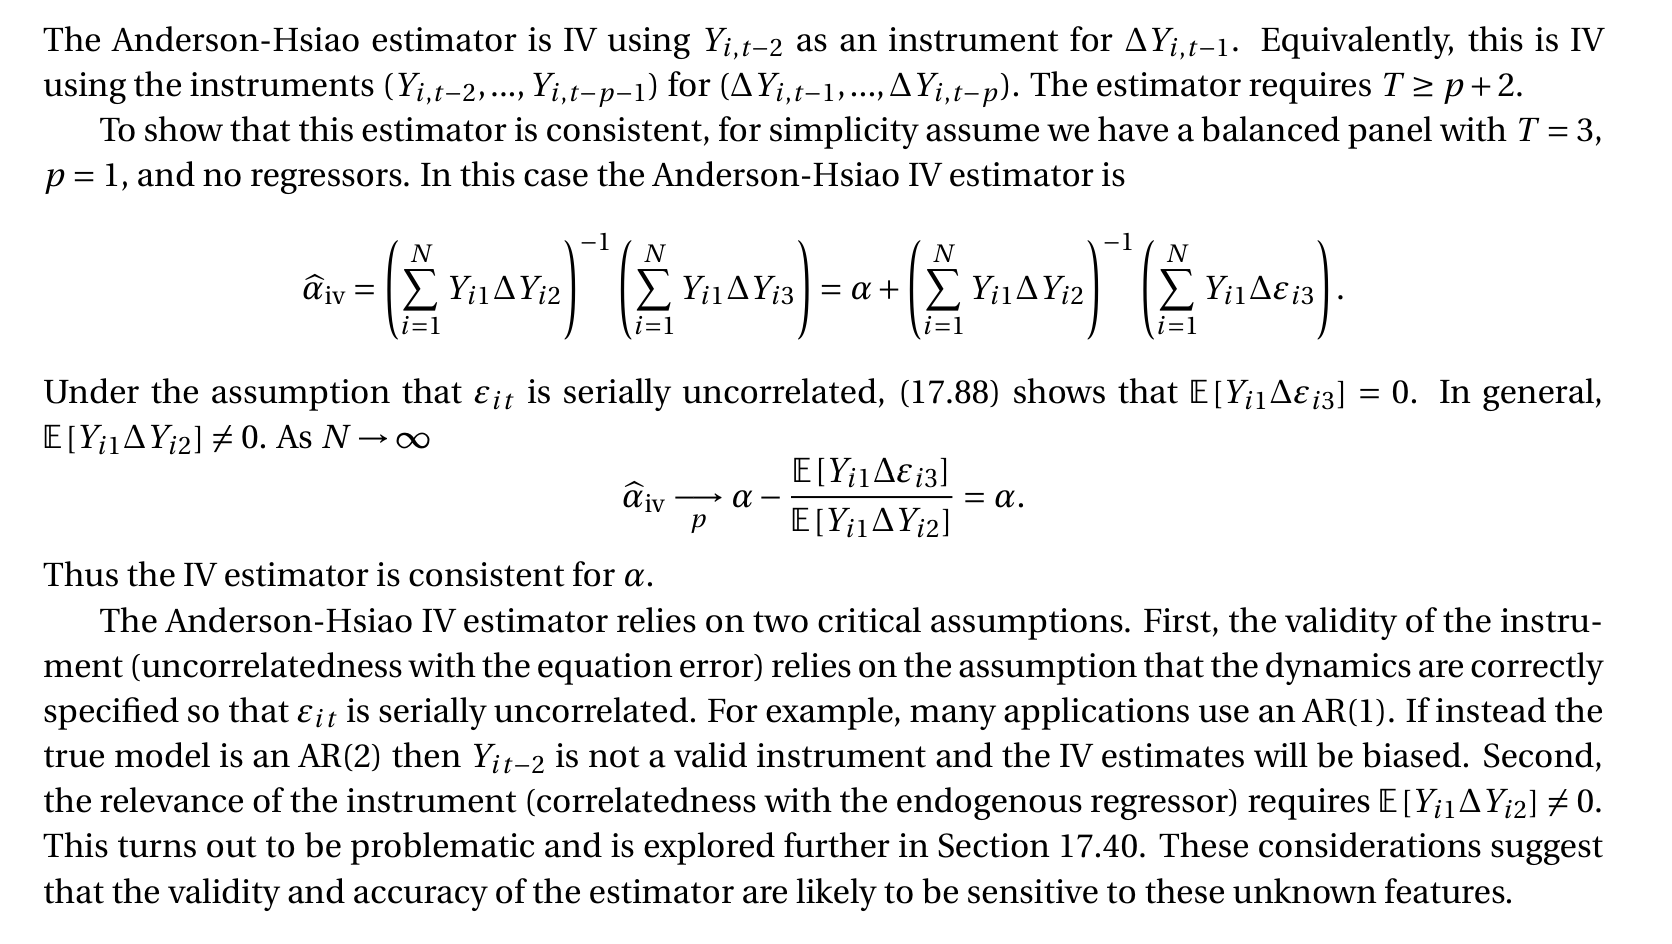
\includegraphics[width=\linewidth]{figures/Anderson-Hsiao-1981-2.png}
    \caption{Anderson and Hsiao(1981)}
\end{figure}

Using similar reasoning, other approaches use sequential exogeneity to circumvent FE methods 
altogether rather than to save their consistency. 
For example, Blundell and Bond (1998) start from the original specification:
\[y_{it} = x_{it}^{\prime} \beta + \alpha_i + u_{it}, \]
where correlation between $\alpha_{i}$ an $x_{it}$ is suspected to be due to $y_{i,t-1}$, contained in $x_{it}.$

\begin{definition}[Blundell and Bond(1998)]
    \begin{align*}
        y_{it} &= \alpha _i + \beta_1 y_{i,t-1} + u_{it} \\
        &= \beta_1 y_{i,t-1} + (u_{it} + \alpha_i) 
    \end{align*}
    Use $\Delta y_{i,t-1}$ as the IV for $y_{i,t-1}$
\end{definition}

% \chapter{Univariate Time Series}
% \section{Fundamentals of Time Series Analysis}
\label{sec:fundamentals-of-time-series-analysis}

A \textbf{time series} $Y_t \in \mathbb{R}^m$ is a process which is sequentially ordered over time.
The time series is univariate if $m = 1$ and multivariate if $m > 1$.

Most economic time series are recorded at discrete intervals such as annual, quarterly, monthly,
weekly, or daily. The number of observed periods $s$ per year is called the \textbf{frequency}.
In most cases we will denote the observed sample by the periods $t = 1, \cdots, n$. 

% Suppose we have a sample $\{w_i\}_{i=1}^n$, with $w_i = (y_i, x_i^{\prime})^{\prime}$, $\{w_{it}\}_{i=1:n, t=1:T}$.

% Now, we look at $\{w_t\}_{i=1}^T$, usually written as $y_t$, is univariate time series data.
Recall that cross-sectional observations are conventionally treated as random draws from an under-
lying population. This is not an appropriate model for time series processes due to serial dependence.
Instead, we treat the observed sample $\{y_1, \cdots, y_n\}$ as a realization of a dependent stochastic process. It is
often useful to view $\{y_1, \cdots, y_n\}$ as a subset of an underlying doubly-infinite sequence $\{\cdots, y_{t-1}, y_t, y_{t+1}, \cdots \}$.

A random vector $Y_t$ can be characterized by its distribution. A set such as $\{y_t, y_{t+1}, \cdots, y_{t+l} \}$ can be
characterized by its joint distribution. Important features of these distributions are their \textbf{means, vari-
ances, and covariances}.

\begin{remark}
    \

    Time series theory is a mixture of probabilistic and statistical concepts. 
    The probabilistic part is to study and characterize probability distributions 
    of sets of variables $y_t$ that will typically be dependent.
    The statistical problem is to determine the probability distribution of the time series
    given observations $y_1, \cdots, y_n$ at times $1,2, \cdots, n.$
    The resulting stochastic model can be used in two ways:
    \begin{itemize}
        \item understanding the stochastic system;
        \item predicting the ``future'', i.e. $y_{n+1}, y_{n+2}, \cdots$
    \end{itemize}
\end{remark}
% In the cross-sectional context, we average over $i$ to get 
% \[\mathbb{E}[y_i] = \int y_i f_y(y_i) d y_i.\]


As mentioned above, under time series data, we care about the joint distribution of random variable $y_t$.

We give the following definitions of the mean, variance, and covariance of a random variable $y_t$.
\begin{definition}[Mean function]\label{def:mean-function}
    \

    The mean function of a random variable $y_t$ is defined as
    \begin{gather*}
        \mu_t = \mathbb{E}[y_t] = \int y_t f_{t}(y_t) d y_t,
    \end{gather*}
    where $f_{t}(y_t)$ is the probability density function (PDF) of $y_t$.
\end{definition}

\begin{definition}[Autocovariance function]\label{def:autocovariance-function}
    \

    The autocovariance function of a random variable $y_t$ is defined as
    \begin{gather*}
        \gamma_{y}(r,s) = \operatorname{Cov}(y_r, y_s) = \mathbb{E}\Bigl[ (y_r - \mu_r)(y_s - \mu_s) \Bigr].
    \end{gather*}    
\end{definition}

\begin{definition}[Autocorrelation function]\label{def:autocorrelation-function}
    \

    The autocorrelation function (ACF) of a random variable $y_t$ is defined as
    \begin{gather*}
        \rho_{y}(r,s) = \frac{\operatorname{Cov}(y_r, y_s)}{\sqrt{\operatorname{Var}(y_r) \operatorname{Var}(y_s)}} = \frac{\gamma_{y}(r,s)}{\sqrt{\gamma_{y}(r,r) \gamma_{y}(s,s)}}.
    \end{gather*}
    
\end{definition}

\subsection{Stationarity and Strict Stationarity}

\begin{definition}[Stationarity]\label{def:weak-stationarity}
    \

    The time serie $\{y_t, t \in \mathbb{Z}\}$, is said to be stationary if:
    \begin{enumerate}
        \item[(i)] $\mathbb{E}[\vert y_t \vert ^2] < \infty$, for all $t$,
        \item[(ii)] $\mathbb{E}[y_t] = \mu $, for all $t$,
        \item[(iii)] $\gamma_y(r,s) = \gamma_y(r+t, s+t)$, for all $r,s,t \in \mathbb{Z}$. 
    \end{enumerate}
\end{definition}

\begin{remark}[About Stationarity]
    \
    
    Stationarity as just defined is frequently referred to in the literature as weak stationarity,
    covariance stationarity, stationarity in the wide sense or second-order stationarity.
    For us however the term stationarity, without further qualification, 
    will always refer to the properties specified by Definition \ref{def:weak-stationarity},
    that is, when we say stationary, we mean weak stationary.
\end{remark}

If $\{y_t, t \in \mathbb{Z}\}$ is \textbf{stationary}, then $\gamma_y(r,s) = \gamma_y(r-s, 0)$ for all $r,s \in \mathbb{Z}$.
It is therefore convenient to redefine the autocovariance function of a stationary
process as the function of just one variable,
\begin{gather*}
    \gamma_y(h) \equiv \gamma_y(h, 0) = \operatorname{Cov}(y_{t+h}, y_t), \quad \forall t, h \in \mathbb{Z}.
\end{gather*}
The function $\gamma_y(\cdot)$ will be referred to as the autocovariance function of $\{y_t\}$
and $\gamma_y(h)$ as its value at lag $h$. The autocorrelation function (ACF) of $\{y_t\}$
is defined analogously as the function whose value at lag $h$ is given by
\begin{gather*}
    \rho_y(h) = \frac{\gamma_y(t+h, t)}{\sqrt{\gamma_y(t+h, t) \gamma_y(t,t)} } = \frac{\gamma_y(h)}{\gamma_y(0)} = \operatorname{Corr}(y_{t+h}, y_t).
\end{gather*}
The auto-covariance and auto-correlation are functions $\gamma_y: \mathbb{Z} \to \mathbb{R}$ and $\rho_y: \mathbb{Z} \to [-1,1].$
Together with the mean $\mu = \mathbb{E}[y_t]$, they determine
the first and second moments of the stationary time series. 

% We also think of $y_t$ as a random variable (RV). Without the i.i.d. assumption,
% we generally have $T$ realizations of different and mutually dependent variables.
% \begin{gather*}
%     \mathbb{E}[y_t] = \int y_t f_{t}(y_t) d y_t = \mu_t, \\
%     \mathbb{V}[y_t] = \mathbb{E}\Bigl[(y_t - \mu_t)^2 \Bigr] = \gamma_{0,t}, \\
%     \operatorname{Cov}(y_t, y_{t-h}) = \mathbb{E}\Bigl[ (y_t - \mu_t)(y_{t-h} - \mu_{t-h}  ) \Bigr] = \gamma_{h,t}.
% \end{gather*}

% \begin{definition}[Weak Stationarity]\label{def:weak-stationarity}
%     \

%     $y_t$ is a weakly stationary process if
%     \begin{enumerate}
%         \item $\mu_t = \mu$ for all $t$,
%         \item $\gamma_{0,t} = \gamma_0$ for all $t$,
%         \item $\gamma_{h,t} = \gamma_h$ for all $t$.
%     \end{enumerate}
%     autocovariance function (ACF): $\{\gamma_0, \gamma_1, \cdots\}$
%     autocorrelation function: $\{\rho_0, \rho_1, \cdots \}$, where $\rho_h = \frac{\gamma_h}{\gamma_0}$.
% \end{definition}


\begin{definition}[Strict Stationarity]\label{def:strict-stationarity}
    \

    The time series $\{y_t, t \in \mathbb{Z}\}$ is said to be strictly stationary if the joint distribution of $(y_{t_1}, y_{t_2}, \cdots, y_{t_k})$
    and $(y_{t_1+h}, y_{t_2+h}, \cdots, y_{t_k+h})$ are the same for all $h$ and $k$ and $t_1, \cdots, t_k$.
\end{definition}
trict stationarity means intuitively that the graphs over two equal-length
time intervals of a realization of the time series should exhibit similar statistical
characteristics. For example, the proportion of ordinates not exceeding a
given level $x$ should be roughly the same for both intervals.

\subsection*{The Relation Between Stationarity and Strict Stationarity}

\begin{definition}[Ergodicity]\label{def:ergodicity}
    
    A process is said to be ergodic if time averages converge to ensemble averages.
    \begin{gather*}
        \lim_{n \to \infty} \vert \mathbb{E}[f(y_{t_1}, \cdots, y_{t_k}) g(y_{t_{1+n}}, \cdots, y_{t_{k+n}})] \vert - \vert \mathbb{E}[f(y_{t_1}, \cdots, y_{t_k})] \vert \vert \mathbb{E}[g(y_{t_1}, \cdots, y_{t_k})] \vert = 0, \\
        \forall t_1, \cdots, t_k, \text{ taking } k>l \text{w.l.o.g}.
    \end{gather*}
\end{definition}
% \section{ARMA Models}\label{sec:ARMA}
Classical regression is often insufficient for explaining all of the interesting dynamics
of a time series.
Instead, the introduction of correlation that may be generated through lagged linear relations
leads to proposing the \textbf{autoregressive (AR)} and \textbf{autoregressive moving average (ARMA)} models
that were presented in Whittle (1951) \cite{Whittle1951}.


\subsection{White Noise}\label{sec:whitenoise}

In many respects the simplest kind of time series $\{X_t\}$ is one in which
the random variables $X_t,t=0,\pm1,\pm2,\ldots$ are independently and identically distributed with zero mean and variance $\sigma^2.$
From a second order point of view i.e. ignoring all properties of the joint distributions of $\{X_t\}$
except those which can be deduced from the moments $\mathbb{E}[X_t]$ and $\mathbb{E}[X_s X_t]$,
such processes are identified with the class of all stationary processes having mean zero and \textit{autocovariance function}:
\begin{gather}\label{eq:WN}
    \gamma(h)=\Cov[X_t, X_{t+h}]=\begin{cases}
                                \sigma^2 & \mathrm{~if~}h=0,\\
                                0 & \mathrm{~if~}h\neq 0.
                            \end{cases}
\end{gather}

\begin{definition}[White Noise]\label{def:whitenoise}
    \
    
    The process $u_t$ is called \textbf{white noise}, written as
    \begin{gather*}
        u_t \sim WN(\mu, \sigma^2) 
    \end{gather*}
    if and only if $u_t$ has a mean of $\mu$ and covariance function \ref{eq:WN}.
    We call $u_t$ strong WN if $u_t \perp u_{t-h}, \forall t,h$ (i.e. $u_t$ and $u_{t-h}$ are independent).
\end{definition}

Usually, we deal with mean-zero WN: $u_t \sim WN(0, \sigma^2).$
\begin{note}
    \

    The distinction between (weak) WN and strong WN is only important for models where higher moments of $u_t$ matter, e.g.
    conditional heteroskedasticity models.
\end{note}
By this definition \ref{def:whitenoise}, we can easily know that any mean-zero i.i.d. sequence with finite variances (MDS) is a
white noise series. The converse is not true: there exist white noise series' that are not strictly stationary (MDS).

\textit{Therefore, the following types of shocks are nested: i.i.d., MDS, and white noise,
with i.i.d. being the most narrow class and white noise the broadest.}

If the WN process $u_t$ is Normal, then it is strong WN, as linear independence implies independence for Normal RVs.
We can simply write $u_t \overset{i.i.d.}{\sim} \mathcal{N}(0, \sigma^2)$.
Note that the Normal WN process is SS and ergodic as it consists of i.i.d. RVs at each $t$.

\begin{theorem}[Wold Decomposition]\label{thm:wolddecomp}
    \

    Suppose that $\{y_t\}$ is \textit{weak stationary}, with a finite variance (\textit{(we shall assume that it has mean zero, though this is not necessary)}).
    Then $y_t$ can be uniquely expressed as
    \begin{gather*}
        y_t = \sum_{j=0}^{\infty} \phi_j u_{t-j} + V_t 
    \end{gather*}
    where
    \begin{enumerate}
        \item $\{u_t\} \sim WN(0, \sigma^2)$;
        \item $\phi_0 = 1$ and $\sum_{j=0}^{\infty} \phi_j < \infty$;
        \item $\mathbb{E}[u_t V_s] = 0$ for all $t,s$;
        \item $V_t$ is deterministic.
    \end{enumerate}
\end{theorem}   

The Wold decomposition shows that $y_t$ can be written as a linear function of the white noise projection errors (\textbf{a linear process} that consists of (infinitely many) WN components) plus a deterministic process.
The Wold decomposition is a foundational result for linear time series analysis.
Since any covariance stationary process can be written in this format this justifies linear models as approximations.

The square summability condition $\sum_{j=0}^{\infty} \phi_j^2 < \infty$ ensures that the coefficients approach zero sufficiently quickly so that the impact of any $u_{t-j}$ on $y_t$ diminishes as $j$ increases.
We refer to $u_t$ as the innovation to the process $y_t$ at time $t$.

Note that the Wold decomposition does not restrict the distributional
family of $u_t$, nor does it exclude higher-order dependencies among $u_t$.

If $u_t$ is i.i.d, then $y_t$ is strictly stationary and ergodic as shown by our previous discussion of constituting ergodic process with definition \ref{def:ergodicity-plain}.

\subsection{ARMA\texorpdfstring{$(p,q)$}{(p,q)} Models}\label{sec:ARMApq}

A very wide class of stationary processes can be generated by using white
noise as the forcing terms in a set of linear difference equations. This leads to
the notion of an autoregressive-moving average (ARMA) process.

\begin{definition}[ARMA$(p,q)$ Process]\label{def:ARMApq}
    \
    
    The process $\{ y_t, t=0, \pm1, \pm2, \cdots\}$ is said to be an ARMA$(p,q)$ process if $y_t$ is stationary and for every $t$,
    \begin{gather}\label{eq:ARMApq}
        y_t - \phi_1 y_{t-1} - \cdots - \phi_p y_{t-p} = \alpha + \theta_1 u_{t-1} + \cdots + \theta_q u_{t-q} + u_t
    \end{gather}
    where $u_t \sim WN(0,\sigma^2)$, $\alpha = \mu \left( 1-\phi_1 - \cdots - \phi_p \right)$, $\mathbb{E}[y_t] = \mu$, and $\phi_p, \theta_q \neq 0.$
\end{definition}
The equation \ref{eq:ARMApq} can be written symbolically in the more compact form:
\begin{gather*}
    \phi (B) y_t = \alpha + \theta(B) u_t, t = 0, \pm1, \pm2, \cdots
\end{gather*}
where $\phi $ and $\theta$ are $p^{th}$ and $q^{th}$ order polynomials in the \textbf{backshift operator} $B$:
\begin{gather*}
    \phi (B) = 1 - \phi_1 B - \cdots - \phi_p B^p,\\
    \theta (B) = 1 + \theta_1 B + \cdots + \theta_q B^q
\end{gather*}
where $B$ is defined by:
\begin{gather*}
    B^j y_t = y_{t-j}, \quad j = 0, \pm1, \pm2, \cdots.
\end{gather*}
The polynomials $\phi(B)$ and $\theta(B)$ will be referred to as the \textbf{autoregressive} and \textbf{moving average} polynomials, respectively.

\subsection{Autoregressive Models}\label{sec:AR}

Autoregressive models are based on the idea that the current value of the series,
$y_t$, can be explained as a function of $p$ past values: $y_{t-1}, \cdots, y_{t-p},$
where $p$ determines the number of steps into the past needed to forecast the current value.

If $\theta(B) \equiv 0$ in ARMA$(p,q)$ \ref{eq:ARMApq}, then we have the \textbf{autoregressive} model of order $p$ (AR$(p)$):
\begin{definition}[AR$(p)$ Process]\label{def:ARp}
    \
    
    The process $\{ y_t, t=0, \pm1, \pm2, \cdots\}$ is said to be an AR$(p)$ process if $y_t$ is stationary and for every $t$,
    \begin{gather}\label{eq:ARp}
        y_t - \phi_1 y_{t-1} - \cdots - \phi_p y_{t-p} = \alpha + u_t
    \end{gather}
    where $u_t \sim WN(0,\sigma^2)$, $\alpha = \mu \left( 1-\phi_1 - \cdots - \phi_p \right)$, $\mathbb{E}[y_t] = \mu$, $\phi_p \neq 0.$
    This can be written symbolically in the more compact form:
    \begin{gather*}
        \phi (B) y_t = \alpha + u_t, t = 0, \pm1, \pm2, \cdots
    \end{gather*}
    where $\phi (B) = 1 - \phi_1 B - \cdots - \phi_p B^p$.
\end{definition}

\begin{eg}[AR(1) Process]\label{eg:AR1}
    \

    We initiate the investigation of AR models by considering the first-order model, AR(1), given by
    \begin{gather}\label{eq:AR1}
        y_t = \alpha + \phi_1 y_{t-1} + u_t, \quad u_t \sim WN(0, \sigma^2).
    \end{gather}
    Iterating backwards $k$ times, we get:
    \begin{align*}
        y_t &= \alpha + \phi y_{t-1} + u_t = \alpha + \phi \left( \alpha + \phi y_{t-2} + u_{t-1} \right) + u_t\\
        &= \alpha + \phi \alpha + \phi^2 y_{t-2} + \phi u_{t-1} + u_t\\
        &= \cdots \\
        &= \alpha \left( 1 + \phi + \phi^2 + \cdots + \phi^{k-1} \right) + \phi^k y_{t-k} + \sum_{j=0}^{k-1} \phi^j u_{t-j} \\
        &= \frac{\alpha}{1-\phi} + \phi^k y_{t-k} + \sum_{j=0}^{k-1} \phi^j u_{t-j}.
    \end{align*}
    This method suggests that, by continuing to iterate backward, and provided that $\vert \phi \vert < 1$,
    and $\mathbb{V}[y_t] < \infty$, we can represent an AR(1) model as a linear process given by
    \begin{gather}\label{eq:ARstationarysol}
        y_t = \frac{\alpha}{1-\phi} + \sum_{j=0}^{\infty} \phi^j u_{t-j}.
    \end{gather}
    Representation \ref{eq:ARstationarysol} is called the stationary solution of the model.
    In fact, by simple substitution,
    \begin{gather*}
        \underset{y_t}{\underbrace{\sum_{j=0}^{\infty} \phi^j u_{t-j}}} = \frac{\alpha}{1-\phi} +  \phi \underset{y_{t-1}}{\underbrace{\left(\sum_{k=0}^{\infty} \phi^k u_{t-k-1}\right)}} + u_t
    \end{gather*}
    The AR(1) process defined by \ref{eq:ARstationarysol} is stationary with mean
    \begin{gather*}
        \mathbb{E}[y_t] = \mathbb{E}\left[\frac{\alpha}{1-\phi}\right] + \sum_{j=0}^{\infty} \phi^j \mathbb{E}[u_{t-j}] = \frac{\alpha}{1-\phi}
    \end{gather*}
    and autocovariance function,
    \begin{align*}
        \gamma(h) &= \Cov[y_{t+h}, y_t] = \mathbb{E}\left[ \left( \sum_{j=0}^{\infty} \phi^j u_{t+h-j} \right) \left( \sum_{k=0}^{h} \phi^k u_{t-k} \right) \right] \\
        &= \mathbb{E}\left[ \left(u_{t+h} + \cdots + \phi^h u_t + \phi^{h+1} u_{t-1} + \cdots \right) \left( u_t + \phi u_{t-1} + \cdots \right) \right]\\
        &= \sigma^2 \sum_{j=0}^{\infty} \phi^{h+j} \phi^j \\
        &= \sigma^2 \phi^h \sum_{j=0}^{\infty} \phi^{2j} \\
        &= \frac{\sigma^2 \phi^h}{1-\phi^2}, \quad h \geq 0.
    \end{align*}
    Recall that $\gamma(h) = \gamma(-h)$, so we will only exhibit the autocovariance function for $h \geq 0.$
    We know it that the ACF of an AR(1) process is given by
    \begin{gather*}
        \rho(h) = \frac{\gamma(h)}{\gamma(0)} = \phi^h, \quad h \geq 0.
    \end{gather*}
    and $\rho(h)$ satisfies the recursion:
    \begin{gather*}
        \rho(h) = \phi \rho(h-1), \quad h \geq 1.
    \end{gather*}
\end{eg}

So, under $\vert \phi \vert < 1$, the AR(1) process is stable, since the effect of $u_{t-h}$ on $y_t$ dies out as $h \to \infty.$
If instead $\vert \phi \vert > 1$,then this effect diverges to infinity and we have an exploding process.
If $\phi = 1$, provided that $\alpha = 0$, $y_t$ is simply the sum of past innovations $u_t$:
$y_t = \sum_{h=0}^{\infty} u_{t-h}$. In that case, we call yt a unit-root or random walk process (with drift if $\alpha \neq 0$).
Under $\vert \phi \vert \geq 1$, the process is non-stationary and the ACF diverges to infinity.

\textcolor{red}{Extra material Needed}

\begin{eg}[AR(2) Process]\label{eg:AR2}
    \
    
    The AR(2) process is given by
    \begin{gather}\label{eq:AR2}
        y_t = \alpha + \phi_1 y_{t-1} + \phi_2 y_{t-2} + u_t, \quad u_t \sim WN(0, \sigma^2).
    \end{gather}
    This process can also be written as
    \begin{gather*}
        \phi(L) y_t = \alpha + u_t
    \end{gather*}
    where $\phi(L) = 1 - \phi_1 L - \phi_2 L^2$.
    Let $\frac{1}{\alpha_1}$ and $\frac{1}{\alpha_2}$ be the roots of $\phi(L) = 0$,
    we can rewrite the AR(2) model as:
    \begin{gather*}
        \alpha + u_t = (1-\alpha_1 L)(1-\alpha_2 L) y_t
    \end{gather*}
    We would like to find the conditions for the stationarity of $y_t$.
    It turns out that it's convenient to transform the AR(2) model \ref{eq:AR2} into a VAR(1) process.
    Set $\tilde{y}_t = (y_t, y_{t-1})^{\prime}$, which is stationary if and only if $y_t$ is stationary.
    Then equation \ref{eq:AR2} implies that:
    \begin{gather*}
        \begin{bmatrix}
            y_t \\
            y_{t-1}
        \end{bmatrix} = \begin{bmatrix}
            \alpha \\
            0
        \end{bmatrix} + \begin{bmatrix}
            \phi_1 & \phi_2 \\
            1 & 0
        \end{bmatrix} \begin{bmatrix}
            y_{t-1} \\
            y_{t-2}
        \end{bmatrix} + \begin{bmatrix}
            u_t \\
            0
        \end{bmatrix}
    \end{gather*}
    or, in matrix form:
    \begin{gather*}
        \tilde{y}_t = \mathbf{A} \tilde{y}_{t-1} + \tilde{u}_t
    \end{gather*}
    where $\mathbf{A} = \begin{bmatrix}
        \phi_1 & \phi_2 \\
        1 & 0
    \end{bmatrix}$ and $\tilde{u}_t = \begin{bmatrix}
        \alpha + u_t \\
        0
    \end{bmatrix}$.
\end{eg}

% \section{Inference of Univariate Time Series Models}
\label{sec:inference-univariate-time-series-models}

\begin{gather*}
    y_t \sim \text{WS} \Leftrightarrow y_t \sim I(0) \\
    \Delta y_t \sim \text{WS} \Leftrightarrow y_t \sim I(1) \\
    \underset{\Delta^2 y_t}{\underbrace{\Delta y_t - \Delta y_{t-1}}} \sim \text{WS} \Leftrightarrow y_t \sim I(2)
\end{gather*}

\subsection{Estimation of AR(p) Models}

\begin{eg}
    \

    Let's consider the following AR(1) model:
    \begin{gather*}
        y_t = \alpha + \beta y_{t-1} + u_t = x_t^{\prime} \phi + u_t\\
        x_t = \begin{bmatrix} 1 \\ y_{t-1} \end{bmatrix}, \phi = \begin{bmatrix} \phi_0 \\ \phi_1 \end{bmatrix} \\
        \quad \text{where } u_t \text{ is a white noise process}
    \end{gather*}
    As $u_t$ is the white noise, $\mathbb{E}[x_t u_t] = 0$, and that $x_t$ is a function of $u_{t-1}, u_{t-2}, \cdots$.
    If $u_t$ is strict white noise, e.g. $u_t \sim i.i.d. \mathcal{N}(0, \sigma^2)$, then $\mathbb{E}[u_t | x_t] = \mathbb{E}[u_t] = 0$.
\end{eg}

% \subsubsection{OLS estimator}

We consider estimation of an AR(p) model for stationary, ergodic, and non-deterministic $y_t$.
The model is where $x_t = [1, y_{t-1}, \cdots, y_{t-p}]^{\prime} $, $\phi = [\phi_0, \phi_1, \cdots, \phi_p]^{\prime} $
and $u_t \sim WN(0, \sigma^2)$.

\subsubsection{OLS estimator}\label{AR-OLS}

The OLS estimator is given by:
\begin{gather*}
    \hat{\phi} = \argmin_{\phi} \sum_{t=1}^{T} u_t^2 \\
    U^{\prime} U = (Y - X\phi)^{\prime} (Y - X\phi) \\
    \Rightarrow \hat{\phi} = (X^{\prime} X)^{-1} X^{\prime} Y = \left( \sum_{t=1}^{n} x_t x_t^{\prime} \right)^{-1} \left( \sum_{t=1}^{n} x_t y_t \right).
\end{gather*}
This notation presumes that there are $n+p$ total observations on $y_t$ from which the first $p$ are used as initial conditions so that
$x_1 = \left( 1, y_0, y_{-1}, \cdots, y_{p+1} \right)$ is defined.

\subsubsection{Consistency of OLS Estimator}\label{sec:consistency-AR-OLS}

The OLS residuals are $\hat{u}_t = y_t - x_t^{\prime} \hat{\phi}$.
The error variaance can be estimated by $\hat{\sigma}^2 = \frac{1}{n} \sum_{t=1}^{n} \hat{u}_t^2$
or $s^2 = \frac{1}{n-p-1} \sum_{t=1}^{n} \hat{u}_t^2.$
Fot the true model, if $y_t$ is strictly stationary (SS), and ergodic (E), then so are $x_t x_t^{\prime} $ and $x_t y_t$.
They have finite means $\mathbb{E}[y_t^2] < \infty.$
Under these assumptions the Ergodic Theorem implies that
\begin{gather*}
    \frac{1}{n} \sum_{t=1}^{n} x_t x_t^{\prime} \overset{p}{\rightarrow} \mathbb{E}[x_t x_t^{\prime}] = Q \\
    \frac{1}{n} \sum_{t=1}^{n} x_t y_t \overset{p}{\rightarrow} \mathbb{E}[x_t y_t]
\end{gather*}
and we know that OLS is consistent for $\phi$ if $x_t$ is uncorrelated with $u_t$.
\begin{align*}
    \hat{\phi} &= (X^{\prime} X)^{-1} X^{\prime} Y \\
    &= (X^{\prime} X)^{-1} X^{\prime} (X\phi + U) \\
    &= \phi + (X^{\prime} X)^{-1} X^{\prime} U \\
    &= \phi + \left( \frac{1}{T} \sum_{t} x_t x_t^{\prime} \right)^{-1} \frac{1}{T} \sum_{t=1}^{T} x_t u_t \\
    & \overset{p}{\rightarrow} \phi + \mathbb{E}[x_t x_t^{\prime}] \mathbb{E}[x_t u_t] \\
    &= \phi
\end{align*}
It is straightforward to show that $\hat{\sigma}^2$ is consistent as well.
\begin{theorem}[AR(p) OLS Consistency]
    \

    If $y_t$ is strictly stationary, ergodic, not purely deterministic, and $\mathbb{E}[y_t^2] < \infty$,
    then the OLS estimator $\hat{\phi}$ is consistent for $\phi$, and $\hat{\sigma}^2 \overset{p}{\rightarrow} \sigma^2$ as $n \to \infty.$
\end{theorem}

\begin{note}
    \

    This shows that under very mild conditions the coefficients of an AR(p) model can be consistently estimated by least squares.
    Once again, this does not require that the series $y_t$ is actually an AR(p) process.
    It holds for any stationary process with the coefficient defined by projection.
\end{note}
% So, $\hat{\phi}$ is consistent.

\subsubsection{Asymptotic Normality of OLS Estimator}\label{sec:asymptotic-AR-OLS}

The asymptotic distribution of the least squares estimator $\hat{\phi}$ depends on the stochastic assumptions.
Specifically, we assume that the error $u_t$ is a MDS (definition \ref{def:martingale-difference-sequence}).
An important implication is taht since $x_t = \left( 1, y_{t-1}, \cdots, y_{t-p} \right)^{\prime} $ is part of the information set $\mathcal{F}_{t-1}$, by the conditioning theorem,
\begin{gather*}
    \mathbb{E}[x_t u_t | \mathcal{F}_{t-1}] = x_t \mathbb{E}[u_t | \mathcal{F}_{t-1}] = 0.
\end{gather*}
Thus $x_t u_t$ is a MDS. It has a finite variance if $u_t$ jas a finite fourth moment.
We know that $y_t$ can be written in MA$(\infty)$ form:
\begin{gather*}
    y_t = \mu + \sum_{j=0}^{\infty} \phi_j u_{t-j} 
\end{gather*}
with $\sum_{j=0}^{\infty} \vert \phi_j \vert < \infty$.
Using Minkowski's Inequality,
\begin{gather*}
    \left( \mathbb{E} \vert y_t \vert^4 \right)^\frac{1}{4} \leq \sum_{j=0}^{\infty} \vert \phi_j \vert \left( \mathbb{E} \vert u_{t-j} \vert^4 \right)^\frac{1}{4} < \infty.
\end{gather*}
Thus $\mathbb{E}[y_t^4] < \infty $. The Cauchy-Schwarz inequality then shows that $\mathbb{E} \lVert x_t u_t \rVert^2 < \infty.$
We can then apply the MDS CLT \ref{thm:mds-clt} to show that:
\begin{gather*}
    \frac{1}{\sqrt{n}} \sum_{t=1}^{n} x_t u_t \overset{d}{\rightarrow} \mathcal{N}(0, \Sigma)
\end{gather*}
where $\Sigma = \mathbb{E}[x_t x_t^{\prime} u_t^2].$
\begin{theorem}[MDS AR(p) Asymptotic Normality]\label{thm:mds-ar-asymptotic-normality}
    \
    
    If $y_t$ follows the $AR(p)$ model, all roots of $\phi(z)$ lie outside the unit circle,
    (all eigenvalues have absolute value smaller than 1), $\mathbb{E}[u_t | \mathcal{F}_{t-1}] = 0$, $\mathbb{E}[u_t^4] < \infty$,
    and $\mathbb{E}[u_t^2] > 0$, then as $n \to \infty$, the OLS estimator $\hat{\phi}$ is asymptotically normal:
    \begin{gather*}
        \sqrt{n}\left( \hat{\phi} - \phi \right) \overset{d}{\rightarrow} \mathcal{N}(0, V)
    \end{gather*}
    where $V = Q^{-1} \Sigma Q^{-1}.$ ($Q = \mathbb{E}[x_t x_t^{\prime}].$)
\end{theorem}
This is identical in form to the asymptotic distribution of least squares in cross-section regression.
The implication is that asymptotic inference is the same. In particular, the asymptotic covariance matrix
is estimated just as in the cross-section case.
\begin{theorem}[MDS AR(p) Asymptotic Normality(continue)]\label{thm:mds-ar-asymptotic-normality-2}
    \
    
    If we further assume that $\mathbb{E}[u_t^2 | \mathcal{F}_{t-1}] = \sigma^2$, then as $n \to \infty$,
    \begin{gather*}
        \sqrt{n}\left( \hat{\phi} - \phi \right) \overset{d}{\rightarrow} \mathcal{N}(0, V)
    \end{gather*}
    where $V = \sigma^2 Q^{-1}.$   
\end{theorem}
These results show that under correct specification (a MDS error) the format of the asymptotic distribution of the least squares estimator exactly parallels the cross-section case.

If the $AR(p)$ model holds WN errors, as we originally assumed ($u_t \sim WN(0, \sigma^2)$), the MDS CLT doesn't hold\footnote{As we have previously shown under the definition \ref{def:whitenoise}, there exist white noises that are not strictly stationary, hence not MDS.}.
Instead, if $y_t$ is strong mixing, we can use the central limit theorem for mixing proceses.
\begin{theorem}[Mixing AR Asymptotic Normality]\label{thm:mixing-ar-asymptotic-normality}
    \
    
    Assume $y_t$ is strictly stationary, ergodic, and for some $r>4$, $\mathbb{E}\vert y_t \vert^r < \infty$
    and the mixing coefficients $\sum_{l=1}^{\infty} \phi(l)^{1-\frac{r}{4}} < \infty$.
    Let $\phi $ be defined as the best linear projection coefficients, $\phi = \left(\mathbb{E}[x_t x_t^{\prime} ]\right)^{-1} \mathbb{E}[x_t y_t]$
    from an AR(p) model, with projection errors $u_t$. Let $\hat{\phi}$ be the OLS estimator of $\phi$.
    \begin{gather*}
        \Omega = \sum_{l=-\infty}^{\infty} \mathbb{E} \left[ x_{t-l} x_t^{\prime} u_t u_{t-l} \right]
    \end{gather*}
    is convergent and
    \begin{gather*}
        \sqrt{n} (\hat{\phi} - \phi) \overset{d}{\rightarrow} \mathcal{N}(0, V)
    \end{gather*}
    where $V = Q^{-1} \Omega Q^{-1}.$
\end{theorem}

To simplify our case, we can assume that our model is with strict WN $u_t \sim \mathcal{N}(0, \sigma^2)$.
We can thus have the following result using theorem \ref{thm:mixing-ar-asymptotic-normality}:
\begin{align*}
    \sqrt{T}(\hat{\phi} - \phi) &= \sqrt{T} \left( \frac{1}{T} \sum_{t=1}^{T} x_t u_t \right)^{\prime} \left( \frac{1}{T} \sum_{t=1}^{T} x_t x_t^{\prime} \right)^{-1} \\
    & \overset{d}{\rightarrow} \mathbb{E}[x_t x_t^{\prime}]^{-1} \mathcal{N} \left(0, \mathbb{V}\left[\frac{1}{\sqrt{T}} \sum_{t} x_t u_t \right]\right)
\end{align*}
where
\begin{align*}
    \frac{1}{T} \mathbb{V}\left[\sum_{t=1}^{T} x_t u_t\right] &= \frac{1}{T} \sum_{t} \mathbb{V}[x_t u_t] + \frac{1}{T} \sum_{t} \sum_{\tau \neq t} \operatorname{Cov}(x_t u_t, x_\tau u_\tau) \\
    &= \mathbb{E}[u_{t}^2 x_t x_t^{\prime}] + \frac{1}{T} \sum_{t} \sum_{\tau \neq t} \mathbb{E}[u_t u_{\tau}] x_t x_{\tau}^{\prime} \\
    \text{Assume that } u_t \sim \mathcal{N}(0, \sigma^2)
    &= \mathbb{E}[u_t^2] \mathbb{E}[x_t x_t^{\prime}] + \frac{1}{T} \sum_{t} \sum_{\tau} \mathbb{E}[u_t] \mathbb{E}[u_{\tau}] \mathbb{E}[x_t x_{\tau}^{\prime}] \\
    &= \sigma^2 \mathbb{E}[x_t x_t^{\prime}] \\
    \Rightarrow \sqrt{T}(\hat{\phi} - \phi) &\overset{d}{\rightarrow} \mathcal{N} \left(0, Q^{-1} \sigma^2 Q Q^{-1} \right) = \mathcal{N}\left(0, \underset{V}{\underbrace{\sigma^2 \mathbb{E}[x_t x_t^{\prime}]^{-1}}} \right)
\end{align*}
For the estimators:
\begin{gather*}
    \hat{V} = \hat{\sigma}^2 \left( \frac{1}{T} \sum_{t=1}^{T} x_t x_t^{\prime} \right)^{-1} \\
    \hat{\sigma}^2 = \frac{1}{T} \sum_{t=1}^{T} \hat{u}_t^2
\end{gather*}
like with cross sectional data.

Unlike the cross-sectional case, $x_t$ consists of lagged values of $y_t$,
we can also use the moments implied by our supposed model to estimate $\mathbb{E}[x_t x_t^{\prime}].$
In addition, if we consider $AR(1)$ model, where we have $x_t = [1, y_{t-1}]^{\prime}$:
\begin{gather*}
    \mathbb{E}[x_t x_t^{\prime}] = \mathbb{E}\left[ \begin{bmatrix}
        1 \\
        y_{t-1}
    \end{bmatrix} \begin{bmatrix}
        1 & y_{t-1} 
    \end{bmatrix} \right] = \mathbb{E} \begin{bmatrix}
        1 & y_{t-1} \\
        y_{t-1} & y_{t-1}^2
    \end{bmatrix} = \begin{bmatrix}
        1 & \frac{\phi_0}{1 - \phi_1} \\
        \frac{\phi_0}{1 - \phi_1} & \mathbb{E}[y_t^2]
    \end{bmatrix} \\
    \text{where } \mathbb{E}[y_t] = \frac{\phi_0}{1 - \phi_1} , \mathbb{V}[y_t] = \frac{\sigma^2}{1 - \phi_1^2}, \mathbb{E}[y_t^2] = \mathbb{V}[y_t] + \mathbb{E}[y_t]^2 = \frac{\sigma^2}{1 - \phi_1^2} + \frac{\phi_0^2}{(1 - \phi_1)^2}
\end{gather*}
For the estimator, 
\begin{gather*}
    \hat{\mathbb{E}}[x_t x_t^{\prime}] = \begin{bmatrix}
        1 & \frac{\hat{\phi}_0^2}{1 - \hat{\phi}_1} \\
        \frac{\hat{\phi}_0^2}{1 - \hat{\phi}_1} & \frac{\hat{\sigma}^2}{1 - \hat{\phi}_1^2} + \frac{\hat{\phi}_0^2}{(1 - \hat{\phi}_1)^2}
    \end{bmatrix}
\end{gather*}

\subsubsection{MLE estimator}
\begin{align*}
    \hat{\phi}_{ML} &= \argmax_{\phi} p\left( y_T | y_1, \cdots, y_{T-1}, \phi \right) p\left( y_{T-1}, y_{T-2}, \cdots, y_1 | \phi, y_0 \right) \\
    &= \prod_{t=1}^{T} p(y_t | y_{1:t-1}, \phi)
\end{align*}
Under $AR(1)$, only the first lag is important for the distribution of $y_t$.
\begin{gather*}
    p(y_t | y_{1:t-1}, \phi) = p(y_t | \phi, y_{t-1})
\end{gather*}
We further assume $u_t \sim \mathcal{N} (0, \sigma^2)$, then we get: $y_t | y_{t-1} \sim \mathcal{N} (\phi y_{t-1}, \sigma^2)$, thus
\begin{align*}
    p(y_{1:T} | \phi, y_0) &= \prod_{t=1}^{T}(2 \pi \sigma^2)^{-1/2} \exp\left\{-\frac{1}{2 \sigma^2} (y_t - \phi y_{t-1})^2\right\} \\
    &= (2 \pi \sigma^2)^{-T/2} \exp\left\{-\frac{1}{2 \sigma^2} \sum_{t=1}^{T} (y_t - \phi y_{t-1})^2\right\} \\
    &= (2 \pi \sigma^2)^{-T/2} \exp\left\{-\frac{1}{2 \sigma^2} (Y - X \phi)^{\prime} (Y - X \phi) \right\}
\end{align*}

\subsubsection{Unit-Root}

Consider the $AR(1)$ process under the presence of a unit-root:
\begin{gather*}
    y_t = \phi_0 + \phi_1 y_{t-1} + u_t, \quad \phi_1 = 1
\end{gather*}
In this case, the process is not WS, thus not Strictly stationary and Ergodic.

If $\phi_0 = 0$, then 
\begin{gather*}
    % \hat{\phi}_1 = \frac{\mathbb{E}[V_{t-2} y_t]}{\mathbb{E}[y_{t-1}^2]} \\
    \sqrt{T}(\hat{\phi}_1 - \phi_1) \overset{d}{\rightarrow} \mathcal{N}\left(0, \frac{\sigma^2}{\mathbb{V}[y_t]}\right) 
\end{gather*}
If we further assume that $y_0=0$, the process $y_t$ can be represented as 
\begin{gather*}
    y_t = \sum_{\tau=1}^{t} u_{\tau}
\end{gather*}
The central limit theorem for i.i.d. random variables implies that:
\begin{gather*}
    \frac{y_T}{\sqrt{T}} = \frac{1}{\sqrt{T}} \sum_{\tau=1}^{T} u_{\tau} \overset{d}{\rightarrow} \mathcal{N}(0, \sigma^2)
\end{gather*}
which suggests that 
\begin{gather*}
    \frac{1}{T} \sum_{t=1}^{T} y_t = \frac{1}{\sqrt{T}} \sum_{t=1}^{T}\left[ \sqrt{\frac{t}{T}} \frac{1}{\sqrt{t}} \sum_{\tau =1}^{t} u_{\tau} \right]
\end{gather*}
will not converge to a constant in probability but instead to a random variable.

Thus, we have a special distribution derived by Dickey and Fuller:
\begin{gather*}
    T(\hat{\phi}_1 - \phi_1) \overset{d}{\rightarrow}  \text{ Dickey-Fuller distribution}
\end{gather*}

\subsection{Estimating Regressions with Autocorrelated Errors}
Suppose we want to estimate $y_t = x_t^{\prime} \beta + u_t$,
where $x_t$ contains $k$ variables measuredover time (and potentially a constant).
In such time series, the error $u_t$ is likely autocorrelated, $\mathbb{E}[u_t u_{\tau} ] \neq 0$ for $t \neq \tau$.
This leads to different standard errors for the OLS estimator $\hat{\beta}$ under the i.i.d. (cross-sectional) case.

Assumiong that $\mathbb{E}[x_t u_t] = 0$, and that both $u_t$ and $x_t$ are strictly stationary and ergodic,
we can apply the LLN for such processes.
\begin{align*}
    \hat{\beta} &= (X^{\prime} X)^{-1} X^{\prime} Y \\
    &= (X^{\prime} X)^{-1} X^{\prime} (X \beta + U) \\
    &= \beta + (X^{\prime} X)^{-1} X^{\prime} U \\
    &= \beta + \left( \frac{1}{T} \sum_{t=1}^{T} x_t x_t^{\prime} \right)^{-1} \frac{1}{T} \sum_{t=1}^{T} x_t u_t \\
    & \rightarrow \beta + \mathbb{E}[x_t x_t^{\prime}]^{-1} \mathbb{E}[x_t u_t] \\
    &= \beta \text{ for SS+E, TS}
\end{align*}
and that
\begin{align*}
    \sqrt{T}(\hat{\beta} - \beta) &= \sqrt{T} \left( \frac{1}{T} \sum_{t=1}^{T} x_t u_t \right)^{\prime} \left( \frac{1}{T} \sum_{t=1}^{T} x_t x_t^{\prime} \right)^{-1} \\
    &\overset{d}{\rightarrow} \mathcal{N}\left(0, V\right)
\end{align*}
where
\[
V = \mathbb{E}[x_t x_t^{\prime}]^{-1} \mathbb{V}\left[\frac{1}{\sqrt{T}} \sum_{t=1}^{T} x_t u_t\right] \mathbb{E}[x_t x_t^{\prime}]^{-1}.
\]
The term in the middle can be written as:
\begin{align*}
    \mathbb{V}\left[\frac{1}{\sqrt{T}} \sum_{t=1}^{T} x_t u_t\right] &= \frac{1}{T} \sum_{t=1}^{T} \mathbb{V}\left[x_t u_t\right] + \frac{1}{T} \sum_{t=1}^{T} \sum_{\tau \neq t} \Cov[x_t u_t ,x_{\tau} u_{\tau}] \\
    &= \frac{1}{T} \sum_{t=1}^{T} \mathbb{E}[u_t^2 x_t x_t^{\prime}] + \frac{1}{T} \sum_{t} \sum_{\tau \neq t} \mathbb{E}[x_t x_{\tau}^{\prime} u_t u_{\tau}] \\
    &= \mathbb{E}[x_t x_t^{\prime} u_t^2] + \sum_{h=1}^{T-1} \mathbb{E}\left[u_t u_{t-h} \left(x_t x_{t-h}^{\prime} + x_{t-h} x_t^{\prime} \right)\right].
\end{align*}
\begin{enumerate}
    \item $x_t u_t$ is not autocorrelated, then the second term is zero.
        \begin{enumerate}
            \item[(a)] if $\mathbb{E}[u_t^2] = \sigma^2$ (homoskedasticity), then $\mathbb{E}[u_t^2 x_t x_t^{\prime}] = \sigma^2 \mathbb{E}[x_t x_t^{\prime}]$,
            the same expression as obtained under a homoskedastic linear regression model for cross-sectional data.
            \item[(b)] if $\mathbb{E}[u_t^2] = f(x_t)$ (heteroskedasticity), the first term does not simplify,
            and we construct the heteroskedasticity-robust variance $\mathbb{E}[x_t x_t^{\prime}]^{-1} \mathbb{E}[x_t x_t^{\prime} u_t^2] \mathbb{E}[x_t x_t^{\prime}]^{-1}$.
            We just eimate it by replacing the expectation operators with time averages and $\hat{u}_t$: $\frac{1}{T} \sum_{t} \hat{u}_t^2 x_t x_t^{\prime}.$
        \end{enumerate}
    \item $x_t u_t$ is autocorrelated, then we can write $V$ as:
        \begin{gather*}
            \mathbb{E}[u_t^2 x_t x_t^{\prime}] + \frac{1}{T} \sum_{t} \sum_{h=1}^{T-1} \mathbb{E}[u_t u_{t-h} x_t x_{t-h}] \\
            = \frac{1}{T} \sum_{t} \hat{u}_t^2 x_t x_t^{\prime} + \frac{1}{T} \sum_{t} \sum_{h=1}^{T-1} 2 \hat{u}_t \hat{u}_{t-h} x_t x_{t-h}  
        \end{gather*}
\end{enumerate}

\begin{remark}
    \

    For the second case, we recall the original version of variance:
    \begin{gather*}
        \mathbb{V}\left[\frac{1}{T} \sum_{t=1}^{T} x_t u_t\right] = \frac{1}{T} \sum_{t=1}^{T} \sum_{\tau=1}^{T} \Cov[u_t, u_{\tau}] x_t x_{\tau}^{\prime}  
    \end{gather*}
    We assume that $\vert \Cov[u_t, u_{\tau}] \vert \leq \vert t-\tau \vert^{\kappa} $ where $\kappa>1$.
    Since $u_t u_{\tau}$ can be treated as a ``preestimator'' of $\Cov[u_t, u_{\tau}]$,
    we can replace the covariance with $u_t u_{\tau}$ and weight it with $\lambda(t-\tau)$ to yield the Newey-West/HAC estimator:
    \begin{gather*}
        \hat{\sigma}^2 = \frac{1}{T} \sum_{t=1}^{T} \sum_{\tau=1}^{T} \lambda_m(t-\tau) u_t u_{\tau} x_t x_{\tau}^{\prime}.
    \end{gather*}
\end{remark}

% \chapter{Multivariate Time Series}
% Multi GLP:
\begin{gather*}
    y_t = B(L) u_t = \sum_{l=0}^{\infty} B_l u_{t-l}, \quad u_t \sim WN(0, \Sigma)
\end{gather*}
where $B_0 = I$ and $\sum_{l=0}^{\infty} \lVert B_l \rVert^2 < \infty.$

\section{Vector Autoregressions (VARs)}\label{sec:var}

As in the previous lecture, we have built a VAR(1) model for solving the AR(2) process.
\begin{gather*}
    y_t = \Phi_0 + \Phi_1 y_{t-1} + u_t, \quad u_t \sim WN(0, \Sigma)
\end{gather*}
e.g. $n=2$:
\begin{gather*}
    \begin{bmatrix}
        y_{1t} \\
        y_{2t}
    \end{bmatrix} = \begin{bmatrix}
         \Phi_{0,1} \\
         \Phi_{0,2} \\
    \end{bmatrix} + \begin{bmatrix}
        \Phi_{1,11} & \Phi_{1,12}  \\
        \Phi_{1,21} & \Phi_{1,22}  \\
    \end{bmatrix}
    \begin{bmatrix}
        y_{1,t-1} \\
        y_{2,t-1}
    \end{bmatrix} + \begin{bmatrix}
         u_{1t} \\
         u_{2t} \\
    \end{bmatrix}, \quad u_t \sim WN(0, \Sigma)
\end{gather*}
where $u_t \sim  WN\left( \begin{bmatrix}
     0 \\
     0 \\
\end{bmatrix}, \begin{bmatrix}
    \sigma_{11} & \sigma_{12} \\
    \sigma_{21} & \sigma_{22} \\
\end{bmatrix} \right)$.

\begin{definition}[VAR$(p)$]
    \

    A VAR(p) model is a system of $n$ equations of the form:
    \begin{gather*}
        y_t = \Phi_0 + \sum_{i=1}^{p} \Phi_i y_{t-i} + u_t, \quad u_t \sim WN(0, \Sigma)
    \end{gather*}
    where $y_t$ is an $n$-dimensional vector, $\Phi_0$ is an $n$-dimensional vector of constants, $\Phi_i$ are $n \times n$ matrices of coefficients, and $u_t$ is an $n$-dimensional vector of white noise errors.
\end{definition}

\subsection{Stationarity of VAR$(p)$}\label{sec:stationarity-var}
\begin{eg}
    \

    Consider the VAR(2) model:
    \begin{gather*}
        y_t = \Phi_0 + \Phi_1 y_{t-1} + \Phi_2 y_{t-2} + u_t
    \end{gather*}
    or we write in companion form:
    \begin{gather*}
        \begin{bmatrix}
            y_t \\
            y_{t-1}
        \end{bmatrix} = \begin{bmatrix}
            \Phi_0 \\
            0
        \end{bmatrix} + \begin{bmatrix}
            \Phi_1 & \Phi_2 \\
            I & 0
        \end{bmatrix} 
        \begin{bmatrix}
            y_{t-1} \\
            y_{t-2}
        \end{bmatrix} + \begin{bmatrix}
             u_t \\
             0 \\
        \end{bmatrix}
    \end{gather*}
    we can simply write:
    \begin{gather*}
        X_t = F_0 + F_1 X_{t-1} + v_t
    \end{gather*}
    We take mean on both sides,
    \begin{gather*}
        \mathbb{E}[y_t] = \Phi_0 + \Phi_1 \mathbb{E}[y_{t-1}] + \Phi_2 \mathbb{E}[y_{t-2}] + 0
    \end{gather*}
    as $\mathbb{E}[y_t] = \mathbb{E}[y_{t-1}] = \mathbb{E}[y_{t-2}] = \mu$,
    we know that $\mu = \left(1 - \Phi_1 - \Phi_2\right)^{-1} \Phi_0.$
\end{eg}

\subsection{Moments \& GLP-Representation}
Consider first for a VAR(1). Repeatedly inserting for lags $y_{t-1}$, we get:
\begin{align*}
    y_t &= \Phi_0 + \Phi_1 y_{t-1} + u_t \\
    &= \Phi_0 + \Phi_1 (\Phi_0 + \Phi_1 y_{t-2} + u_{t-1}) + u_t \\
    &= \Phi_0 + \Phi_1 \Phi_0 + \Phi_1^2 y_{t-2} + \Phi_1 u_{t-1} + u_t \\
    &= \cdots \\
    &= \sum_{l=0}^{\infty} \Phi_1^l \Phi_0 + \sum_{l=0}^{\infty} \Phi_1^l u_{t-l} + \lim_{k \to \infty} \Phi_1^k y_{t-k} \\
    &= \frac{\Phi_0}{1 - \Phi_1} + \sum_{l=0}^{\infty} \Phi_1^l u_{t-l}
\end{align*}
if $\Phi_1$ jas all eigenvalues in the unit circle, then $\lim_{k \to \infty} \Phi_1^k y_{t-k} = 0$.
Based on this expresison, we can get the ACF:
\begin{align*}
    \Gamma_h = \Cov[y_t, y_{t-h}] &= \mathbb{E}\left[ \left(\sum_{t=0}^{\infty}\Phi_1^l u_{t-l} \right) \left( \sum_{k=0}^{\infty}\Phi_1^k u_{t-h-k} \right)^{\prime} \right] \\
    &= \sum_{k=0}^{\infty} \mathbb{E}\left[ \left(\Phi_1^k u_{t-h-k} \right) \left(\Phi_1^k u_{t-h-k} \right)^{\prime} \right] \\
    &= \sum_{k=0}^{\infty} \Phi_1^{h+k}  \mathbb{E}\left[ u_{t-h-k} u_{t-h-k}^{\prime} \right] \Phi_1^{k^{\prime}} \\
    &= \sum_{k=0}^{\infty} \Phi_1^{h+k} \Sigma \Phi_1^{k^{\prime}}
\end{align*}
As we generalize this to VAR(p) ($X_t = F_0 + F_1 X_{t-1} + v_t$), we can get:
\begin{gather*}
    \Gamma_h^X = \sum_{k=0}^{\infty} F_1^{h+k} \Sigma^v F_1^{k^{\prime}}
\end{gather*}
where $\mathbb{V}[u_t] = \Sigma^v = \begin{bmatrix}
    \Sigma^v & 0 \\
    0 & 0 \\
\end{bmatrix}$.
And we can have the ACF for the original $y_t$:
\begin{align*}
    \Gamma_h^y = \Cov[y_t, y_{t-h}] &= \Cov[MX_t, MX_{t-h}] \\
    &= M \Cov[X_t, X_{t-h}] M^{\prime} \\
    &= \sum_{k=0}^{\infty} M F_1^{h+k} \Sigma^v F_1^{k^{\prime}} M^{\prime} \\
    &= \sum_{k=0}^{\infty} \left(F_1^{k+h} \right)_{11} \Sigma \left( F_1^k \right)_{11}^{\prime}
\end{align*}

\subsection{Reduced-Form vs. Structural Representation}
The above expressions for the VAR model are called reduced-form representation and the $u_t$ that appear in it are called reduced-form errors.
They are the forecasting errors obtained when predicting $y_t$ one step ahead:
\begin{align*}
    y_t &= \Phi_0 + \Phi_1 y_{t-1} + u_t \\
    \Rightarrow \mathbb{E}_{t-1} [y_t] &= \Phi_0 + \Phi_1 y_{t-1} + \mathbb{E}_{t-1} [u_t]\\
    \Rightarrow u_t &= y_t - \mathbb{E}_{t-1} [y_t]
\end{align*}

To make causal statements in VAR, we need to decompose the reduced-form errors into underlying, independent driving forces of $y_t$, referred to as shocks.
We can write:
\begin{gather*}
    u_t = \Phi_{\varepsilon} \varepsilon_t, \quad \varepsilon_t \sim WN(0, I)
\end{gather*}
where $\varepsilon_t$ is the vector of shocks.

\begin{gather*}
    \text{Reduced-form: } y_t = \Phi_0 + \Phi_1 y_{t-1} + u_t, \quad u_t \sim WN(0, \Sigma) \\
    \text{Structural: } y_t = \Phi_0 + \Phi_1 y_{t-1} + \Phi_{\varepsilon} \varepsilon_t, \quad \varepsilon_t \sim WN(0, I) \\
    \Leftrightarrow A y_t = B_0 + B_1 y_{t-1} + \varepsilon_t, A = \Phi_{\varepsilon}^{-1} , B_0 = \Phi_{\varepsilon}^{-1} \Phi_0, B_1 = \Phi_{\varepsilon}^{-1} \Phi_1
\end{gather*}

% \chapter{Topics in Econometrics(2) - Cross-Sectional Data}
% \section{Recall}

For sample $X: \left\{ x_i \right\}_{i=1}^{n}$, we draw $p(x; \theta)$
giving us :
\begin{itemize}
    \item point estimator $\hat{\theta}$:
    \begin{itemize}
        \item $p_n(\hat{\theta})$ in finite samples
        \item $p(\hat{\theta})$ in Asymptotic samples,
        where $\underset{n \to \infty}{\plim}(\hat{\theta})$ and $\sqrt{n} (\hat{\theta} - \theta) \xrightarrow{d} \mathcal{N} (0, V)$.
    \end{itemize}
    \item Hypothesis testing: $\mathcal{H}_0: \theta = \theta_0 \rightarrow g(\theta): \theta -\theta_0 = 0$.
    \item CI construction: 
\end{itemize}

\section{Parameter Transformation}

\begin{eg}
    \

    \textbf{LRM:} $y_i = x_i^{\prime} \beta  + u_i$, interest in: $\beta: \tilde{x}^{\prime} \beta = \mathbb{E}[y_i \mid x_i = \tilde{x}]$.

    \textbf{Probit:} \begin{align*}
        y_i^* &= x_i^{\prime} \beta + u_i \\
        y_i &= \mathbf{1}\{y_i^* > 0\}.
    \end{align*}
    interest (mostly) in $\mathbb{E}[y_i \mid x_i = \tilde{x}] = \mathbb{E}[y_i=1 \mid x_i = \tilde{x}] = \Phi (\tilde{x}_i^{\prime} \beta)$.
\end{eg}

\begin{enumerate}
    \item Point estimator
    \item Hypothesis testing \& CI construction:
    \begin{itemize}
        \item We know how to test: $\mathcal{H}_0: g(\theta) = 0$, apply to $\mathcal{H}_0: f(\theta) = f_0$, rewrite $\mathcal{H}_0: g(\theta) = f(\theta) - f_0 = 0$.
        \item We know that $CI: \{ \mathcal{H}_0: f(\theta) = f_0 \text{ is accepted} \}$.
              But finding this set can be very hard.
              \begin{eg}
                \

                In the linear regression model, we have $\hat{\beta} \mid \beta \sim \mathcal{N}(\beta, V)$ with $V = \sigma^2\mathbb{E}[(X^{\prime} X)^{-1}]$,
                therefore $x^{\prime} \hat{\beta} \mid x^{\prime} \beta \sim \mathcal{N}(x^{\prime} \beta, x^{\prime} Vx).$
                \begin{align*}
                    T_w &= n g(\hat{\theta})^{\prime} [g(\hat{\theta}) g(\hat{\theta})^{\prime}]^{-1} g(\hat{\theta}) < c \\
                    &= n\left[f(\hat{\theta})-f_0\right]^{\prime} \left[GVG^{\prime} \right]^{-1} \left[f(\hat{\theta})-f_0\right] < c \\
                    & \xrightarrow{d} \chi^2 (r),
                \end{align*}
                where $r = \text{rank} [g(\theta)]$
              \end{eg}
        \item It's easier if $f(\theta)$ is a scalar. Try to find the distribution of $f(\hat{\theta})$.
        \begin{itemize}
            \item Analytically, in finite samples: \\
                If $\hat{\beta} \mid X \sim \mathcal{N} \left(\beta_0, \underset{V}{\underbrace{\sigma^2 (X^{\prime} X)^{-1}}}\right)$, then,
                \begin{align*}
                    \underset{\hat{\delta}}{\underbrace{\tilde{x}^{\prime} \hat{\beta}}} \mid X &\sim \mathcal{N}\left(\tilde{x}^{\prime} \beta_0, \tilde{x}^{\prime} V\tilde{x}\right) \\
                    \hat{\delta} &\sim \mathcal{N} (\delta_0, V_{\delta}) \\
                    \Rightarrow T_t(x) &= \left\vert \frac{\delta - \delta_0}{\sqrt{V_{\delta}} } \right\vert 
                \end{align*}
            \item Analytically, in asymptotic properties:
                \begin{eg}
                    $\Phi (\tilde{x}^{\prime} \hat{\beta})$
                    \begin{itemize}
                        \item No finite sample distribution
                        \item Asymptotic distribution based on Delta Method:
                        \begin{align*}
                            \sqrt{n}(\hat{\theta} - \theta) &\xrightarrow{d} \mathcal{N}(0, V) \\
                            \Rightarrow \sqrt{n} \left(g(\hat{\theta}) - g(\theta)\right) &\xrightarrow{d} \mathcal{N}(0, G V G^{\prime}) \\
                            \Rightarrow \sqrt{n}(\hat{\beta} - \beta ) &\xrightarrow{d} \mathcal{N}(0, V_{\beta}) \\
                            \Rightarrow \sqrt{n}\left(\Phi(\tilde{x}^{\prime} \hat{\beta}) - \Phi(\tilde{x}^{\prime} \beta_0) \right) &\xrightarrow{d} \mathcal{N}\left(0, \phi(\tilde{x}^{\prime} \beta_0) \tilde{x}^{\prime} V \tilde{x} \phi(\tilde{x}^{\prime} \beta_0)^{\prime} \right) \\
                            \Rightarrow \Phi(\tilde{x}^{\prime} \hat{\beta}) &\xrightarrow{d} \mathcal{N}\left(\Phi(\tilde{x}^{\prime} \beta_0), \frac{\phi^{2}(\tilde{x}^{\prime} \beta_0) \tilde{x}^{\prime} V \tilde{x}}{n}\right)
                        \end{align*}
                    \end{itemize}
                \end{eg}
                \begin{eg}[Probit Model]
                    \

                    In Probit Model, the marginal effect of one variable $x_c$ is measured by $g(\beta_c) = \phi(x^{\prime} \beta)\beta_c $,
                    then, we implement the parameter transformation to get the distribution of $g(\hat{\beta_c})$.
                    \begin{align*}
                        G(\hat{\beta}) &= \frac{\partial g(\hat{\beta})}{\partial \beta^{\prime}} = \phi(x^{\prime} \beta) + \phi^{\prime} (x^{\prime} \beta)\beta\\
                        &= \phi(x^{\prime} \beta) - (x^{\prime} \beta)\phi(x^{\prime} \beta)x^{\prime} \beta \\
                        &= \phi(x^{\prime} \beta)\left(I - (x^{\prime} \beta)^2 \right)
                    \end{align*}
                    Then, using the Theorem[\ref{Delta Method}](Delta Method), we get the distribution of $g(\hat{\beta_c})$:
                    \[ 
                    \sqrt{n}(g(\hat{\beta})- g(\beta)) \stackrel{d}{\rightarrow} \mathcal{N}\left(0, G(\theta) V G(\theta)^{\prime} \right) 
                    \]
                \end{eg}
            \item Bootstrapping: to get distribution of $f(\hat{\theta})$, take $\left\{ \hat{\theta}^m \right\}_{i=1}^{M}$ as the estimator applied to data $\left\{ x_i^{m} \right\}_{i=1}^{n_B}$.
                Then, we get the distribution of $f(\hat{\theta})$: take $\left\{ f(\hat{\theta^m}) \right\}_{i=1}^{M}$.
        \end{itemize}
    \end{itemize}
\end{enumerate}

\section{Instrumental Variables}

\textbf{Background:} $y_i = x_i^{\prime} \beta + u_i$, with $\mathbb{E}[x_i u_i] \neq 0$, meaning $x_i$ is endogenous.
$\beta$ is consistent if $\mathbb{E}[x_i u_i] = 0$.

\begin{eg}
    \

    So, we want to find a way to estimate $\beta$ consistently when $x_i$ is endogenous.
    \begin{align*}
        y_i &= x_i^{\prime} \beta + u_i \\
        x_i &= z_i^{\prime} \gamma + e_i
    \end{align*}

    \begin{enumerate}
        \item $z_i$ is exogenous to error term $u_i$: $\mathbb{E}[z_i u_i] = 0$.
        \item $z_i$ is relevant to regressor $x_i$: $\mathbb{E}[z_i x_i^{\prime} ] \neq 0$
    \end{enumerate}

    Then, we have the 2SLS method:
    \begin{enumerate}
        \item Estimate $\hat{\gamma}$ from $x_i = z_i^{\prime} \gamma + e_i$. $\hat{\gamma} = (Z^{\prime} Z)^{-1}Z^{\prime} X$ and 
            \begin{align*}
                \hat{x}_i &= z_i^{\prime} \hat{\gamma} \\
                \hat{X} &= Z \hat{\gamma} = Z(Z^{\prime} Z)^{-1}Z^{\prime} X \\
                &= Z \gamma + Z(Z^{\prime} Z)^{-1}Z^{\prime} e \\
                &= X + Z(Z^{\prime} Z)^{-1}Z^{\prime} e
            \end{align*}
        \item Estimate $\hat{\beta}$ from $y_i = \hat{x}_i^{\prime} \beta + u_i^*$. This gives us 
            \begin{align*}
                \hat{\beta}_{2SLS} &= \left( \hat{X}^{\prime} \hat{X} \right)^{-1} \hat{X}^{\prime} Y \\
                &= \left((P_Z X)^{\prime} P_Z X\right)^{-1} (P_Z X)^{\prime} Y \\
                &= \left(X^{\prime} P_Z^{\prime} P_Z X\right)^{-1} X^{\prime} P_Z Y \\
                &= \left(X^{\prime} Z(Z^{\prime} Z)^{-1} Z^{\prime} X\right)^{-1} X^{\prime} Z (Z^{\prime} Z)^{-1} Z^{\prime} Y \\
                &= \beta + (\cdots) \underset{0}{\underbrace{Z^{\prime} U}} \\
                &\stackrel{p}{\rightarrow} \beta
            \end{align*}
    \end{enumerate}
    \begin{align*}
        & \hat{\beta}_{IV} = \left( \sum_{i=1}^{n} z_i x_i^{\prime} \right)^{-1} \sum_{i=1}^{n} z_i y_i \\
        & \sqrt{n}(\hat{\beta}_{IV} - \beta) \xrightarrow{d} \mathcal{N}(0, V_{IV})
    \end{align*}
    \begin{itemize}
        \item $V_{IV}$ is not easy to find.
        \item $CI: \left\{ \mathcal{H}_0: \beta = \beta_0 \text{ is accepted} \right\}$.
    \end{itemize}
\end{eg}


\chapter{Appendix}
\section*{Fréchet Distribution}
\label{sec:frechet}

The type II extreme value distribution, also called the Fréchet distribution, is one of three distributions that can arise as the limiting distribution of the maximum of a sequence of independent random variables. The distribution function for the Fréchet distribution is
\[
F(x)=\exp\left\{-\left(\frac{x-\mu}{\sigma}\right)^{-\theta}\right\},
\]
for $x>\mu$,where $\theta>0$ is a shape parameter, $\sigma>0$ is a scale parameter and $\mu\in\mathbb{R}$ is a
location parameter. The density of the Fréchet distribution is
\[
f(x)=\dfrac{\theta}{\sigma}\left(\dfrac{x-\mu}{\sigma}\right)^{-\theta-1}\exp\left\{-\left(\dfrac{x-\mu}{\sigma}\right)^{-\theta}\right\},
\]
for $x>\mu.$ If X is a Fréchet-distributed random variable then
\begin{align*}
    E(X)&=\int_{\mu}^{\infty}x\frac{\theta}{\sigma}\left(\frac{x-\mu}{\sigma}\right)^{-\theta-1}\exp\left\{-\left(\frac{x-\mu}{\sigma}\right)^{-\theta}\right\}dx\\
    &=\sigma\int_0^\infty y^{-\frac1\theta}e^{-y}dy+\mu\int_0^\infty e^{-y}dy\\&=\sigma\Gamma\left(\frac{\theta-1}\theta\right)+\mu,
\end{align*}
where $y:=\left(\frac{x-\mu}{\sigma}\right)^{-\theta}$and
\begin{align*}
    \Gamma(z)=\int_0^\infty t^{z-1}e^{-t}dt
\end{align*}
is the Gamma function. 

Now assume that $\mu=0$,take $T:=\sigma^\theta$ and rewrite the distribution
function as
\[
F(x)=e^{-Ax^{-\theta}},
\]
so that the Fréchet distribution is now parameterized by $\theta,A.$
\nocite{*} % Add this line to include all entries in the bibliography
% end lectures

% Bibliography
\printbibheading[heading=bibintoc, title={\protect\numberline{}Recommended Resources}] % https://tex.stackexchange.com/a/222961/114006
\printbibliography[type=book,heading=subbibliography,title={Books}] % https://www.overleaf.com/learn/latex/Articles/Getting_started_with_BibLaTeX
\printbibliography[nottype=book,heading=subbibliography,title={Others}]

\end{document}
